\include{preamb.tex}
\usepackage[utf8]{inputenc}
\usepackage[T1]{fontenc}
\usepackage[english, russian]

\DeclareGraphicsExtensions{.pdf,.jpg,.png,.jpeg}

\begin{document}

% НАЧАЛО ТИТУЛЬНОГО ЛИСТА
\begin{center}
\hfill \break
\large{OND TEAM}\\
\large{МИНИСТЕРСТВО НЕ ТВОИХ СОБАЧЬИХ ДЕЛ}\\
\footnotesize{ЛУЧШИЙ МОСКОВСКИЙ ГОСУДАРСТВЕННЫЙ ТЕХНИЧЕСКИЙ УНИВЕРСИТЕТ}\\ 
\footnotesize{ИМЕНИ НИКОЛАЯ ЭРНЕСТОВИЧА БАУМАНА}\\
\small{\textbf{«ЛУЧШИЙ ВУЗ РОССИИ»}}\\
\hfill \break \hfill \break \hfill \break
\normalsize{Информатика, искусственный интеллект и системы управления}\\
\hfill \break \hfill \break
\hfill\break \hfill \break 
\textbf{\large{Ответы на теоретические вопросы к экзамену по теоретической механике}}\\
\hfill \break  \hfill \break 
\hfill \break \hfill \break 
\normalsize{Cпециалитет\\
Для факультетов СМ, РК, МТ, кафедры ИУ2\\}
\hfill \break \hfill \break \hfill \break
\end{center}

\hfill \break \hfill \break 
 
\normalsize{ \hspace{28pt} Допущено к использованию 16.01.2023} 
\hfill \break \hfill \break \hfill \break
\hfill \break 
 
\normalsize{ 

Перед началом использования убедительная просьба поставить звезду нашей репе\\\
на GitHub, это поможет нам становиться лучше!\\\
ссылка: \textcolor{blue}{\url{https://github.com/muslimitsuhide/ics2_bmstu}}\\\
Над созданием этого чуда работали:\\\
\textbf{Muslim Mitsuhide} (ссылки: \textcolor{purple}{\href{https://github.com/muslimitsuhide}{GitHub}}, \textcolor{purple}{\href{https://vk.com/muslimitsuhide}{VK}})\\\
\textbf{Александр Шмигельский} (ссылки: \textcolor{purple}{\href{https://github.com/AlexShmigelskii}{GitHub}}, \textcolor{purple}{\href{https://vk.com/syn_maminoy_podrug}{VK}})\\\
\textbf{Артемий Иванов, Ренат Сидоренко}\\\
\textbf{Роман Макаров, Стас Хиониди}



\hfill \break
\hfill \break
\begin{center} Суровый январь 2023 \end{center}
 
\thispagestyle{empty} % выключаем отображение номера для этой страницы

\newpage
%1
\section{Аксиомы динамики. Инерциальная система отсчета.}
\begin{center}
   \par \textbf{1.} Существуют системы отсчета, называемые инерциальными, по отношению к которым материальная точка, не  испытывающая действия сил или находящаяся под действием уравновешенной системы сил, сохраняет состояние покоя или равномерного прямолинейного движения. Таким образом, первая аксиома постулирует возможность существования тел и связанных с ними систем отсчета, движущихся без ускорения, т. е. поступательно, равномерно и прямолинейно, причем любая из таких систем отсчета может быть принята за неподвижную при решении задач динамики.Никакое тело во  Вселенной  не  является полностью изолированным  от воздействий, поэтому инерциальные системы отсчета являются воображаемыми и могут быть введены с той или иной степенью приближения.
   
   \par \textbf{2.} Ускорение материальной точки относительно инерциальной системы от-счета пропорционально приложенной к точке силе и совпадает с ней по направлению. Если $\vec{F}$ — приложенная к точке сила,  $\vec{a}$  — ускорение точки относительно инерциальной системы отсчета, то
   
   \par $ \vec{a}=\frac{\vec{F}}{m} $ или $ m\vec{a}=\vec{F}$
   
   \par \textbf{3.} Силы взаимодействия двух  материальных  точек направлены по прямой, соединяющей эти точки, в противоположные стороны и равны по модулю, т. е. 
   
   \par $ \vec{F}_{1}=-\vec{F}_{2} $
   
   \par Следовательно, третья аксиома определяет условие взаимодействия между двумя материальными точками. Ее называют еще законом о равенстве сил действия и противодействия, хотя здесь имеет место только равенство модулей сил, сами же силы противоположны по направлению.

   \par \textbf{4.} Ускорение, полученное точкой под действием системы сил, равно векторной сумме  ускорений  от  действия  отдельных  сил,  т.  е.  если ( $\vec{F}_{1}, \vec{F}_{2},..., \vec{F}_{k},..., \vec{F}_{N} $ )  —  система сил, приложенных к точке, то 
   
   \par $\vec{a}=\sum_{k=1}^{N}\vec{a}_{k}$
   
   \par где $\vec{a}_{k}=\vec{F}_{k}/m$
   Таким образом, четвертая аксиома постулирует принцип суперпозиции сил, или принцип независимого действия. В качестве четвертой аксиомы динамики может быть принята аксиома статики о векторном сложении сил. Тогда принцип независимости действия сил превращается в следствие: для системы сходящихся сил справедливо выражение
   
   \par $(\vec{F}_{1}, \vec{F}_{2},...,\vec{F}_{N} ) \backsim \vec{F}$ где $\vec{F}=\sum_{k=1}^{N}\vec{F}_{k}$

   \par Разделив на массу, получаем
   \par $\vec{a}=\vec{F}/m$ = $\sum_{k=1}^{N}\vec{F}_{k}$/m= $\sum_{k=1}^{N}\vec{a}_{k}$
\end{center}
%2
\section{Дифференциальные уравнения движения материальной точки в векторной форме и в проекциях на декартовы и естественные оси координат.}
\begin{center}
    \par Из второй и четвертой аксиом следует уравнение движения точки в инерциальной системе отсчета 
    
    \par m$\vec{a}=\vec{F}$, \qquad (1)
    
    \par где $\vec{F}=\sum_{k=1}^{N}\vec{F}_{k}$ — равнодействующая всех сил, приложенных к точке.
    
    \par Так как ускорение точки связано с ее радиусом-вектором соотношением $\vec{a}=d^{2}\vec{r}/d t^{2}$, а сила в рамках классической механики может быть функцией времени, положения и скорости точки, из (1) получаем векторное дифференциальное уравнение движения точки
    
    \par $m \frac{d^{2}\vec{r}}{d t^{2}} = \vec{F} \left(t, \vec{r},\frac{d\vec{r}}{dr} \right)$ \qquad (2)
    
    \par В проекциях на декартовы оси (базис $\vec{i}, \vec{j}, \vec{k}$ ) дифференциальные уравнения движения точки имеют вид:

    \par $m \ddot x = F_{x}(t, x, y, z, \dot x, \dot y, \dot z);$
    \qquad .
    \par $m \ddot y = F_{y}(t, x, y, z, \dot x, \dot y, \dot z);$
    \qquad (3)
    \par $m \ddot z = F_{z}(t, x, y, z, \dot x, \dot y, \dot z);$
    \qquad .
    
    \par В частных случаях дифференциальных уравнений движения точки может быть меньше. Так, при движении точки в плоскости Oxy уравнений движения будет два:

    \par $m \ddot x = F_{x}(t, x, y, \dot x, \dot y); \qquad m \ddot y = F_{y}(t, x, y, \dot x, \dot y);$

    \par В  случае движения точки  по  прямой  будем  иметь  одно  дифференциальное уравнение, например:

    \par $m \ddot x = F_{x}(t, x, \dot x)$

    \par В проекциях на естественные оси (базис $\vec{\tau}, \vec{n}, \vec{b}$) уравнения движения точки имеют вид:

    \par $m \frac{d^{2}s}{d t^{2}} = F_{\tau}; \quad m \frac{\nu^{2}}{\rho} = F_{n}; \quad F_{b} = 0, \qquad (4)$ 

    \par где $\nu = |\nu_{\tau}|$ $\nu_{\tau} = ds/dt, \rho$ - радиус кривизны траектории. Первое уравнение (4) является дифференциальным уравнением второго порядка относительно дуговой (естественной) координаты s, второе уравнение имеет первый порядок, а  третье является  условием равновесия для  проекций сил  на бинормаль. Проекции силы могут быть функциями переменных t, s, ds/dt.

    \par В проекциях на оси криволинейной  системы координат, например цилиндрической, уравнения движения будут такими:

    \par $m(\ddot{r} - r\dot{ \varphi}^{2}) = F_{r}; \quad m(r\ddot{\varphi} + 2\dot{r}\dot{ \varphi}^{2}) = F_{p}; \quad m\ddot{z} = F_{z} \qquad (5)$
\end{center}

%3
\section{Две основные задачи динамики материальной точки. Интегралы уравнений движения.}
\begin{center}
\par На  основе  дифференциальных  уравнений  движения  материальной точки решают две задачи динамики точки.
\par \textbf{Первая задача } состоит в том, чтобы по заданному закону движения точки массой m определить силу, под действием которой происходит это движение. Часто  первую  задачу  рассматривают  как  задачу  управления  движением,  в рамках которой  требуется установить характеристики  воздействия, обеспечивающие заданный закон движения материальной точки.
\par \textbf{Вторая задача } состоит в определении движения точки по заданным силам и начальным условиям движения, при этом силы должны быть выражены как функции переменных,  используемых для  задания движения.  Решение этой задачи  сводится  к  интегрированию  дифференциальных  уравнений  второго порядка, в процессе которого в решениях появляются произвольные постоянные, подлежащие определению.
Так, в задаче о движении точки в трехмерном пространстве, решаемой на основе дифференциальных уравнений (3), общие решения будут содержать шесть произвольных постоянных :

\par $m x = x(t,C_{1},...,C_{6}); \quad y = y(t,C_{1},...,C_{6}); \quad z = z(t,C_{1},...,C_{6}), $

\par для определения которых потребуется постановка дополнительных условий. Из  математики  известно,  что  если  эти  условия  поставлены  для  начальных (при t = 0) значений функций и их первых производных, т. е. в виде

\par $x(0) = x_{0}, \quad y(0) = y_{0}, \quad z(0) = z_{0},$
\par $\dot x(0) = \dot x_{0}, \quad \dot y(0) = \dot y_{0}, \quad \dot z(0) = \dot z_{0} $

\par то задача (задача Коши) при некоторых ограничениях, налагаемых на правые части дифференциальных уравнений, имеет решение и причем единственное. Таким образом, приложенные к точке силы определяют только ее ускорение, движение же точки помимо сил зависит от начальных условий — положения точки в рассматриваемой инерциальной системе отсчета и ее скорости.

\par \textbf{Замечание. Первым интегралом} системы дифференциальных уравнений (13.3) называется функция
 $ \Phi(t,x,y,z, \dot x, \dot y, \dot z)$, зависящая от координат, скоростей и времени, сохраняющая постоянное значение для любого конкретного решения системы. Выражение

\par $\langle \frac{d\Phi}{dt} \rangle = \frac{\partial\Phi}{\partial t} + \frac{\partial\Phi}{\partial x} \dot x + \frac{\partial\Phi}{\partial y} \dot y + \frac{\partial\Phi}{\partial z} \dot z + \frac{1}{m}(\frac{\partial\Phi}{\partial \dot x}F_{x} + \frac{\partial\Phi}{\partial \dot y}F_{y} + \frac{\partial\Phi}{\partial \dot z}F_{z})$

\par называется \textbf{производной по времени функции} $ \Phi(t,x,y,z, \dot x, \dot y, \dot z)$ вычисленной в силу дифференциальных уравнений (13.3). Аналогичные определения можно дать для любой произвольной системы дифференциальных уравнений.

\par В курсе дифференциальных уравнений доказывается, что функция $\Phi$ будет первым интегралом системы дифференциальных уравнений тогда и только тогда, когда её производная, вычисленная в силу этих уравнений, будет тождественно равняться нулю.

\par Для того, чтобы полностью найти закон движения материальной точки, достаточно найти шесть функционально независимых первых интегралов.Действительно, пусть

\par $ \Phi_{1}(t,x,y,z, \dot x, \dot y, \dot z) = C_{1}$
\par ...
\par $ \Phi_{6}(t,x,y,z, \dot x, \dot y, \dot z) = C_{2}$
    
\end{center}

%4
\section{Диф.уравнения движения точки в неинерциальной системе отсчета.}
\begin{center}
    \par Неинерциальной является система отсчета, которая с ускорением движется относительно другой, инерциальной системы отсчета. Движение точки рассматривается одновременно по отношению к двум системам отсчета, т. е. является сложным (рис. 13.6). При этом предполагается:
    
    \par 1)  движение  неинерциальной  системы  отсчета O'XYZ   относительно инерциальной Oxyz, или переносное для точки движение, задано и от движения материальной точки не зависит;
    
    \par 2)  приложенные  к  точке  силы  в  соответствии  с  уравнением  динамики (13.1)  определяют  абсолютное  ускорение  точки  —  ускорение  относительно инерциальной системы отсчета;
    
    \par 3) предметом изучения является движение точки относительно неинерциальной системы O'XYZ , т. е. относительное движение.
    
    \par Представим абсолютное ускорение точки в виде трех составляющих:
    
    \par $\vec{a} = \vec{a_r} + \vec{a_e} + \vec{a_K}$
    
    \par где $\vec{a_r}, \vec{a_e}, \vec{a_K}$ - соответственно  переносное,  относительное  и  кориолисово ускорения, и подставим в уравнение (13.1). Разрешая полученное выражение относительно  $\vec{a_r},$ находим:
    
    \par $m \vec{a_r} = \vec{F} + (-m \vec{a_r}) + (-m \vec{a_K})$

    \par Произведения,  содержащиеся  в  скобках, имеют единицу измерения силы, хотя силами в истинном смысле этого термина, т.  е.  характеристиками  взаимодействия  с другими материальными телами, они не являются, а выступают в качестве некоторых поправок на неинерциальность системы от-счета. Их называют соответственно перенос-ной  силой  инерции $\vec{\Phi_e}=-m\vec{a_e}$ и  кориолисовой силой инерции $\vec{\Phi_K}=-m\vec{a_K}$. Поскольку переносное  движение  предполагается  заданным, то силы инерции являются известны-ми  функциями  времени,  относительных координат и скорости точки. Формулы для ускорений  в  общем  случае  переносного движения известны из кинематики:

    \par $\vec{a_e} = \vec{a_{o^\prime}} + \vec{\varepsilon} \times \vec{\rho} + \vec{\omega} \times (\vec{\omega} \times \vec{\rho});$

    \par $\vec{a_K} = 2\vec{\omega} \times \vec{\nu_r}.$

    \par Таким образом, векторное уравнение движения точки в неинерциальной системе отсчета,  или основной закон  динамики относительного  движения, имеет следующий вид:

    \par $m\vec{a_r}=\vec{F}+\vec{\Phi_e}+\vec{\Phi_K}$ \qquad (13.12)

    \par Если учесть кинематические соотношения $\vec{a_r}=\tilde d\vec{\nu_r}/dt=\tilde d^2 \vec{\rho}/dt^2$, уравнение (13.12) можно представить в форме дифференциального уравнения относительного движения точки, причем если точка является несвободной, то к активным силам добавится реакция связи:

    \par $\tilde d^2 \vec{\rho}/dt^2 = \vec{F}+\vec{R}+\vec{\Phi_e}+\vec{\Phi_K}$ \qquad (13.13)

    \par Записывая векторное уравнение (13.13) в проекциях на те или иные оси неинерциальной системы отсчета, получают соответствующие скалярные дифференциальные уравнения:

    \par $m \ddot x=F_x+\Phi_{ex}+\Phi_{Kx}$
    \par $m \ddot y=F_y+\Phi_{ey}+\Phi_{Ky}$
    \par $m \ddot z=F_z+\Phi_{ez}+\Phi_{Kz}$
\end{center}
%5
\section{Принцип относительности Галилея-Ньютона.}
\begin{center}
    \par \textbf{Рассмотрим частные случаи относительного движения точки в динамике (r)}
    \par {1.} Подвижная система отсчета движется поступательно: ${\omega_e}=0 \ ; \ {\varepsilon_e}=0 \ {\Rightarrow} \ {a_k}= 2{\omega_e}\times{V_r}=0\ ; \ {a_e}={a_0} $
    \par Тогда относительное движение точки определяем уравнением: 
    \par $ m\vec{a_e}=\vec{F}+\vec{\Phi_e}+\vec{R}$ \quad где \quad $\vec{\Phi_e}=-m{a_e}$ ; $ \wr{a_e}={a_0}\wr \Rightarrow \vec{\Phi_e}=-m\vec{a_0} $
     \par {2.} Движение подвижной (неинерциальной) системы отсчета поступательное, прямолинейное, равномерное 
        \begin{equation*}
         \begin{cases}
           {\omega_e=0} , 
           \\
           {\varepsilon_e=0},
           \\
           {a_0=0}.
         \end{cases}
        \Rightarrow \quad {a_e}=0; \quad {a_k}=0
        \end{equation*}
    \par Т.е. в результате имеем:  
    \par $m\vec{a}_r = \vec{F}+\vec{R} \rightarrow$ совпадает с уравнением динамики для неподвижной системы отсчета.  
    \par \textbf{Принцип относительности Галилея:}
    \par \fbox{\begin{minipage}{40em}
        Никакими опытами нельзя обнаружить, движется ли инерциальная система отсчета или покоится (потому что законы динамики одинаково выполняются в обеих системах отсчета)
    \end{minipage}}
    \par {3.} Относительное равновесие 
    \par $\vec{a}_r=0$ (подвижной системе a=0) $\Rightarrow \vec{V}_r=const=0, a_k=0$(покой)
    \par $\vec{F}+\vec{R}+\vec{\Phi}_e=0$ - уравнение относительного равновесия или относительного покоя.
    \par {4.} Материальная точка в подвижной системе отсчета в равновесии, но не покоится.
    \par $a_r=0, \quad V_r \neq 0$
    \par Движение точки равномерное, прямолинейное
    \par $\vec{F}+\vec{R}+\vec{\Phi}_e+\vec{\Phi}_k=0$
\end{center}
%6
\section{Центр масс системы материальных точек. Теорема о движении центра масс. Частные случаи.}
\begin{center}
\par \textbf{Для механической системы важное значение имеет центр масс, характеризующий распределение масс материальных точек в системе. Центр масс системы - это}
геометрическая точка С, положение которой определяется радиус-вектором $\vec r_{c}$, проведённым из точки О (см. рис. 14.1).

\par \begin{figure}[H]
    \centering 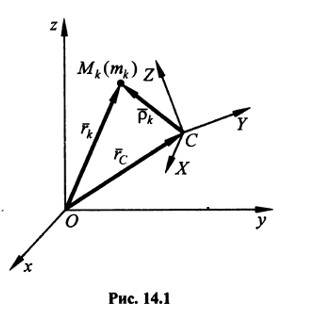
\includegraphics[scale = 0.7]{img/14.1.jpg}
    \end{figure}

\par Статический момент массы механической  системы  относительно  какой-либо точки О равен произведению массы системы $M = \sum\limits_{k=1}^N m_k$ на радиус вектор центра масс $\vec r_{c}$ :

\par $\vec S_o = \sum\limits_{k=1}^N m_k \vec r_k = M \vec r_c$,

\par откуда

\par $\vec r_c = \frac{\sum\limits_{k=1}^N m_k \vec r_k}{M}$.

\par Центр масс - это материальная точка, как бы обладающая массой системы.

\par\textbf{Теорема:}

\par Центр масс механической системы движется как материальная точка, как бы обладающая массой системы, под действием системы всех внешних сил, действующих на точки системы.

\par $\frac{Md^2 r_e}{d t^2} = \vec F^e$

\par\textbf{15.3. Теорема о движении центра масс механической системы}

\par Запишем уравнения движения механической системы в виде

\par $m_k \vec a_k = \vec F_k^e + \vec F_k^i \quad (k=1,2,...,N), \qquad(15.14)$

\par где $\vec a_k$ - ускорение k-й точки, $\vec F_k^e, \vec F_k^i$ равнодействующие внешних и внутренних сил, действующих на k-ю точку.Просуммируем уравнения (15.14) по всем точкам механической системы:

\par $\sum\limits_{k=1}^N m_k \vec a_k = \sum\limits_{k=1}^N \vec F_k^e + \sum\limits_{k=1}^N \vec F_k^i $.

\par Здесь главный вектор внутренних сил $\vec R^i = \sum\limits_{k=1}^N \vec F_k^i = 0$.

\par Продифференцировав дважды по времени выражение (14.1) для определения радиуса-вектора центра масс системы, получим

\par $M \vec\nu_c = \sum\limits_{k=1}^N m_k \vec\nu_k; \qquad (15.16)$
\par $M \vec a_c = \sum\limits_{k=1}^N m_k \vec a_k, \qquad (15.17)$

\par где $\vec\nu_c$ - абсолютная скорость центра масс системы.С учетом (15.17) уравнение (15.15) примет вид

\par $M \vec a_c = \sum\limits_{k=1}^N \vec F_k^e = \vec R^e, \qquad(15.18)$

\par где $ \vec R^e = \sum\limits_{k=1}^N \vec F_k^e$ - главный вектор внешних сил, действующих на механическую систему.

\par Теорема о движении центра масс механической системы формулируется так: центр масс механической системы движется как материальная точка, как бы обладающая массой системы, под действием системы всех внешних сил, действующих на точки системы. В проекциях на оси прямоугольной декартовой системы координат уравнения (15.18) имеют вид

\par $M \ddot x_c = \sum\limits_{k=1}^N F_kx^e; \quad M \ddot y_c = \sum\limits_{k=1}^N F_{ky}^e; \quad M \ddot z_c = \sum\limits_{k=1}^N F_{kz}^e, \qquad (15.19)$

\par где $\ddot x_c,\ddot y_c,\ddot z_c$ - проекции ускорения $\vec a_c$ центра масс механической системы.

\par Из теоремы о движении центра масс вытекают два следствия.

\par 1. Если главный вектор внешних сил, действующих на систему, равен нулю, т. е. $\vec R^e = 0$, то  из (15.18) следует, что $\vec a_c = \frac{d\vec\nu_c}{dt} = 0$, откуда после интегрирования получаем

\par $\vec\nu_c = \frac{d\vec r_c}{dt} = C_1. \qquad (15.20)$
\par Интегрируя (15.20) находим $\vec r_c = \vec C_1 t + \vec C_2. \qquad (15.21)$
Постоянные $\vec C_1, \vec C_2$ определяем из начальных условий: при t=0 $\vec r_c = \vec r_{co}, \vec\nu_c = \vec\nu_{c0}$/. Для текущего момента времени при $\vec R^e = 0$ окончательно имеем

\par $\vec\nu_c = \vec\nu_{co}; \quad \vec r_c = \vec r_{co} + \vec\nu_{co} t$.

\par Таким образом, если главный вектор внешних сил, действующих на точки механической системы, равен нулю, то центр масс механической системы движется прямолинейно и равномерно.

\par Если $\vec\nu_co = 0$, т.е. центр масс в начальный момент времени находится в покое, то

\par $\vec\nu_c = 0, \quad \vec r_c = \vec r_co, \qquad (15.22)$

\par т. е. центр масс покоится в течение всего времени движения системы при условии, что $\vec R^e = 0$.

\par 2. Пусть теперь проекция главного вектора внешних сил, действующих на систему, на одну из осей (например, ось Ox) равна нулю $R_x^e = \sum\limits_{k=1}^N F_{kx}^{(e)} = 0$, тогда из первого уравнения (15.19) следует $a_{cx} = \ddot x_c = 0$, а значит $\nu_{cx} = \dot x_c = C_1, \quad x_c = C_1 t + C_2$.

\par Постоянные определяем из начальных условий: при t=0 $x_c = x_co, \quad \nu_cx = \dot x_c = \dot x_co$. Для любого момента времени при $R_x^e = 0$ окончательно имеем

\par $\dot x_c = \dot x_co, \quad x_c = \dot x_co t + x_co$.

\par Если $\dot x_co =0$, т.е. проекция скорости центра масс на ось Ox в начальный момент времени равна нулю, то

\par $\dot x_c = 0, \quad x_c = x_{co} \qquad (15.23)$

\par в любой момент времени.
\end{center}
%7
\section{Теорема об изменении количества движения механической системы в дифференциальной и интегральной формах. Частные случаи.}
\begin{center}
    \par Запишем теорему о движении центра масс механической системы в виде:
    
    \par $M \frac{d\vec{\nu_c}}{dt} = \vec{R}^{(e)}$
    
    \par откуда получим 
    
    \par $\frac{d(M\vec{\nu_c})}{dt} = \frac{d\vec{Q}}{dt} = \vec{R}^{(e)}$
    
    \par Окончательно имеем:
    
    \par $\frac{d\vec{Q}}{dt} = \sum_{k=1}^{N} \vec{F}_{k}^{(e)} = \vec{R}^{(e)} $ \qquad (15.29)

    \par Уравнение (15.29) выражает теорему об изменении количества движения механической системы: первая производная по времени от вектора количества движения механической системы равна главному вектору внешних сил, действующих на материальные точки этой системы.

    \par В проекциях на оси прямоугольной декартовой системы координат уравнение (15.29) имеет вид:

    \par $\frac{dQ_x}{dt} = \sum_{k=1}^{N} {F}_{kx}^{(e)}; \quad \frac{dQ_y}{dt} = \sum_{k=1}^{N} {F}_{ky}^{(e)}; \quad
    \frac{dQ_z}{dt} = \sum_{k=1}^{N} {F}_{kz}^{(e)} \qquad $ (15.30) 

    \par т.е. первые производные по времени от проекций количества движения механической системы на оси координат равны сумме проекций внешних сил, действующих на точки системы, на эти же оси координат.

    \par Из  уравнения  (15.29)  получим  еще  одну  дифференциальную  форму теоремы:

    \par $d\vec{Q} = \sum_{k=1}^{N} \vec{F}_{k}^{(e)}dt = \sum_{k=1}^{N} d\vec{S}(\vec{F}_{k}^{(e)}) \qquad$ (15.31)

    \par Таким образом, дифференциал количества движения механической си-стемы равен сумме элементарных импульсов внешних сил, действующих на материальные точки системы.В проекциях на оси координат имеем:

    \par $d{Q}_x = \sum_{k=1}^{N} {F}_{kx}^{(e)}dt, \quad
    d{Q}_y = \sum_{k=1}^{N} {F}_{ky}^{(e)}dt, \quad
    d{Q}_z = \sum_{k=1}^{N} {F}_{kz}^{(e)}dt.$

    \par Проинтегрируем (15.31) по времени в пределах от 0 до t и поменяем места-ми операции интегрирования и суммирования:

    \par  $(\int_{\vec{Q}_0}^{\vec{Q}} d\vec{Q} ) = \int_{0}^{t} \sum_{k=1}^{N} \vec{F}_{k}^{(e)}dt = 
    \sum_{k=1}^{N} \int_{0}^{t} \vec{F}_{k}^{(e)}dt =
    \sum_{k=1}^{N} \vec{S}_k^{(e),}$

    \par $\vec{Q} - \vec{Q}_0 = \sum_{k=1}^{N} \vec{S}_k^{(e)} \qquad$ (15.32)

    \par Здесь $\vec{Q}=\sum_{k=1}^{N} m_k \vec{\nu}_k, \quad
    \vec{Q}_0=\sum_{k=1}^{N} m_k \vec{\nu}_{k0}$ - соответственно количества движения механической системы в произвольный и начальный моменты времени; $\vec{S}_k^{(e)}$ - полный импульс внешней силы, действующей на k-ю материальную точку.

    \par Выражение (15.32) представляет собой математическую запись теоремы об изменении количества движения механической системы в интегральной форме:  изменение  количества  движения  системы  за  время  t  равно  векторной сумме полных импульсов внешних сил, действующих на точки механической системы за то же время.

    \par В проекциях на оси координат имеем:

    \par ${Q}_x - {Q}_{x0} = \sum_{k=1}^{N} {S}_{kx}^{(e)}; \quad
    {Q}_y - {Q}_{y0} = \sum_{k=1}^{N} {S}_{ky}^{(e)}; \quad
    {Q}_z - {Q}_{z0} = \sum_{k=1}^{N} {S}_{kz}^{(e)}$

    \par Законы сохранения количества движения следуют из теоремы об изменении количества движения механической системы как частные случаи описания ее движения.

    \par \textbf{1.} Пусть главный вектор всех внешних сил, приложенных к точкам системы, равен нулю: $\vec{R}^{(e)}=\sum_{k=1}^{N} \vec{F}_k^{(e)} = 0$ Тогда из уравнения (15.29) следует, что:

    \par $\vec{Q} = \vec{C} \qquad$ (15.33)

    \par Этот  результат  (закон  сохранения  $\vec{Q}$)   формулируется  так:  если  главный вектор внешних сил, приложенных к точкам механической системы, равен нулю, то вектор количества движения системы постоянен при движении системы.

    \par В  проекциях  на  оси  прямоугольной  декартовой  системы  координат получаем:

    \par $Q_x = C_1; \quad Q_y = C_2; \quad Q_z = C_3 \qquad$ (15.34)

    \par В (15.34) входят производные от координат точек не выше первого порядка (проекции скоростей точек), т. е. эти выражения являются первыми интегралами системы дифференциальных уравнений (15.30).

    \par \textbf{2.} Пусть проекция главного вектора внешних сил на какую-либо ось координат равна нулю: $R_x^{(e)}=\sum_{k=1}^{N} F_{kx}^{(e)}=0$. Тогда из первого уравнения (15.30) следует, что:

    \par $Q_x = const$

    \par Формулируется это  так:  если  проекция  главного  вектора внешних сил, действующих на точки механической системы, на какую-либо ось равна нулю, то проекция вектора количества движения системы на ту же ось постоянна при движении системы.
    
\end{center}

%8
\section{Дифференциальные уравнения поступательного движения твердого тела.}
\begin{center}
    \par \par $M \vec a_c = \sum\limits_{k=1}^N \vec F_k^e = \vec R^e, \qquad(15.18)$

    \par где $ \vec R^e = \sum\limits_{k=1}^N \vec F_k^e$ - главный вектор внешних сил, действующих на механическую систему.
    
    \par При поступательном движении тела его угловая скорость, а следовательно, и главный момент количеств  движения относительно центра масс тождественно равны нулю. На основании теоремы о движении центра масс механической системы, уравнение (15.18) применительно к рассматриваемому случаю имеет вид:

    \par $m \vec a = \sum\limits_{k=1}^N \vec F_k^{(e)} \qquad$ (16.1)

    \par где $m$ — масса тела;  $\vec{a}$  — ускорение центра масс тела, равное ускорению любой его точки при поступательном движении.

    \par Уравнение (16.1) можно также записать в виде векторного дифференциального уравнения поступательного движения твердого тела:

    \par $m \ddot{\vec r} = \sum\limits_{k=1}^N \vec F_k^{(e)} \qquad$ (16.2)

    \par В общем случае поступательного движения тело имеет три степени свободы и его движение можно задать, определив движение центра масс тела в декартовой системе координат. В проекциях на оси декартовой системы ко-ординат для (16.2) получаем:

    \par $m \ddot{x} = \sum\limits_{k=1}^N F_{kx}^{(e)}; \qquad 
    m \ddot{y} = \sum\limits_{k=1}^N F_{ky}^{(e)}; \qquad 
    m \ddot{z} = \sum\limits_{k=1}^N F_{kz}^{(e)}$

    \par Начальные условия в данном случае имеют вид:

    \par при $t = t_0 \quad x = x_0 \quad y = y_0 \quad z = z_0 \quad \dot{x} = x_0 \quad \dot{y} = y_0 \quad \dot{z} = z_0.$

    \par В проекциях на оси естественной системы координат (при естественном способе задания движения центра масс в данном случае тело имеет одну степень свободы) уравнения (16.2) записывают так:

    \par $m \ddot{s} = \sum\limits_{k=1}^N F_{k\tau}^{(e)}; \quad
    m \frac{\dot{s}^{2}}{\rho} = \sum\limits_{k=1}^N  F_{kn}^{(e)}; \quad 
    0 = \sum\limits_{k=1}^N F_{kb}^{(e)};$

    \par где  $s=s(t)$ — закон движения центра масс тела по траектории. Начальные условия в этом случае принимают следующий вид: при $t=t_0 \quad s=s_0 \quad \dot{s} = \dot{s}_{0}.$

    \par Аналогичным  образом  можно  записать  дифференциальные  уравнения движения твердого тела в проекциях на оси любой другой инерциальной си-стемы координат и сформулировать начальные условия. Видно, что эти уравнения  подобны  дифференциальным  уравнениям  движения  материальной точки в соответствующей системе координат.
    
\end{center}
%9
\section{Кинетический момент точки и системы материальных точек относительно центра и оси.}
\begin{center}
    \par \textbf{Момент количества движения материальной точки} 
    
    \par Для характеристики движения материальной точки используют еще одну векторную меру движения — \textbf{момент количества движения}, или \textbf{кинетический момент относительно центра (точки)}.

    \par Моментом количества  движения материальной точки  массой m относительно центра O называют векторную величину, равную векторному произведению радиус-вектора материальной точки, проведенного из этого центра, на количество движения точки:
    
    \par $\vec{k}_0=\vec{M}_0(q)=\vec{r}_0 \times \vec{q} = 
    \vec{r} \times m\vec{\nu}\qquad$ (15.36)

    \par Вектор момента количества движения материальной точки строят в точке O по правилу векторного произведения (рис. 15.10).

    %рисунок 15.10
    \par \begin{figure}[H]
    \centering 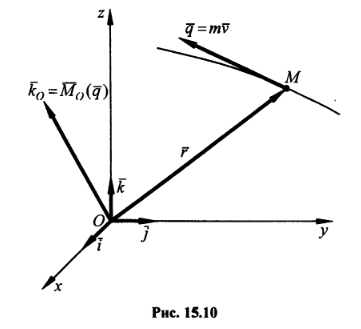
\includegraphics[scale = 0.5]{img/15.10.jpeg}
    \end{figure}

    \par Проекции вектора момента количества движения материальной точки относительно центра O на оси координат равны моментам количества движения относительно соответствующих осей координат, т.е. $(\vec{k}_0)_x=k_x, \vec{k}_0)_y=k_y, \vec{k}_0)_z=k_z$

    \par Так как

    \par $\vec{k}_0=\vec{M}_0(\vec{q})=\vec{r}\times m\vec{\nu} = m$
    \begin{vmatrix}
        \vec{i}& \vec{j}& \vec{k}\\
        x&        y&       z\\
        \nu_x&    \nu_y&    \nu_z
    \end{vmatrix},
    
    \par то моменты количества движения материальной точки относительно осей координат имеют вид:

    \par $k_x=M_x(m\vec{\nu})=m(y\nu_z-z\nu_y)=m(y\dot{z}-z\dot{y});$\qquad .......
    \par $k_y=M_y(m\vec{\nu})=m(z\nu_x-x\nu_z)=m(z\dot{x}-x\dot{z});$\quad(15.37)
    \par $k_z=M_z(m\vec{\nu})=m(x\nu_y-y\nu_x)=m(x\dot{y}-y\dot{x})$\qquad .......

    \par Единица измерения момента количества движения в СИ — килограмм-метр в квадрате на секунду  (кг · $\text {м}^{2}/c$)

    \pat \textbf{Главный момент количеств движения механической системы}

    \par Главным моментом количеств движения, или кинетическим моментом механической системы, относительно центра O называют геометрическую сумму векторов моментов количеств движения материальных точек системы относительно того же центра O:

    \par $\vec{K}_0=\sum\limits_{k=1}^N \vec{k}_{0k}=\sum\limits_{k=1}^N \vec{M}_0(\vec{q}_k)=
    \sum\limits_{k=1}^N \vec{r}_k\times m_k\vec{\nu}_k. \qquad$ (15.38)

    \par Вектор главного момента количеств движения  $\vec{K}_0$ механической системы относительно \\\ центра O строят в точке O (рис. 15.11).

    \par Проекции главного момента количеств движения  $\vec{K}_0$ системы на оси ко-ординат равны главным моментам количеств движения системы относительно соответствующих осей координат: $(\vec{K}_0)_x=K_x,\quad (\vec{K}_0)_y=K_y,\quad (\vec{K}_0)_z=K_z$

    \par С учетом (15.38) запишем главные моменты количеств движения механической системы относительно осей координат:

    \par $K_x=\sum\limits_{k=1}^N M_x(m_k \vec{\nu}_k) = 
    \sum\limits_{k=1}^N m_k(y_k \dot{z}_k - z_k \dot{y}_k);$ \qquad\qquad\quad .
    \par $K_y=\sum\limits_{k=1}^N M_y(m_k \vec{\nu}_k) = 
    \sum\limits_{k=1}^N m_k(z_k \dot{x}_k - x_k \dot{z}_k);$
    \qquad (15.39)
    \par $K_z=\sum\limits_{k=1}^N M_z(m_k \vec{\nu}_k) = 
    \sum\limits_{k=1}^N m_k(x_k \dot{y}_k - y_k \dot{x}_k).$
    \qquad\qquad\quad .

    %рисунок 15.11
    \par \begin{figure}[H]
    \centering 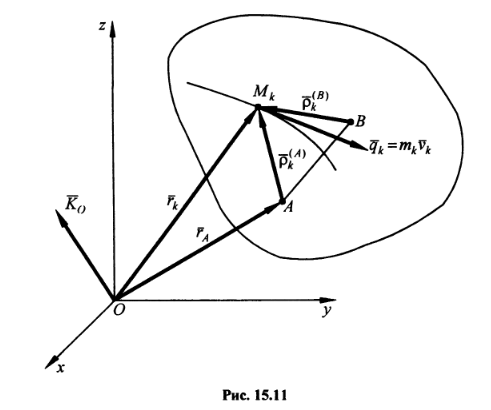
\includegraphics[scale = 0.5]{img/15.11.jpeg}
    \end{figure}

    \par \textbf{Главный момент количеств движения относительно оси  вращения при вращательном движении твердого тела}

    \par Пусть твердое тело вращается вокруг неподвижной оси Oz с угловой скоростью $\vec{\omega}$ (рис. 15.12). Определим главный момент количеств движения этого тела относительно оси Oz. Согласно определению:

    \par $K_z=\sum\limits_{k=1}^N M_z(m_k \vec{\nu}_k) \qquad$ (15.43)

    \par Проекция  скорости  точки $A_k$  тела  на касательную к траектории ее движения:

    \par $\nu_{k}__{\tau}=\omega_z h_k,$

    \par а момент количества движения относительно оси Oz:

    \par $M_z(m_k \vec{\nu}_k)=m_k\nu_{k}__{\tau}$ $h_{k}=\omega_z m_k h_k^{2},$

    \par где $\omega_z \neq 0 \quad (\omega_x = \omega_y = 0).$ Подставим $M_z(m_k \vec{\nu}_k)$ в выражение (15.43) и получим:

    \par $K_z=\omega_z \sum\limits_{k=1}^N m_k h_k^{2} = \omega_z J_z$, 

    \par где $J_z=\sum\limits_{k=1}^N m_k h_k^{2}$ - момент инерции тела относительно оси вращения Оz. Окончательно имеем:

    \par $K_z=J_z\omega_z \qquad$ (15.44)

    \par Знак $K_z$— главного момента количеств движения твердого тела относительно оси вращения — определяется знаком проекции угловой скорости $\omega_z$.

    %рисунок 15.12
    \par \begin{figure}[H]
    \centering 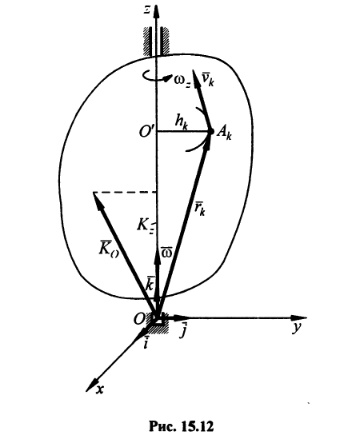
\includegraphics[scale = 0.55]{img/15.12.jpeg}
    \end{figure}

    \par Таким образом, главный момент количеств движения вращающегося тела относительно неподвижной оси вращения равен произведению момента инерции тела относительно оси вращения на проекцию угловой скорости вращения тела на ось вращения.
\end{center}
%10
\section{Теорема об изменении кинетического момента для точки и системы материальных точек. Законы сохранения кинетического момента.}
\begin{center}
    \par \textit {\underline{Теорема об изменении момента количества движения   материальной точки}}
    
    \par Запишем уравнение движения материальной точки:
    
    \par $m\frac{d\vec{\nu}}{dt}=\vec{F}$
    
    \par и умножим его векторно слева на радиус-вектор $\vec{r}\quad $(15.15)
    
    %рисунок 15.15
    \par \begin{figure}[H]
    \centering 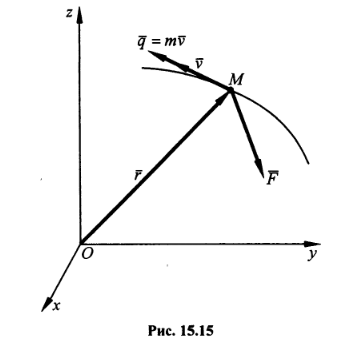
\includegraphics[scale = 0.5]{img/15.15.jpeg}
    \end{figure}
    
    \par $\vec{r}\times m\frac{d\vec{\nu}}{dt}=\vec{r}\times \vec{F}$
    
    \par Преобразуем левую часть полученного уравнения:
    
    \par $\vec{r}\times m\frac{d\vec{\nu}}{dt}=\frac{d}{dt}(\vec{r}\times m\vec{\nu})-\frac{d\vec{r}}{dt}\times m\vec{\nu}$
    
    \par Векторное произведение коллинеарных векторов $\frac{d\vec{r}}{dt}\times m\vec{\nu}=\vec{\nu}\times m\vec{\nu}=0$, поэтому получаем:
    
    \par $\frac{d(\vec{r}\times m\vec{\nu})}{dt}=\frac{d\vec{k}_0}{dt}=\vec{r}\times \vec{F}=\vec{M}_0(\vec{F})$
    
    \par или 
    
    \par $\frac{d\vec{k}_0}{dt}=\vec{M}_0(\vec{F})\quad$(15.54)
    
    \par Уравнение  (15.54)  выражает  теорему об  изменении  момента  количества  движения материальной точки: первая производная по времени от момента количества движения  точки  относительно  центра  O равна  моменту  равнодействующей  силы относительно того же центра O.
    
    \par В проекциях на оси прямоугольной декартовой системы координат имеем:
    
    \par $\frac{d{k}_x}{dt}={M}_x(\vec{F})\quad$
    $\frac{d{k}_y}{dt}={M}_y(\vec{F})\quad$
    $\frac{d{k}_z}{dt}={M}_z(\vec{F})\quad\qquad$ (15.55)

    \par \textit {\underline{Теорема об изменении главного момента количеств  движения механической системы}}
    
    \par Рассмотрим механическую систему $M_k$ (k=1,2,...,N), состоящую из N материальных  точек,  к  каждой  из  которых  приложены  равнодействующие внешних $\vec{F}_k^{(e)}$ и внутренних $\vec{F}_k^{(i)}$ сил. Для каждой точки $M_k$ запишем теорему об  изменении  момента  количества  движения  относительно  неподвижного центра O (рис. 15.16):
    
    \par $\frac{d}{dt}(\vec{r}_{k}\times m_k\vec{\nu}_k)=\vec{r}_{k}\times \vec{F}_k^{(e)}+\vec{r}_{k}\times \vec{F}_k^{(i)}\qquad$ (15.56)

    \par Просуммировав (15.56) по всем точкам:

    \par $\sum\limits_{k=1}^N\frac{d}{dt}(\vec{r}_{k}\times m_k\vec{\nu}_k)=\sum\limits_{k=1}^N\vec{r}_{k}\times \vec{F}_k^{(e)}+\sum\limits_{k=1}^N\vec{r}_{k}\times \vec{F}_k^{(i)}\qquad$

    \par и преобразовав левую часть уравнения, получим:

    \par $\sum\limits_{k=1}^N\frac{d}{dt}(\vec{r}_{k}\times m_k\vec{\nu}_k) = \frac{d}{dt}\sum\limits_{k=1}^N(\vec{r}_{k}\times m_k\vec{\nu}_k)=\frac{d\vec{K}_0}{dt}$
    
    %рисунок 15.16
    \par \begin{figure}[H]
    \centering 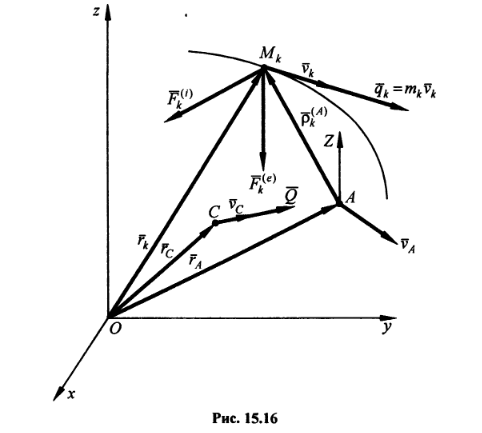
\includegraphics[scale = 0.5]{img/15.16.jpeg}
    \end{figure}
    
    \par $\sum\limits_{k=1}^N \vec{r}_{k}\times m_k \vec{\nu}_k$ - главный момент количеств движения  механической системы относительно центра O.

    \par Главный момент внутренних сил:

    \par $\vec{L}_0^{(i)}=\sum\limits_{k=1}^N \vec{r}_{k}\times \vec{F}_k^{(i)}=0 \qquad$ (15.57)

    \par а главный момент внешних сил:

    \par $\vec{L}_0^{(e)}=\sum\limits_{k=1}^N \vec{r}_{k}\times \vec{F}_k^{(e)}=\sum\limits_{k=1}^N \vec{M}_0(\vec{F}_k^{(e)}) \qquad$ (15.58)

    \par Окончательно имеем:

    \par $\frac{d\vec{K}_0}{dt}=\sum\limits_{k=1}^N \vec{M}_0(\vec{F}_k^{(e)})=\vec{L}_0^{(e)}\qquad$ (15.59)

    \par Уравнение (15.59) выражает теорему об изменении главного момента количеств движения механической системы: первая производная по времени от главного момента количеств движения механической системы относительно неподвижного центра O равна главному моменту внешних сил, приложенных к точкам системы, относительно того же центра.

    \par В проекциях на оси прямоугольной декартовой системы координат получаем соотношения, выражающие  теоремы  об изменении  главного  момента количеств движения системы относительно осей координат:

    \par $\frac{d{K}_x}{dt}=\sum\limits_{k=1}^N {M}_x(\vec{F}_k^{(e)})={L}_x^{(e)};\qquad \frac{d{K}_y}{dt}=\sum\limits_{k=1}^N {M}_y(\vec{F}_k^{(e)})={L}_y^{(e)}; \qquad \frac{d{K}_z}{dt}=\sum\limits_{k=1}^N {M}_z(\vec{F}_k^{(e)})={L}_z^{(e)} \qquad$ (15.60)

    \par \textit {\underline{Законы сохранения главных моментов   количеств движения системы}}    

    \par Законы сохранения моментов количества движения и главных моментов количеств движения при движении материальной точки и механической системы записываются одинаково, так как материальная точка есть механическая система, состоящая из одной точки. Рассмотрим частные случаи теоремы об изменении главного момента количеств движения механической системы.

    \par {1.} Пусть главный момент внешних сил системы относительно центра O равен нулю, т.е. $\vec{L}_{0}^{(e)}=0$. Тогда, согласно (15.59),

    \par $\frac{d\vec{K}_{0}}{dt}=0 \qquad$(15.65)

    \par Интегрируя (15.65), получаем:

    \par $\vec{K}_{0}=\overrightarrow{const},$

    \par т.е. главный момент количеств движения механической системы относительно центра O постоянен по модулю и направлению. Это уравнение выражает закон сохранения главного момента количеств движения механической системы относительно центра O в векторной форме: если главный момент внешних сил относительно неподвижного центра O равен нулю, то главный момент количеств движения механической системы относительно этого центра постоянен по модулю и направлению.

    \par В проекциях на оси прямоугольной декартовой системы координат получаем уравнения:

    \par $K_x=C_1; \quad K_y=C_2; \quad K_z=C_3,$

    \par которые выражают законы сохранения главных моментов количеств движения системы относительно осей координат (частные случаи теоремы об изменении главного момента количеств движения системы относительно осей координат)  и  представляют  собой  первые  интегралы  дифференциальных уравнений для механической системы.

    \par {2.} Пусть сумма моментов внешних сил, действующих  на механическую систему, относительно оси Ox равна нулю, т.е. ${L}_{x}^{(e)}=0.$ Тогда, согласно (15.60),

    \par $\frac{d{K}_{x}}{dt}=0; \quad K_{x}=const$

    \par Следовательно, если главный момент внешних сил, действующих на механическую систему, относительно какой-либо оси равен нулю, то главный момент количеств движения механической системы относительно этой оси постоянен.

    \par Если рассматривается тело или система тел, вращающихся вокруг непод-вижной оси Oz с угловой скоростью $\omega_z$ и ${L}_{z}^{(e)}=0,$ то $K_z=J_z\omega_z=const.$ Если в начальном состоянии угловая скорость и момент инерции системы относительно оси Oz будут соответственно $\omega_{0z}$ и $J_{0z},$ то

    \par $J_{0z}\omega_{0z}=const\quad$ и $\quad J_{z}\omega_{z}=J_{0z}\omega_{0z}$

    \par \textit{Можно рассказать про скамью Жуковского, но это уж явно на ваше усмотрение и желательно устно:)}
\end{center}
%11
\section{Кинетический момент твердого тела относительно оси вращения.}
\begin{center}
    \par \textbf{Главный момент количеств движения относительно оси  вращения при вращательном движении твердого тела}

    \par Пусть твердое тело вращается вокруг неподвижной оси Oz с угловой скоростью $\vec{\omega}$ (рис. 15.12). Определим главный момент количеств движения этого тела относительно оси Oz. Согласно определению:

    \par $K_z=\sum\limits_{k=1}^N M_z(m_k \vec{\nu}_k) \qquad$ (15.43)

    \par Проекция  скорости  точки $A_k$  тела  на касательную к траектории ее движения:

    \par $\nu_{k}__{\tau}$=${\omega}_{z} h_k,$

    \par а момент количества движения относительно оси Oz:

    \par $M_z(m_k \vec{\nu}_k)=m_k\nu_{k}__{\tau}$ $h_{k}=\omega_z m_k h_k^{2},$

    \par где $\omega_z \neq 0 \quad (\omega_x = \omega_y = 0).$ Подставим $M_z(m_k \vec{\nu}_k)$ в выражение (15.43) и получим:

    \par $K_z=\omega_z \sum\limits_{k=1}^N m_k h_k^{2} = \omega_z J_z$, 

    \par где $J_z=\sum\limits_{k=1}^N m_k h_k^{2}$ - момент инерции тела относительно оси вращения Оz. Окончательно имеем:

    \par $K_z=J_z\omega_z \qquad$ (15.44)

    \par Знак $K_z$— главного момента количеств движения твердого тела относительно оси вращения — определяется знаком проекции угловой скорости $\omega_z$.

    %рисунок 15.12
    \par \begin{figure}[H]
    \centering 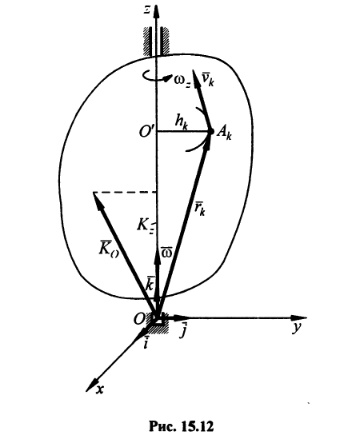
\includegraphics[scale = 0.5]{img/15.12.jpeg}
    \end{figure}

    \par Таким образом, главный момент количеств движения вращающегося тела относительно неподвижной оси вращения равен произведению момента инерции тела относительно оси вращения на проекцию угловой скорости вращения тела на ось вращения.
\end{center}
%12
\section{Дифференциальное уравнение вращения тела вокруг неподвижной оси.}
\begin{center}
  \par{(15.60) \quad ${\frac{dK_x}{dt}} ={\sum\limits_{k=1}^N M_x (\vec{F}_k^{(e)})} = \vec{L}_x^{(e)}; \quad 
  {\frac{dK_y}{dt}} ={\sum\limits_{k=1}^N M_y (\vec{F}_k^{(e)})}= \vec{L}_y^{(e)}; \quad
  {\frac{dK_z}{dt}} ={\sum\limits_{k=1}^N M_z (\vec{F}_k^{(e)})}= \vec{L}_z^{(e)}; \quad$}
  \hfill \break
  \par В случае вращения вокруг неподвижной оси тело имеет одну степень свободы. Для получения дифференциального уравнения вращательного движения твердого тела воспользуемся теоремой об изменении главного момента количеств движения механической системы относительно оси вращения Oz, записав (15.60) в виде:
  \par $ \frac{dK_z}{dt} = \sum_{k=1}^N {M_z} {(\vec{F}_k^{(e)})} $
  \par где для твердого тела $ {K_z} = {J_z} {\omega_z} = {J_z \dot{\varphi} }$. Тогда 
  \par ${J_z}{\ddot{\varphi}} = \sum_{k=1}^N {M_z} {(\vec{F}_k^{(e)})} \qquad$ (16.3)
  \par Выражение (16.3) называется дифференциальным уравнением вращения твердого тела вокруг неподвижной оси. Его можно также записать в виде
  \par ${J_z} \frac{d \omega_z}{dt} = \sum_{k=1}^N {M_z} {(\vec{F}_k^{(e)})}$ или ${J_z}{\varepsilon_z} = \sum_{k=1}^N {M_z} {(\vec{F}_k^{(e)})} $
  \par Начальные условия для случая вращения твердого тела вокруг неподвижной оси следующие: ${t=t_0}$ ${\varphi = \varphi_0}$, ${\dot{\varphi} = {\omega_z} = {\dot{\varphi}_0}}$ 
\end{center}
%13
\section{Моменты инерции системы и твердого тела. относительно оси и полюса. Формула для вычисления момента инерции относительно оси любого направления.}
\begin{center}
    \par При рассмотрении вращательных движений твердых тел вводят понятия моментов инерции, которые характеризуют распределение массы тела по отношению к точке (полюсу) оси или плоскости.
    \par Моментом инерции материальной точки М относительно точки О называется произведение массы m этой точки на квадрат расстояния r до точки O: 
    \par ${j_0=mr^2}$
    \par Рассмотрим механическую систему,состоящую из N материальных точек с массами ${m_k} {(k=1,2,...,N)}$.Момент инерции механической системы, состоящей из N материальных точек $M_k$, относительно точки (полюса) О равен сумме моментов инерции этих точек (рис.14.2) (Будет внизу)
    \par ${J_0} = {{\sum_{k=1}^N {j_0^{(k)}}} ={\sum_{k=1}^N {m_k r_k^2}}} $
    \par Момент инерции относительно точки называют полярным моментом инерции.
    \par Моментом инерции механической системы материальных точек относительно оси Ol называется сумма произведений масс этих точек на квадраты их расстояний до оси Ol (см.рис.14.2):
    \par ${J_i}= {{\sum_{k=1}^N {m_k h_k^2}}} $
    \par Для тела, имеющего непрерывное распределение массы, имеем соответственно интегралы по массе М:
    \par $ J_0 = \int_{(M)} r^2dm$ ; $ J_i = \int_{(M)} h^2dm$
    \par Величина 
    \par $\rho_i = \sqrt{\frac{J_i}{M}} \qquad$ (14.4)
    \par называется радиусом инерции тела относительно оси Ol. Тогда момент инерции можно представить как 
    \par $ J_i = M \rho_i^2$
        \begin{figure}[H]
        \centering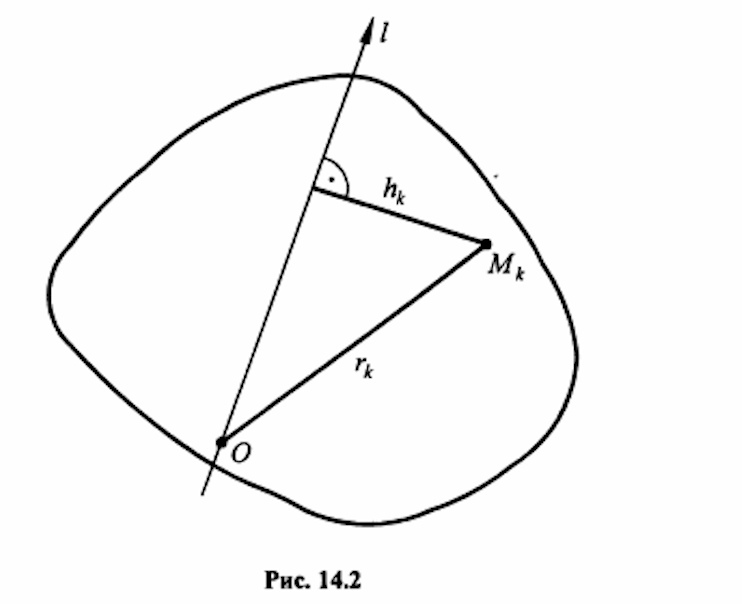
\includegraphics[scale=0.25]{img/14.2.jpeg} 
        \end{figure}
    \par Значения $\rho_i$ можно вычислить по формуле (14.4), при этом М $M$ и $J_i$ определяют экспериментально. 
    \par Единица измерения момента инерции килограмм на квадратный метр (кг $м^2$)
    \par Моменты инерции относительно декартовых осей Ox,Oy,Oz и полюса О определяют по формулам (рис.14.3)
    \par ${J_x} = {\sum_{k=1}^N {m_k (y_k^2 + z_k^2)}}$
    \par ${J_y} = {\sum_{k=1}^N {m_k (x_k^2 + z_k^2)}} \qquad$ (14.5)
    \par ${J_z} = {\sum_{k=1}^N {m_k (x_k^2 + y_k^2)}}$    
    \par ${J_{()}} = {\sum_{k=1}^N {m_k r_k^2}} = {\sum_{k=1}^N {m_k (x_k^2 + y_k^2 + z_k^2)}} \qquad$  (14.6)
    
    \begin{figure}[H]
        \centering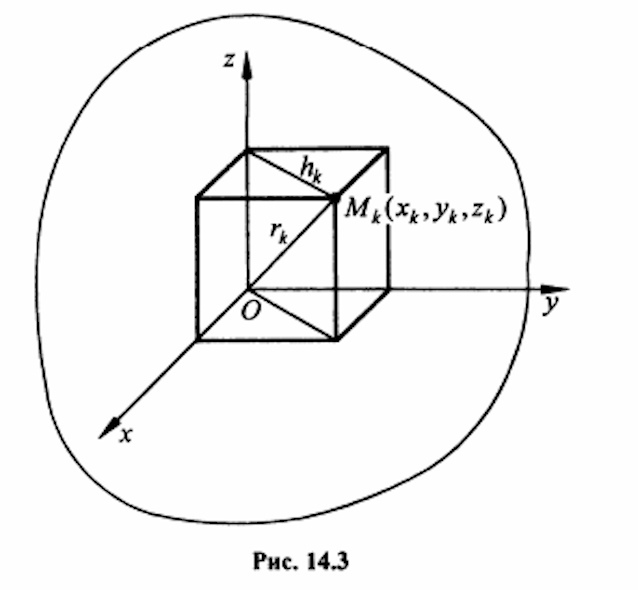
\includegraphics[scale=0.3]{img/14.3.jpeg} 
    \end{figure}
    \par Сложив левые и правые части уравнений системы (14.5), получим 
    \par $ 2J_{()} = J_x + J_y + J_z \qquad$ (14.7)
    \par Моменты инерции относительно координатных плоскостей Oxy,Oyz,Oxz соответственно равны:
    \par ${J_{Oxy}} = {\sum_{k=1}^N {m_k z_k^2}}$  ${J_{Oyz}} = {\sum_{k=1}^N {m_k x_k^2}}$  ${J_{Oxz}} = {\sum_{k=1}^N {m_k y_k^2}}\qquad$ (14.8)
    \par Для тела,имеющего непрерывное распределение массы, осевые моменты инерции относительно осей координат определяются интегралами по массе М:
    \par $ J_x = \int_{M} (y^2+z^2)dm$ $ J_y =\int_{M} (x^2+z^2)dm$ $ J_z = \int_{M} (x^2+y^2)dm$
    \par
    \par Зависимость моментов инерции относительно параллельных осей (теорема Гюйгенса-Штейнера)
    \par
    \par Найдем зависимость между моментами инерции механической системы относительно параллельных осей Oz и Cz (рис 14.4)
    \begin{figure}[H]
        \centering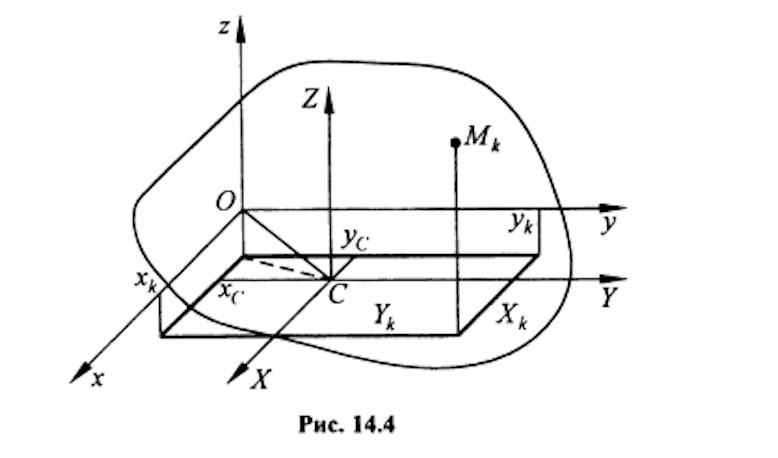
\includegraphics[scale=0.3]{img/14.4.jpeg} 
    \end{figure}
    \par Выберем две системы прямоугольных декартовых координат Oxyz и CXYZ оси параллельны, а точка С- центр масс системы. Моменты инерции относительно осей Оz и Cz будут соответсвенно равны 
    \par $ j_{Oz} = \sum_{k=1}^N {m_k (x_k^2+y_k^2)}$; $ j_{CZ} = \sum_{k=1}^N {m_k (X_k^2+Y_k^2)}$
    \par Координаты точки $M_k$ в рассматриваемых системах связаны уравнениями 
    \par $x_k= X_k+x_c$ ; $y_k= Y_k+y_c$
    \par Подставив выражение для $J_{Oz}$ эти соотношения, получим 
    $J_{Oz} = \sum_{k=1}^N  {m_k[(X_k+x_c)^2 + (Y_k + y_c)^2]} = \sum_{k=1}^N {m_k (X_k^2 + Y_k^2)} + 2x_c \sum_{k=1}^N {m_k X_k} + 2y_c \sum_{k=1}^N {m_k Y_k} + (x^2_c+y^2_c) \sum_{k=1}^N {m_k} $
    \par Здесь $\sum_{k=1}^N {m_k}= M$ - масса системы; $\sum_{k=1}^N {m_k  X_k} = MX_c=0$ $\sum_{k=1}^N {m_k Y_k} =MY_c=0 $, так как $X_c=Y_c=0; x_c^2+y^2_c=d^2$, d - расстояние между осями Oz и CZ
    \par Окончательно имеем 
    \par $J_{Oz} = J_{CZ} + Md^2$
    \par Полученное выражение представляет собой математическую запись теоремы Гюйгенса-Штейнера,  которую можно сформулировать так: момент инерции системы относительно какой-либо оси равен сумме момента инерции относительно параллельной оси, проходящей через центр масс системы, и произведения массы системы на квадрат расстояния между параллельными осями
\end{center}

%14
\section{Эллипсоид инерции. Главные оси инерции симметричных твердых тел.}
\begin{center}
    \par \textbf{Эллипсоид инерции} — поверхность второго порядка, построенная в любой точке  —  характеризует  спектр  моментов  инерции  тела  относительно  осей, проходящих через эту точку. Для построения этой поверхности на каждой оси Ol, проходящей через точку O, откладывают от этой точки отрезок

    \par $OK = \frac{1}{\sqrt{J_l}}$

    \par Геометрическое место концов отрезков OK (точек K) и является эллипсо-идом инерции.Получим  уравнение  эллипсоида  инерции  в  системе  координат  Oxyz (рис. 14.18). Подставив выражения $\cos{\alpha} = \frac{x}{OK} = \sqrt{J_l} x, \quad \cos{\beta} = \frac{y}{OK} = \sqrt{J_l} y, \quad \cos{\gamma} = \frac{z}{OK} = \sqrt{J_l} z$ в формулу (14.13), получим

    \par $J_x x^2 + J_y y^2 + J_z z^2 - 2J_xy xy - 2J_xz xz - 2J_yz yz = 1 \qquad (14.15)$

    \begin{figure}[H]
    \centering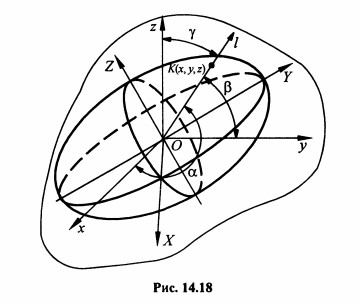
\includegraphics[scale=0.7]{img/14.18.jpg} 
    \end{figure}

    \par Для каждой точки тела существует свой эллипсоид инерции. Если оси ко-ординат  направить по  взаимно  перпендикулярным  главным  осям эллипсоида инерции (OX, OY, OZ  на рис. 14.18), то его уравнение будет иметь следующий вид:

    \par $J_X X^2 + J_Y Y^2 + J_Z Z^2 = 1 \qquad (14.16)$
    \par Главные  оси  (оси  симметрии)  эллипсоида  инерции,  построенного  в точке твердого тела, называются \textbf{главными осями инерции} для данной точки тела. Следовательно, в каждой точке тела имеются три главные оси инерции, которые являются главными осями эллипсоида инерции, построенного в данной точке.Эллипсоид  инерции,  построенный  для  центра  масс  тела,  называется \textbf{центральным эллипсоидом инерции}, а его главные оси — главными центральными  осями  инерции  тела.  Моменты  инерции  тела  относительно  главных осей инерции в точке называются \textbf{главными моментами инерции} для этой точки тела. В формуле (14.16)  это $J_X, J_Y, J_Z$. Моменты инерции относительно главных центральных осей инерции называют главными центральными моментами инерции тела и обозначают $J_CX, J_CY, J_CZ$. Сравнив уравнение (14.16) с уравнением эллипсоида инерции, записанным в канонической форме:

    \par $\frac{X^2}{a^2} + \frac{Y^2}{b^2} + \frac{Z^2}{c^2} = 1 \qquad (14.17)$
    \par получим
    \par a = $\frac{1}{\sqrt{J_X}}; \quad b = \frac{1}{\sqrt{J_Y}}; \quad c = \frac{1}{\sqrt{J_Z}}$,

    \par т. е. большей оси эллипсоида инерции соответствует меньший главный момент инерции тела для данной точки.Эллипсоид инерции называется \textbf{трехосным}, если все главные моменты инерции для  точки  тела  различны,  и  \textbf{эллипсоидом}вращения,  если  два  главных  момента  инерции  для  точки  тела  равны.  Все  прямые,  расположенные в плоскости, перпендикулярной оси вращения, являются главными осями инерции тела в точке. Эллипсоид инерции становится сферой, если все главные моменты инерции тела в точке равны. Все оси инерции, проходящие через центр сферы, являются главными.Уравнения эллипсоида инерции (14.16), (14.17) не содержат центробежных моментов инерции, т. е. центробежные моменты инерции относительно главных осей инерции равны нулю:
    \par $J_XY = J_XZ = J_YZ = 0. \qquad (14.18)$
    \par Справедливо  и  обратное  утверждение: чтобы оси прямоугольной системы  координат были главными осями инерции, необходимо и достаточно выполнить условия (14.18).Запишем формулу (14.13), когда оси OX, OY, OZ являются главными осями инерции в точке O. В этом случае все центробежные моменты инерции равны нулю и
    \par $J_l = J_X \cos^2{\alpha} + J_Y \cos^2{\beta} + J_Z \cos^2{\gamma}. \qquad (14.19)$

    \par \begin{figure}[H]
    \centering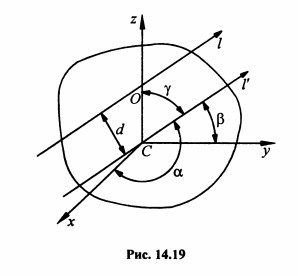
\includegraphics[scale=0.7]{img/14.19.jpg} 
    \end{figure}

    \par С помощью этой формулы при известных главных моментах инерции в точке O определяют момент инерции относительно оси Ol.Моменты инерции относительно произвольной оси Ol (рис. 14.19), согласно выражению (14.19) и теореме Гюйгенса — Штейнера, вычисляют по формуле
    \par $J_l = J_Y +M d^2 = J_CX \cos^2{\alpha} + J_CY \cos^2{\beta} + J_CZ \cos^2{\gamma} + M d^2$,
    
    \par где $J_CX, J_CY, J_CZ, M, d$  —  главные  центральные  моменты  инерции  тела,  его масса и расстояние между осью Ol и параллельной ей осью  Cl′,  проходящей через центр масс тела.

    
\end{center}
%15
\section{Кинетический момент твердого тела при сферическом движении.}
\begin{center}
    \par Твёрдое тело с закреплённой точкой  при движении в любой момент времени имеет угловую скорость $\vec\omega$. Главный момент количеств движения тела относительно неподвижной точки

     \par $\vec K_0 = \sum\limits_{k=1}^N \vec r_k \times m_k \vec\nu_k$,

     \par где $\vec\nu_k = \vec\omega \times \vec r_k$.

	  \par Тело разбито на N элементов  с массой $m_k$ и абсолютной  скоростью $\vec\nu_k$ (рис. 15.13).
	  \par Проекция $\vec K_O$ на оси $O_xyz$, а следовательно, и главные моменты количеств движения тела относительно осей координат, и проекции скорости точки $\vec\nu_k$ на оси координат определяются формулами (15.39) и (4.7). С учётом (15.39) и (4.7) для оси $O_z$ получаем

	  \par $K_x = \sum\limits_{k=1}^N m_k(y_k \nu_kz - z_k \nu_ky) = \sum\limits_{k=1}^N m_k[y_k(\omega_x y_k - \omega_y x_k) - z_k(\omega_z x_k - \omega_x z_k)] = \omega_x \sum\limits_{k=1}^N m_k(y_k^2 + z_k^2) - \omega_y \sum\limits_{k=1}^N m_k x_k y_k - \omega_z \sum\limits_{k=1}^N m_k x_k z_k$.

	  \par Проекции угловой скорости здесь являются кинематическими инвариантами и вынесены за знаки сумм, а суммы есть осевой $J_x$ и центробежные $J_xy, J_xz$ моменты инерции. Аналогично можно  получить зависимости для $K_y, K_z$.

	  \par \begin{figure}[H]
        \centering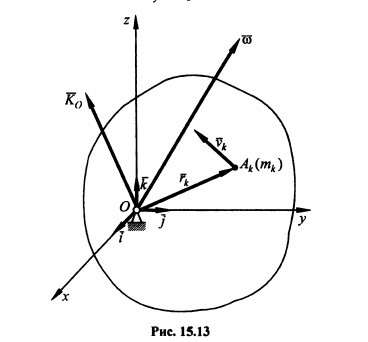
\includegraphics[scale=0.7]{img/15.13.jpg} 
        \end{figure}

	  \par Окончательно формулы для главных моментов количеств движения тела относительно осей координат с началом в неподвижной точке примут вид

	  \par $K_x = J_x \omega_x - J_xy \omega_y - J_xz \omega_z$;
	  \par $K_y = -J_yx \omega_x + J_y \omega_y - J_yz \omega_z$;
	  \par $K_z = -J_zx \omega_x - J_zy \omega_y + J_z \omega_z$. 
   \par Уравнения (15.46) имеют одинаковый вид как для неподвижных, так и для подвижных, например, жёстко связанных с телом, осей. 
	  Главный момент количеств движения твёрдого тела относительно точки O определяется по формуле

	  \par $\vec K_O = K_z \vec i + K_y \vec j + K_z \vec k$

	  \par независимо от того, какие оси координат выбраны. Использовав выражение для тензора инерции (14.14) и правило умножения тензора на вектор-столбец проекций мгновенной угловой скорости тела, получим

	  \par $\vec K_O = J \vec\omega$,

	  \par где  \begin{equation*}
						\vec K_O = \left(
						\begin{array}{c}
							K_x\\
							K_y\\ 
							K_z\\  
						\end{array}
						\right)
					\end{equation*};
					      \begin{equation*}
							   \vec\omega = \left(
								\begin{array}{c}
									\omega_x\\
									\omega_y\\ 
									\omega_z\\  
								\end{array}
								\right)
							\end{equation*}.
       \par Выражения (15.46) упрощаются, если для тела выбранные оси являются главными осями инерции в точке О (т.е. $J_XY = J_XZ = J_YZ = 0)$. Тогда

	  \par $K_X = J_X \omega_X; \quad K_Y = J_Y \omega_Y; \quad K_Z = J_Z \omega_Z$.
    
\end{center}
%16
\section{Кёнигова система отсчета. Кинетический момент системы материальных точек при сложном движении.}
\begin{center}
  \par Введём подвижную систему координат CXYZ, которая движется поступательно по отношению к инерциальной системе отсчёта $O_{xyz}$ и начало которой связано с центром масс C системы. Подвижную систему CXYZ называют кёнинговой системой координат (рис. 15.14).
	  \par Для краткости движение механической системы по отношению к CXYZ будем называть  движением системы относительно её центра масс. Запишем выражение $\vec r_k = \vec r_C + \vec\rho_k$, справедливое в любой момент времени движения механической системы, и продифференцируем его по времени:

	  \par $\frac{d \vec r_k}{dt} = \frac{d \vec r_c}{dt} + \frac{d \vec\rho_k}{dt}$.
     
	  \par Тогда

	  \par $\vec\nu_k = \vec\nu_C + \vec\nu_k^r$.

	  \par Здесь $\vec\nu_k$ - абсолютная скорость точки $M_k$, а $\vec\nu_C$ - абсолютная скорость центра масс механической системы. Докажем, что $\vec\nu_k^r$ - относительная скорость точки $M_k$ по отношению к системе координат CXYZ.

	  \par \begin{figure}[H]
     \centering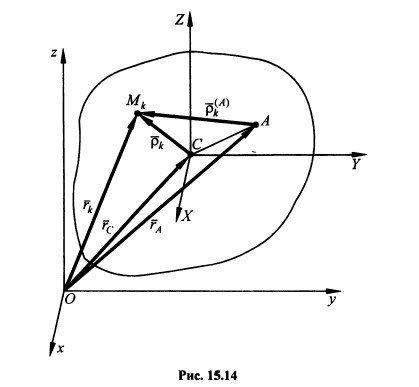
\includegraphics[scale=0.7]{img/15.14.jpg} 
     \end{figure}

	  \par Согласно формуле Бура,

	  \par $\frac{d \vec\rho_k}{dt} = \frac{\widetilde{d} \vec\rho_k}{dt} + \vec\omega \times \vec\rho_k$,

	  \par где $\frac{\widetilde{d} \vec\rho_k}{dt}$ - локальная производная в подвижной системе координат. Но при поступательном движении системы CXYZ

	  \par $\frac{\widetilde{d} \vec\rho_k}{dt} = \vec\nu_k^r = \frac{d \vec\rho_k}{dt}$.

	  \par Главный момент количеств движения механической системы относительно неподвижного центра О для абсолютного движения системы относительно неподвижной (инерциальной) системы координат $O_{xyz}$ равен (см. рис. 15.11)

	  \par $\vec K_O = \sum\limits_{k=1}^N \vec r_k \times m_k \vec\nu_k. \qquad (15.50)$

	  \par Подставляя в (15.50) выражения для $\vec r_k$ и $\vec\nu_k$, после некоторых преобразований получаем
	  
	  \par $\vec K_O = \sum\limits_{k=1}^N (\vec r_C + \vec\rho_k) \times m_k(\vec\nu_C + \vec\nu_k^r) = \vec r_C \times \vec\nu_C \sum\limits_{k=1}^N m_k + \vec r_C \times \sum\limits_{k=1}^N m_k \vec\nu_k^r + \sum\limits_{k=1}^N m_k \vec\rho_k \times \vec\nu_C + \sum\limits_{k=1}^N \vec\rho_k \times m_k \vec\nu_k^r. \qquad (15.51)$

	  \par Здесь $\sum\limits_{k=1}^N m_k \vec\rho_k = M \vec\rho_C = 0$, так как радиус вектор центра масс относительно центра масс $\vec\rho_C = 0$, а следовательно,

	  \par $\sum\limits_{k=1}^N m_k \vec\nu_k^r = \frac{d}{dt}(\sum\limits_{k=1}^N m_k \vec\rho_k) = 0$,

	  \par т.е. количество движения системы в её движении относительно центра масс равно нулю. Таким образом, уравнение (15.51) принимает вид

	  \par $\vec K_O = \vec r_C \times M \vec\nu_C + \vec K_C^r = \vec M_O(\vec Q) + \vec K_C^r, \qquad (15.52)$

	  \par где $\vec K_C^r = \sum\limits_{k=1}^N \vec\rho_k \times m_k \vec\nu_k^r$ - главный момент количеств движений механической системы относительно центра масс для относительного движения системы по отношению к уентру масс ( по отношению к системе координат CXYZ, движущейся поступательно  вместе с центром масс).
	  \par Таким образом, главный момент количеств движения механической системы относительно неподвижного центра О для обсолютного движения системы равен векторной сумме момента вектора количества абсолютного движения системы (приложенного в центре масс) относительно того же центра, и главного момента количеств движения системы относительно центра масс для относительного движения системы по отношению к центру масс. В проекции на ось $O_z$(CZ) формула (15.52) принимает вид
	  
	  \par $K_z = M_z (\vecQ) + K_{CZ}^r, \qquad (15.53)$

	  \par где $K_{CZ}^r$ - главный момент количеств движения системы относительно оси CZ, проходящей через центр масс системы праллельно оси $O_z$.

	  \par При плоскопараллельном движении твёрдого тела, если ось CZ перпендикулярна плоскости движения тела, $K_{CZ}^r = J_{CZ} \omega_Z$, где $J_{CZ}$ - момент инерции тела относительно оси CZ (относительным движением тела является его вращение вокруг оси  CZ). 
\end{center}
%17
\section{Теорема об изменении кинетического момента системы в относительном движении по отношению к центру масс.}
\begin{center}
    \par Пусть подвижная система координат CXYZ связана с цент ром масс и движется поступательно относительно неподвижной системы $O_{xyz}$ (рис. 15.17). Согласно теореме об изменении главного момента количеств движения системы относительно центра O для абсолютного движения механической системы,

	  $$\frac{d \vec K_O}{dt} = \sum\limits_{k=1}^N \vec r_k \times \vec F_k^r$$,

	  \par а также с учётом (15.52) и $\vec r_k = \vec r_C + \vec\rho_k$ запишем

	  $$\frac{d}{dt} [\vec r_C \times \vec Q + \vec K_C^r] = \frac{d \vec r_C}{dt} \times \vec Q + \vec r_C \times \frac{d \vec Q}{dt} + \frac{d \vec K_C^r}{dt} = \sum\limits_{k=1}^N (\vec r_C + \vec\rho_k) \times \vec F_k^e$$.

	  \par Но $\frac{d \vec r_C}{dt} \times \vec Q = \vec\nu_C \times M \vec\nu_C = 0$ как  векторное  произведение  коллинеарных векторов. Используя теорему об изменении количества движения механической системы $ \frac{d \vec Q}{dt} = \sum\limits_{k=1}^N \vec F_k^e$, получаем

	  $$\frac{d \vec K_C^r}{dt} = \vec r_C \times (\sum\limits_{k=1}^N \vec F_k^e - \frac{d \vec Q}{dt}) + \sum\limits_{k=1}^N \vec\rho_k \times \vec F_k^e$$.

	  \par Окончательно имеем

	  $$\frac{d \vec K_C^r}{dt} = \sum\limits_{k=1}^N \vec\rho_k \times \vec F_k^e = \vec L_C^e, \qquad (15.63)$$

	  \par где $\sum\limits_{k=1}^N \vec\rho_k \times \vec F_k^e = \vec L_C^e$ - главный момент внешних сил относительно центра масс С.

     \par \begin{figure}[H]
     \centering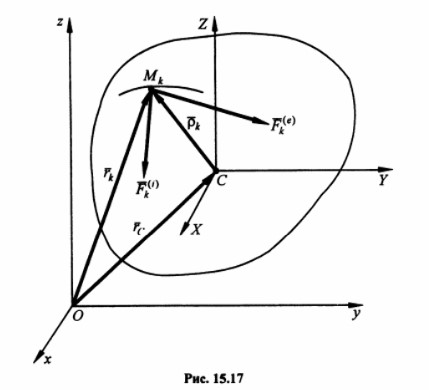
\includegraphics[scale=0.7]{img/15.17.jpg} 
     \end{figure} 

	  \par Сформулируем теорему: первая производная по времени от главного момента количеств движения системы, вычисленного относительно центра масс для относительного движения механической системы по отношению к центру масс (по отношению к системе координат, движущейся поступательно вместе с центром масс), равна главному моменту внешних сил, действующих на точки системы, относительно центра масс.

	  \par В проекциях на оси подвижной системы координат CXYZ имеем

	  $$\frac{d K_{CX}^r}{dt} = \sum\limits_{k=1}^N M_{CX} (\vec F_k^e) = L_{CX}^e;$$
	  $$\frac{d K_{CY}^r}{dt} = \sum\limits_{k=1}^N M_{CY} (\vec F_k^e) = L_{CY}^e; \qquad (15.64)$$
	  $$\frac{d K_{CZ}^r}{dt} = \sum\limits_{k=1}^N M_{CZ} (\vec F_k^e) = L_{CZ}^e$$.

   \par Уравнения  (15.64)  выражают  теорему  об  изменении  главного  момента количеств движения механической системы относительно осей, проходящих через центр масс, при относительном движении механической системы по отношению к центру масс.

\end{center}
%18
\section{Дифференциальные уравнения плоского движения твердого тела.}
\begin{center}
    \par \textbf{Плоское движение твердого тела}
        $$M \vec a_{c} = \sum_{k=1}^N \vec F_{k}^{(e)} = \vec R^{(e)} \qquad (15.18)$$
    \par \textbf{Дифференциальные уравнения плоского движения твердого тела} получим на основании теорем о движении центра масс и об изменении главного момента количеств движения в относительном движении по отношению к центру масс. 
    \par Введем неподвижную систему координат, например Oxyz, которой, согласно (15.18), для центра масс тела будем иметь
        $$m \ddot{\vec{r_{c}}} = \sum_{k=1}^{N} \vec{F}_{k}^{(e)}, \quad (16.4)$$
    \par а также подвижную систему координат CXYZ, имеющую начало в центре масс тела и перемещающуюся относительно системы Oxyz поступательно, причем плоскости CXY и Oxy указанных систем координат будем считать совпадающими с плоскостью, в которой движется центр масс тела (рис. 16.2). Теорема об изменении главного момента количеств движения в относительном движении по отношению к центру масс для твердого тела в проекции на ось СZ подвижной системы координат выражается уравнением (15.64)
        $$\frac{\mathrm{d}K_{CZ}^{(r)}}{\mathrm{d}} = \sum_{k=1}^{N} M_{CZ}(\vec F_{k}^{(e)}) $$
    \par в котором главный момент количеств движения тела в его относительном вращении вокруг оси  CZ  подвижной системы координат
        $$K_{CZ}^{(r)} = J_{CZ}\omega_z$$
    \par Здесь  $J_{CZ}$ — момент инерции тела относительно оси CZ, проходящей через центр масс перпендикулярно плоскости движения тела.
    \par Следовательно, дифференциальное уравнение, описывающее вращение твердого тела относительно оси CZ, имеет вид
    %рисунок 16.2
    \begin{figure}[H]
        \centering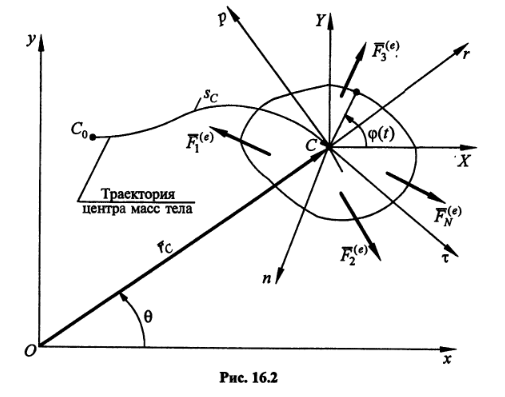
\includegraphics[scale=0.4]{img/16.2.jpeg} 
    \end{figure} 
        $$J_{CZ}\ddot{\varphi} = \sum_{k=1}^N M_{CZ}(\vec F_k^{(e)}). \quad(16.5)$$
    \par Дифференциальные уравнения (16.4) и (16.5) полностью описывают плоское движение твердого тела.Векторное уравнение (16.4) можно записать в проекциях на оси любой инерциальной системы координат. Так, в проекциях на оси Ox и Oy декартовой системы координат получаем
        $$m\ddot{x_C} = \sum_{k=1}^N F_{kx}^{(e)} ; m\ddot{y_C} = \sum_{k=1}^N F_{ky}^{(e)} . \quad(16.6)$$
    \par В проекциях на оси полярной системы координат имеем
        $$m(\ddot{r_C} - r_C \dot{\theta}^2) = \sum_{k=1}^N F_{kr}^{(e)}; m(r_C\ddot{\theta} + 2\dot{r_C}\dot{\theta}) = \sum_{k=1}^N F_{k\rho}^{(e)}, \quad(16.7)$$
    \par где $r_C$ и θ — полярные координаты центра масс тела в неподвижной системе отсчета (на рис. 16.2 полярная ось совмещена с осью Ox, а полярная координата $r_C = OC = |\vec r_C|$).
    \par Наконец, в проекциях на касательную и нормальную оси естественной системы координат уравнение (16.4) принимает следующий вид:
        $$ m\ddot{s_C} = \sum_{k=1}^N F_{k\tau}^{(e)} ; m\frac{\dot{s_c^2}}{\rho} = \sum_{k=1}^N F_{kn}^{(e)}. \quad(16.8) $$
    \par Здесь $s_C = s_C(t)$ — закон движения центра масс по траектории (на рис. 16.2 начало отсчета $S_C$ принято в точке $C_0$);  ρ — радиус кривизны траектории центра масс тела.
    \par Системы уравнений (16.5) и (16.6), (16.5) и (16.7), (16.5) и (16.8) называются дифференциальными уравнениями плоского движения твердого тела в со-ответствующей системе координат.Начальные  условия  в  общем  случае  можно  задать,  например,  так:  
    \par при $t = t_0$
        $$x_C = x_0, y_C = y_0, \varphi = \varphi_0, \dot{x_C} = \dot{x_0}, \dot{y_C} = \dot{y_0} \dot{\varphi} = \dot{\varphi_0}$$
    \par или
        $$r_C = r_0, \theta = \theta_0, \varphi = \varphi_0, \dot{r_C} = \dot{r_0}, \dot{\theta} = \dot{\theta_0}, \dot{\varphi} = \dot{\varphi_0} $$
    \par или
        $$s_C = s_0, \varphi = \varphi_0, \dot{s_c} = \dot{s_0}, \dot{\varphi} = \dot{\varphi_0}$$
    \par В зависимости от числа степеней свободы тела для описания его плоского движения можно использовать от одной до трех обобщенных координат, при необходимости выражая через них координаты, используемые в приведенных выше уравнениях и начальных условиях   
\end{center}

%19
\section{Элементарная и полная работа силы. Мощность. Работа равнодействующей силы.}
\begin{center}
    \par Изменение кинетической энергии механической системы связано с работой сил, приложенных к этой системе.
	  \par\textbf{Элементарная работа силы.} Пусть точка приложения силы $\vec F$ перемещается по криволинейной траектории из положения $M_O$ в положение $M_1$ (рис. 15.29). Разобьём перемещение точки М по дуге $M_o M_1$ на элементарные (бесконечно малые) перемещения ds и определим работу силы на каждом та-ком перемещении

	  $$d' A(\vec F) = F ds \cdot cos{\alpha}, \qquad (15.85)$$

	  \par где $\alpha$ - угол между векторами $\vec F$ и $\vec\nu$ в точке М.

     \par \begin{figure}[H]
     \centering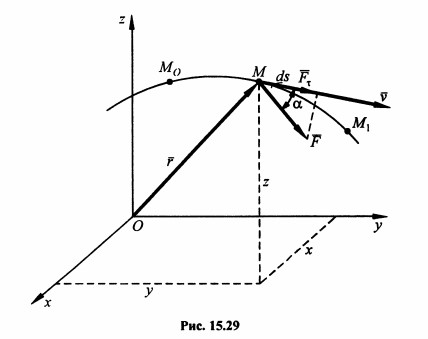
\includegraphics[scale=0.7]{img/15.29.jpg} 
     \end{figure}

	  \par Формула (15.85) определяет элементарную работу силы, обозначение d' используется для того, чтобы подчеркнуть, что выражение для элементарной работы не всегда является полным дифференциалом. Величина d'A скаляр-ная, ее знак определяется знаком  функции $\cos{\alpha}$. Если $\alpha = \frac{\pi}{2}$, то d'A = 0, если проекция силы направлена в сторону, противолежащую перемещению, то d'A < 0. Так как $F\cos{\alpha} =F_{\tau}$, то формулу (15.85) можно представить в виде

	  $$d'A = F_{\tau} ds. \qquad (15.86)$$

	  \par Таким образом, элементарная работа силы равна произведению элементарного перемещения на проекцию силы на это перемещение.
	  \par Поскольку $ds = |d \vec r|$, то согласно (15.85),

	  $$d'A = |\vec F||d \vec r| \cos{\alpha},$$
	  \par или 
	  $$d'A = \vec F \cdot d \vec r. \qquad (15.87)$$
	  
	  \par Следовательно, элементарная работа силы равна скалярному произведению векторов силы и дифференциала радиуса-вектора точки ее приложения.
	  \par Так как $d \vec r = \vec\nu dt$, представим выражение (15.87) в виде

	  $$d'A = \vec F \cdot \vec\nu dt = (\vec F dt) \cdot \vec\nu. \qquad (15.88)$$

	  \par Таким образом, элементарная работа силы равна скалярному произведению элементарного импульса силы на скорость точки ее приложения.Если скалярное произведение записать в аналитическом виде, то форму-лу (15.87) можно представить в следующем виде:

	  $$d'A = \vec F \cdot d \vec r = F_x dx + F_y dy + F_z dz.$$

	  \par\textbf{Полная работа силы.} Полную рабоу силы $\vec F$ на перемещении точки из положения $M_O$ в положение М определяют как предел суммы её элементарных работ, т.е.

	  $$A(\vec F) = \lim_{x\to \infty} \sum\limits_{k=1}^N d'A_k,$$

	  \par где $d' A_k$ - работа силы $\vec F$ на k-м элементарном перемещении, на которые разбита криволинейная дуга $M_O M$.
      \par Сумма (15.89) является интегральной суммой определения криволиней-ного интеграла, поэтому

	  $$A(\vec F) = \int\limits_{M_0}^M d'A.$$

	  \par Используя различные формулы для определения элементарной работы, получаем

	  $$A(\vec F) = \int\limits_{M_0}^M F_{\tau} ds,$$
        \par или

	  $$A(\vec F) = \int\limits_{M_0}^M \vec F d \vec r = \int\limits_{M_0}^M (F_x dx + F_y dy + F_z dz).$$

	  \par Если же сила является функцией времени, то, согласно (15.88), работа силы $\vec F$ на промежутке времени от 0 до t, соответствующем точкам $M_0$ и М, определяется выражением

	  $$A(\vec F) = \int\limits_{0}^t \vec F \cdot \vec\nu dt. \qquad (15.90)$$

	  \par Работа силы зависит от характера движения точки приложения силы. Так, A=0 , если сила приложена к неподвижной точке или к точке, скорость которой во время движения равна нулю (например, в МЦС).

	  \par\textbf{Работа равнодействующей силы.} Рассмотрим систему сил $(\vec F_1,\vec F_2,...,\vec F_N)$, приложенную к рассматриваемой точке. Эта система имеет равнодействующую $\vec R^*$, причём

	  $$\vec R^* = \vec F_1 + \vec F_2 + ... + \vec F_N.$$

	  \par Тогда работа силы $\vec R^*$ на перемещении точки из положения $M_0$ в текущее положение М равна алгебраической сумме работ составляющих сил на том же перемещении:
	  
	  $$A = \int\limits_{M_0}^M d'A = \int\limits_{M_0}^M \vec R^* d \vec r = \int\limits_{M_0}^M \vec F_1 d \vec r + \int\limits_{M_0}^M \vec F_2 d \vec r + ... + \int\limits_{M_0}^M \vec F_N d \vec r = \sum\limits_{k=1}^N A_k.$$

	  \par Единицей измерения работы в СИ является джоуль.

	  \par\textbf{Мощность.} Отношение приращения работы силы к элементарному промежутку времени, за которое оно произошло, называется мощностью:
      
      $$W = \frac{d'A}{dt}.$$

	  \par Так как $d'A = \vec F \cdot \vec\nu dt$, то

	  $$W = \vec F \cdot \vec\nu.$$

	  \par Таким образом, мощность силы равна скалярному произведению силы на скорость точки ее приложения.Единицей измерения мощности в СИ является ватт.
\end{center}
%20
\section{Работа сил, приложенных к твердому телу, при его различных движениях.}
\begin{center}
    \par \textbf{Работа  силы  при  поступательном  движении  твердого тела.}
    \par При  поступательном движении твердого тела векторы скоростей, а также элементарные перемещения всех точек тела одинаковы.
    \par Тогда элементарная работа силы
        $${dA}'(\vec{F}) = \vec F\cdot\vec v_kdt = \vec F \cdot d\vec r.$$
    \par Полная работа силы на каком-либо перемещении будет
        $$A(\vec F) = \int_{M_0}^{M} \vec F d \vec r.$$
    \par \textbf{Работа силы при вращении твердого тела вокруг неподвижной оси.} Разложим силу $\vec F$ , приложенную в произвольной точке M тела, по осям $\tau, n, b$ естественного трехгранника (рис. 15.32):
        $$\vec F = \vec F_\tau + \vec F_n + \vec F_b$$
    \par Работы составляющих силы по нормали и бинормали равны нулю, ибо они направлены всегда перпендикулярно к вектору скорости точки M приложения силы. Следовательно, элементарная работа силы $\vec{F}$  совершается только ее составляющей $F_{\tau}$ по касательной к траектории, т. е. 
        $$d'A(\vec F) = F_\tau ds$$
    \par Поскольку $\mathrm{d}s=h\mathrm{d}\phi$, то
        $$d'A(\vec F) = F_\tau hd\varphi$$
    \par где h — кратчайшее расстояние от точки приложения силы до оси вращения.
    \par Учитывая,  что $F_{\tau}h = M_z(\vec F)$  —  момент  силы  относительно  оси  Oz, получаем
        $$d'A(\vec F) = M_z(\vec F)d\varphi$$
    \par Таким  образом,  элементарная  работа  силы,  приложенной  к  какой-либо точке тела, вращающегося вокруг неподвижной оси, равна произведению момента этой силы относительно оси вращения на дифференциал угла поворота тела.
    \par Полная работа
        $$A(\vec F) = \int_{0}^{\varphi} M_z(\vec F) d \varphi.$$
    \par В  случае,  когда  момент  силы  относительно  оси  вращения  тела  постоянен, полная работа $A=M_z\varphi$.
    \par Мощность силы в рассматриваемом случае
        $$W = \frac{d'A}{dt} = \frac{M_z(\vec F)d\varphi}{dt} = M_z(\vec F)\omega_z$$
    \par $\omega_z = \frac{\mathrm{d}\varphi}{\mathrm{d}t}$  — проекция на ось Oz угловой скорости тела.
    \par \textbf{Работа силы в общем случае движения свободного твердого тела.} Скорость точки M приложения силы $\vec F$  (рис. 15.33) в рассматриваемом случае равна
        $$\vec v = \vec v_A + \vec \omega \times \vec r$$
    \par где  $\vec v_A$ — скорость полюса A;  $\vec r = \vec{AM}$. Тогда
        $$d'A(\vec F) = \vec F \cdot \vec vdt = \vec F \cdot \vec v_Adt + \vec F \cdot (\vec \omega \times \vec r)dt$$
        
    %рисунок 15.33
    \par \begin{figure}[H]
        \centering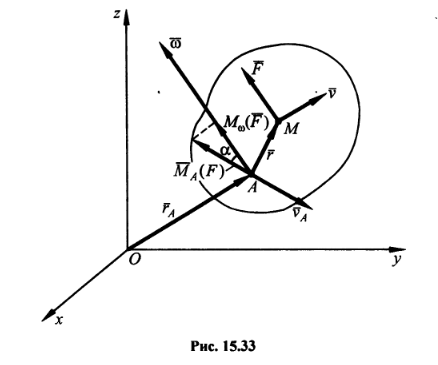
\includegraphics[scale=0.5]{img/15.33.jpeg} 
    \end{figure}
        
    \par Так как
        $$\vec v_A dt = d \vec r_A, \vec F \cdot (\vec \omega \times \vec r) = \vec \omega \cdot (\vec r \times \vec F) = \vec \omega \cdot \vec M_A(\vec F), $$
    \par то 
        $$d'A(\vec F) = \vec F \cdot d \vec r_A + \omega \cdot \vec M_A (\vec F) dt$$
    \par или
        $$d'A(\vec F) = \vec F \cdot d \vec r_A + \vec M_\omega (\vec F) d \varphi$$
    \par где $M_{\omega}(\vec F)$ — проекция $\vec M_A(\vec F)$ на вектор  $\vec \omega$; $\mathrm{d}\varphi$  — элементарный угол поворота тела вокруг мгновенной оси относительного вращения.Таким образом, элементарная работа силы, приложенной в какой-либо точке твердого тела, в общем случае его движения равна сумме элементарных работ на элементарном поступательном перемещении вместе с полюсом и элементарном вращательном перемещении вокруг мгновенной оси, проходящей через полюс.
\end{center}
%21
\section{Кинетическая энергия точки и системы материальных точек. Теорема Кёнига.}
\begin{center}
    \par Кинетическая энергия точки и системы. Кинетическую энергию материальной точки массой m, движущейся с абсолютной скоростью v, определяют по формуле
    \par $T= \frac{mv^2}{2}$, где $v^2=v^{-2}$
    \par Кинетическая энергия механической системы равна сумме кинетических энергий всех точек этой системы:
    \par $ T = \sum_{k=1}^N {\frac{m_kv_k^2}{2}} \qquad$ (15.78)
    \par Кинетическая энергия — положительная скалярная величина. Единицей измерения кинетической энергии в СИ является джоуль.
    \par Рассмотрим движение механической системы в неподвижной системе отсчета Oxyz  (рис. 15.27). В качестве подвижной выберем систему  CXYZ  с началом в центре масс — точке C, движущуюся поступательно вместе  с  центром  масс.  Абсолютное  движение  механической  системы  при этом можно рассматривать как совокупность переносного (вместе с центром масс) и относительного (по отношению к центру масс) движений системы.Для любого момента времени положение произвольной точки $M_k$ системы по отношению к неподвижному центру O определяет радиус-вектор
    \par $\vec{r_k} = \vec{r_c} + \vec {\rho_k}$
    \par где $\vec{\rho_k}$  —  радиус-вектор  точки $M_k$  по  отношению  к  центру  масс  C  (см. рис.  15.27).  Продифференцировав это равенство  по  времени,  найдем  абсолютную скорость произвольной точки системы
    \par $\vec{v_k} = \vec{v_c} + \vec {v}_k^{(r)}$
    \par где  $ \vec {v}_k^{(r)} = \frac{d \vec{\rho}_k}{dt} $  — относительная скорость точки (в данном случае полная производная по времени от $ \vec{\rho}_k$ равна локальной, так как система  CXYZ  движется поступательно, т. е. $ \vec{\omega}_e=0 $).
    \begin{figure}[H]
        \centering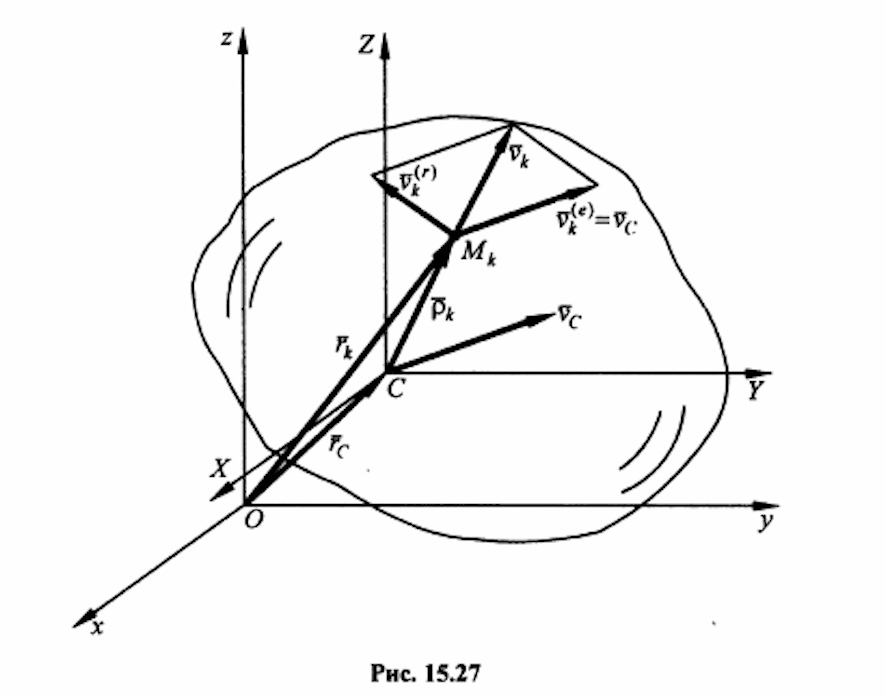
\includegraphics[scale=0.25]{img/15.27.jpeg} 
    \end{figure}
    \par Учитывая, что квадрат вектора равен квадрату его модуля, преобразуем выражение (15.78) к виду 
    \par $T = \frac{1}{2} \sum_{k=1}^N {m_k v_k^2} = \frac{1}{2} \sum_{k=1}^N {m_k \vec{v}_k^{-2}} =  \frac{1}{2} \sum_{k=1}^N {m_k \vec{v}_c^2} + \sum_{k=1}^N {m_k \vec{v}_c \vec{v}_k^{(r)}} + \frac{1}{2} \sum_{k=1}^N {m_k (\vec{v}_k^{(r)})^2} $
    \par Здесь 
    \par $\sum_{k=1}^N {m_k \vec{v}_c \vec{v}_k^{(r)}} = \vec{v}_c \sum_{k=1}^N {m_k \vec{v}_k^{(r)}} = \vec{v}_c \sum_{k=1}^N {m_k \frac{d \vec{\rho}_k}{dt}} = \vec{v}_c \frac{d}{dt}(\sum_{k=1}^N {m_k \vec{\rho}_k}) = 0 $
    \par поскольку сумма статических моментов масс точек относительно центра масс $\sum_{k=1}^N {m_k \vec{\rho}_k=0} $
    \par Таким образом, 
    \par $ T= \frac{1}{2} M v_C^2 + \frac{1}{2} \sum_{k=1}^N{m_k (v_k^{(r)})^2} \qquad$ (15.79),
    \par где  $ M= \sum_{k=1}^N {m_k} $ - масса механической системы.
    \par Формула (15.79) выражает теорему Кенига: кинетическая энергия механической системы в ее абсолютном движении равна сумме кинетической энергии центра масс, в предположении, что в нем сосредоточена масса всей системы, и кинетической энергии движения системы относительно центра масс.
\end{center}
%22
\section{Кинетическая энергия твердого тела в различных случаях его движения.}
\begin{center}
    \par \textbf{При поступательном движении твердого тела} скорости всех его точек одинаковы и равны скорости центра масс, поэтому 
    
    \par $T=\sum_{k=1}^{N}\frac{m_{k}\nu_{k}^{2}}{2} = \sum_{k=1}^{N}\frac{m_{k}\nu_{c}^{2}}{2} = \frac{\nu_{c}^{2}}{2}\sum_{k=1}^{N}m_{k} = \frac{1}{2}M\nu_{c}^{2}$, где M - масса твёрдого тела.
    
    \par \textbf {При  вращении  твердого  тела  вокруг  неподвижной  оси} скорость его произвольной точки. 
    
    \par $ \nu_{k} = \omega h_{k}$, где $ {h_{k}} $ — кратчайшее расстояние от точки $ {M_{k}} $ до оси вращения.
    
    \par Тогда $ T= \frac{1}{2}\sum_{k=1}^{N}{m_{k}\nu_{k}^{2}}= \frac{\omega^{2}}{2}\sum_{k=1}^{N}m_{k}h_{k}^{2} = \frac{1}{2}J_{z}\omega^{2} $, 
    \par где $J_{z} = \sum_{k=1}^{N}m_{k}h_{k}^{2}$ — момент инерции тела относительно оси вращения ${O_{z}}$.
   
    \par \textbf{При плоском движении твердого тела,} которое можно рассматривать как совокупность поступательного движения вместе с центром масс C и вращения  вокруг  подвижной  оси  ${C_{z}}$,  движущейся  поступательно  вместе  с центром масс, относительная скорость произвольной точки тела ${ \nu_{k}^{r} = \omega H_{k}}$, и, следовательно, согласно формуле Кенига,
    $T = \frac{1}{2}M\nu_{C}^{2} + \frac{1}{2}J_{CZ}\omega$, где ${C_{CZ}}$ — момент инерции тела относительно оси ${C_{Z}}$.

    \par \textbf {При сферическом движении твердого тела} скорость произвольной точки определяется формулой Эйлера
    \par $ \vec{\nu_{k}} = \omega \times\vec{r_{k}}. $
    
    \par $ T= \sum_{k=1}^{N} \frac{m_{k} \vec{\nu}^{2}}{2} = \frac{1}{2}\sum_{k=1}^{N}m_{k}\vec{\nu_{k}}(\vec{\omega} \times \vec{r_{k}}) = \frac{1}{2}\sum_{k=1}^{N}\vec{\omega}(\vec{r_{k}} \times m_{k}\vec{\nu_{k}} )=\frac{1}{2}\vec{\omega}\sum_{k=1}^{N} \vec{r_{k}} \times m_{k}\vec{\nu_{k}} =\frac{1}{2}\vec{\omega}\vec{K_{0}} $

    \par где $ K_{0} = \sum_{k=1}^{N} \vec{r_{k}} \times m_{k}\vec{\nu_{k}}  $- главный момент количеств движения системы относительно неподвижной точки 0.

    \par \textbf {В  общем  случае  движения  свободного  твердого  тела  в  пространстве}, которое можно рассматривать как совокупность поступательного переносного движения вместе с центром масс и сферического движения по отношению к этому центру (рис.15.28), относительная скорость произвольной точки тела $\vec{\nu_{k}^{(r)}} = \vec{\omega} \times \vec{\rho_{k}} $ , кинетическая энергия тела $ T = \frac{1}{2}M\nu^{2}_{C} + \frac{1}{2} \vec{\omega}\vec{K}_{C}^{(r)}$
    \par Где ${ \vec{K}_{C}^{(r)} } $ — главный момент количеств относительного движения относительно центра масс.
    \begin{figure}[H]
    \centering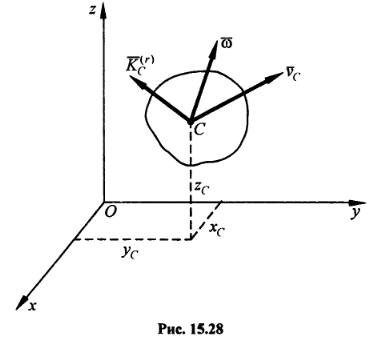
\includegraphics[scale=0.5]{img/15.28.jpeg} 
    \end{figure}

    \par Таким  образом,  в  данном  случае  кинетическая  энергия  твердого  тела определяется как сумма кинетической энергии тела в его переносном поступательном движении вместе с центром масс и кинетической энергии тела в сферическом движении относительно центра масс.
\end{center}
%23
\section{Теорема об изменении кинетической энергии для точки и системы материальных точек.}
\begin{center}
    \par Кинетическая энергия твердого тела. При поступательном движении твердого тела скорости всех его точек одинаковы и равны скорости центра масс, поэтому
    \par $T= \sum_{k=1}^{N} {\frac{m_k v_k^2}{2}} = T= \sum_{k=1}^{N}{\frac{m_k v_C^2}{2}} = \frac{v_C^2}{2} \sum_{k=1}^{N} {m_k} = \frac{1}{2} M v_C^2 $
    \par где M - масса твердого тела 
    \par При  вращении  твердого  тела  вокруг  неподвижной  оси  скорость его произвольной точки
    \par $ v_k = \omega h_k$
    \par где $ h_k$ - кратчайшее расстояние от точки $M_k$ до оси вращения 
    \par Тогда 
    \par $T= \sum_{k=1}^{N} {\frac{m_k v_k^2}{2}} = \frac{\omega^2}{2} \sum_{k=1}^{N} {m_k h_k^2} = \frac{1}{2} J_z \omega^2  $
    \par где $J_z = \sum_{k=1}^{N} {m_k h_k^2}$ - момент инерции тела относительно оси вращения Oz 
    \par При плоском движении твердого тела, которое можно рассматривать как совокупность поступательного движения вместе с центром масс C и вращения  вокруг  подвижной  оси  CZ,  движущейся  поступательно  вместе  с центром масс, относительная скорость произвольной точки тела $ v_k^{(r)} = \omega h_k$, и, следовательно, согласно формуле Кенига,
    \par $T = \frac{1}{2} M v_c^2 + \frac{1}{2} J_{CZ} \omega^2 $
    \par $J_CZ$ - момент инерции относительно оси CZ.
    \par При  сферическом  движении  твердого  тела скорость произвольной точки определяется формулой Эйлера
    \par $\Vec{v}_k = \vec{\omega} \times {\vec{r}_k} \qquad$ (15.80)
    \par Преобразуем формулу (15.78) с учетом выражения (15.80)
    \par $ \frac{1}{2} \sum_{k=1}^N {m_k \vec {v}_k^2} = \frac{1}{2} \sum_{k=1}^N {m_k v_k (\vec{\omega} \times {\vec{r}_k})} =\frac{1}{2} \sum_{k=1}^N {\vec{\omega} (\vec{r}_k \times m_k \vec{v}_k)} = \frac{1}{2} \vec{\omega} \sum_{k=1}^N {\vec{r}_k \times m_k \vec{v}_k} = \frac{1}{2} \vec{\omega} \vec{K}_O \qquad$ (15.81)
    \par Здесь $\vec{K}_O = \sum_{k=1}^N {\vec{r}_k \times m_k \vec{v}_k}$ -главный момент количества движения системы относительно неподвижной точки О.
    \par С учетом (15.46) кинетическую энергию твердого тела при сферическом движении (15.81) можно представить в виде
    \par $ T = \frac{1}{2} [\omega_x (J_x \omega_x - J_{xy} \omega_y - J_{xz} \omega_z) + \omega_y(-J_{xy}\omega_x + J_y \omega_y - J_{yz}\omega_z) + \omega_z (-J_{xz} \omega_x - J_{yz} \omega_y + J_z \omega_z)]  \qquad$ (15.82)
    \par где  $J_x, J_y, ..., J_{yz} $ -— осевые и центробежные моменты инерции твердого тела в системе координат Oxyz  (см. гл. 14).
    \par Если оси системы координат  Oxyz  направить по главным осям инерции тела для точки O, то, согласно формулам (15.47), выражение (15.82) примет вид
    \par $T = \frac{1}{2} (J_x \omega_x^2 + J_y \omega_y^2 + J_z \omega_z^2) \qquad$ (15.83)
    \par В  общем  случае  движения  свободного  твердого  тела  в  пространстве, которое можно рассматривать как совокупность поступательно-го переносного движения вместе с центром масс и сферического движения по отношению к этому центру (рис. 15.28), относительная скорость произвольной точки тела $ \vec{v}_k^{(r)}= {\vec{\omega} \times \vec{\rho}_k}$ и, следовательно, согласно (15.79) и (15.81), кинетическая энергия тела 
    \par $T =  M v_c^2 + \frac{1}{2} \vec{\omega} \vec{K}_c^{(r)} \qquad$ (15.84) 
    \par Здесь  $\vec{K}_c^{(r)}$ — главный момент количеств относительного движения относительно центра масс. Отметим, что для кинетической энергии относительного (сферического вокруг центра масс) движения тела несложно получить формулы типа (15.82), (15.83).
     \begin{figure}[H]
        \centering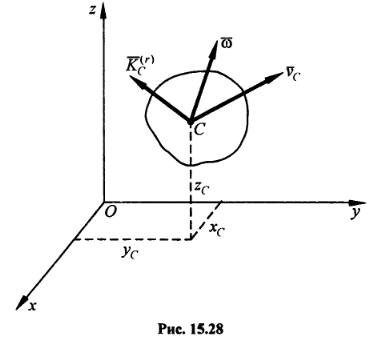
\includegraphics[scale=0.5]{img/15.28.jpeg} 
    \end{figure}
    \par Таким  образом,  в  данном  случае  кинетическая  энергия  твердого  тела определяется как сумма кинетической энергии тела в его переносном поступательном движении вместе с центром масс и кинетической энергии тела в сферическом движении относительно центра масс.
\end{center}
%24
\section{Потенциальное силовое поле. Силовая функция и потенциальная энергия поля.}
\begin{center}
    \par \textbf{Силовым полем} называется часть пространства, в котором на материальную точку действует сила, зависящая от координат точки и времени:$ \Vec{F} = \Vec{F} (x,y,z,t)$
    
    \par Если  сила  явно  не  зависит  от  времени,  то  силовое  поле  называется \textbf{стационарным}.

    \par Стационарное силовое поле называется \textbf{потенциальным}, если проекции силы F на оси ${ Ox, Oy, Oz }$ можно выразить через скалярную функцию ${U(x, y, z)}$ по формулам 

    \par $ F_{x} = \frac{\partial{U}}{\partial{x}};  F_{y} = \frac{\partial{U}}{\partial{y}};  F_{z} = \frac{\partial{U}}{\partial{z}},$ \qquad (15.100)

    \par т.е. $ \Vec{F} = \vec{grad}U $, где $\vec{grad}U = \frac{\partial{U}}{\partial{x}} \vec{i} + \frac{\partial{U}}{\partial{y}} \vec{j} + \frac{\partial{U}}{\partial{z}} \vec{k} $

    \par Функция  ${U(x,  y,  z)}$  называется  \textbf{силовой  функцией}.  Из  формул  (15.100) следует,  что  силовая  функция  U  определяется  с  точностью  до  аддитивной постоянной.

    \par \textbf{Свойства стационарного потенциального поля}

    \par 1. Элементарная работа силы стационарного потенциального поля равна полному дифференциалу силовой функции:

    \par $d'A = \vec{F}d\vec{r} = F_{x}dx + F_{y}dy+F_{z}dz =\frac{\partial{U}}{\partial{x}} dx + \frac{\partial{U}}{\partial{y}} dy + \frac{\partial{U}}{\partial{z}} dz = dU. $ \qquad (15.101)
    \par 2. Полная работа силы стационарного потенциального поля не зависит от траектории, по которой перемещается точка, и определяется лишь начальным и конечным положением точки:

    \par $A=\int_{M_{0}}^{M}d'A=\int_{M_{0}}^{M}dU=U(x,y,z)-U(x_{0},y_{0},z_{0}).$ \qquad (15.102)

    \par 3.Работа силы $ \vec{F}$  стационарного потенциального поля по любому замкнутому перемещению равна нулю (см. (15.102)), так как значение силовой функции в начальной и конечной точках одинаковы (если внутри замкнутого контура нет особых точек силовой функции), т. е.

    \par $\oint \vec{F}d\vec{r} = 0.$

    \par 4. Для того чтобы стационарное силовое поле было потенциальным, необходимо и достаточно, чтобы поле было безвихревым, т. е. сила $\vec{F}$ удовлетворяла условиям:

    \par $ \frac{\partial F_{Z}}{\partial y} - \frac{\partial F_{y}}{\partial z} = 0; \frac{\partial F_{x}}{\partial z} - \frac{\partial F_{z}}{\partial x} = 0; \frac{\partial F_{y}}{\partial x} - \frac{\partial F_{x}}{\partial y} = 0. $ \qquad (15.103)
    
    \par Если использовать вектор вихря

    \par $rot\vec{F} =(\frac{\partial F_{z}}{\partial y} - \frac{\partial F_{y}}{\partial z} )\vec{i} + (\frac{\partial F_{x}}{\partial z} - \frac{\partial F_{z}}{\partial x})\vec{j} +(\frac{\partial F_{y}}{\partial x} - \frac{\partial F_{x}}{\partial y})\vec{k},$

    \par то условия (15.103) можно записать короче:
    \par $rot\vec{F} = 0.$
    
    \par \textbf{Потенциальной энергией} материальной точки в данной точке потенциального силового поля называют работу, производимую силой, действующей на точку в потенциальном силовом поле, при ее перемещении из рассматриваемой точки поля M в начальную $M_{0}$, условно принимаемую за нулевую:

    \par $ \Pi = A_{MM_{0}} = \int_M^{M_{0}}dU = U(M_{0}) - U(M).$ Поскольку $U(M_{0}) = C_{0} $ ,то $ \Pi = C_{0} - U,$ \qquad (15.104)

    \par т.е. потенциальная энергия в какой-либо точке поля с точностью до произвольной постоянной $C_{0}$ равна  силовой  функции в  той же  точке,  взятой со знаком минус. На основании формул (15.100), (15,101), (15.104) имеем

    \par $  F_{x} = \frac{\partial{U}}{\partial{x}} = -\frac{\partial{\Pi}}{\partial{x}}; F_{y} = \frac{\partial{U}}{\partial{y}} = -\frac{\partial{\Pi}}{\partial{y}}; F_{z} = \frac{\partial{U}}{\partial{z}} = -\frac{\partial{\Pi}}{\partial{z}}; $

    \par $d'A = dU = -d\Pi, A=U-U_{0}=\Pi_{0} - \Pi, $

    \par где $U_{0}, \Pi_{0}$ — произвольные постоянные, равные значениям силовой функции и потенциальной энергии в начальной точке.
    
\end{center}
%25
\section{Поверхности уровня и их свойства.}
\begin{center}
    \par Поверхность $U(x,y,z) = C, $ \qquad (15.105)

    \par на которой силовая функция U имеет постоянное значение, называется \textbf{ поверхностью уровня}. Для конкретного поля эти поверхности образуют семейство поверхностей с параметром C; задавая C разные значения, можно получать разные поверхности уровня, которые в случае, когда функция U однозначна, не пересекаются и разделяют потенциальное поле на слои.
    
    \par \textbf{Свойства поверхностей уровня}

    \par 1. Если начальная и конечная точки расположены на одной и той же поверхности уровня, то работа силы стационарного потенциального поля по перемещению материальной точки из начального положения в конечное равна нулю. Действительно, из формулы (15.102) и определения поверхности уровня (15.105(в предыдущем вопросе)) следует

    \par $A=U(x,y,z) - U(x_{0},y_{0},z_{0}) = 0,$
    \par так как $U(x,y,z) = U(x_{0},y_{0},z_{0}) = C_{0}$ (начальная и конечная точки расположены на одной и той же поверхности уровня).

    \par 2. Сила $\vec{F}$ потенциального поля направлена по нормали к поверхности уровня в сторону возрастания силовой функции U.
\end{center}
%26
\section{Примеры вычисления силовых функций однородного поля силы тяжести и линейной силы упругости.}
\begin{center}
    \par \textbf{Однородное поле силы тяжести}

    \par Рассмотрим материальную точку массой m, находящуюся в однородном поле силы тяжести. Направим ось Oz вертикально вверх, а оси Ox и Oy произвольно в горизонтальной плоскости (рис. 15.35).Проекции силы тяжести $\vec{P} = m\vec{g}$  на оси координат будут равны

    \par $P_{x} =0;P_{y} =0;P_{z} = -mg$
    
    %картинка 15.35%
    \begin{figure}[H]
    \centering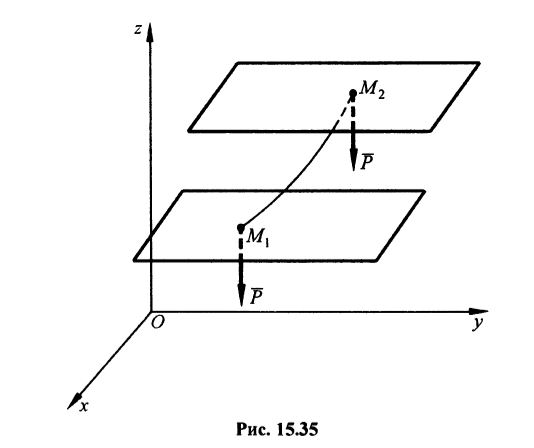
\includegraphics[scale=0.5]{img/15.35.JPG} 
    \end{figure}

    \par Элементарная работа силы тяжести

    \par $d'A = P_{x}dx + P_{y}dy + P_{z}dz = -mgdz = d(-mgz). $ \qquad (15.107)
   
    \par Поскольку элементарная работа силы тяжести является полным дифференциалом и $ d'A = dU=-d\Pi$ , то, интегрируя (15.107), находим

    \par $U=-mgz+C_{1}; \Pi = mgz +C_{2}; A=\int_{M_{1}}^{M_{2}}(P_{x}dx + P_{y}dy + P_{z}dz) = -mg\int_{z_{1}}{z_{2}}dz=-mg(z_{2}-z_{1}),$  \qquad (15.108)
    
    \par где A - работа силы тяжести материальной точки массой m на перемещении $M_{1}M_{2}$.
    
    \par Уравнение (15.108) можно представить в виде
    
    \par $A=-mgH,$ где $H=x_{2} -z_{1}$ - высота подъема точки.
    
    \par Если точка  $M_{1}$ расположена выше точки  $M_{2}$, т. е. при движении точка опускается, то работа силы тяжести положительная, в противном случае — отрицательная. Таким образом,
    
    \par $A=\pm mgh,$  \qquad (15.109) 
    \par где знак "+" соответствует перемещению точки вниз, а знак - перемещению вверх.

    \par Как следует из формулы (15.109), работа силы тяжести не зависит от формы траектории, по которой перемещается точка приложения силы. Работа силы тяжести равна нулю, если точки $M_{1}$ и $M_{2}$ совпадают (траектория — замкнутый  контур)  или  расположены  в  одной  и  той  же  горизонтальной плоскости.

    \par \textbf{Поле линейной силы упругости}

    \par Линейная сила упругости (рис. 15.36) подчиняется закону Гука: $\Vec{F} = -c\vec{r} $, где c — коэффициент упругости; r — радиус-вектор точки M, отсчитываемый от точки равновесия, где сила равна нулю.
    
    %картинка 15.36%
    \begin{figure}[H]
    \centering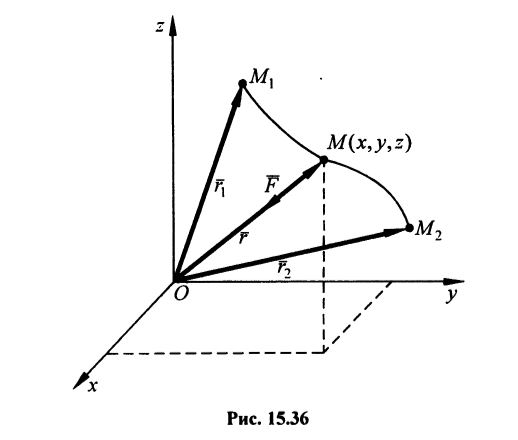
\includegraphics[scale=0.5]{img/15.36.JPG} 
    \end{figure}
    
    \par Элементарная работа этой силы $ d'A =\vec{F} d\vec{r} = -c\vec{r}d\vec{r} = d(-\frac{cr^{2}}{2})$  \qquad (15.110)
    
    \par так как $\vec{r}d\vec{r} = d \frac{1}{2}(\vec{r}^{2}) = rdr.$ Интегрируя (15.110), находим 

    \par $U = -\frac{cr^{2}}{2} + C_{1}; \Pi = \frac{cr^{2}}{2} + C_{2}; A = \int_{M_{1}}^{M_{2}}(-crdr)=-c\int_{r_{1}}^{r_{2}}rdr = -\frac{1}{2}(r_{2}^{2} - r_{1}^{2}),$  \qquad (15.111)

    \par т.е. $ U = -\frac{c}{2}(x^{2} + y^{2} +z^{2}) +C_{1}, \Pi = \frac{c}{2}(x^{2} + y^{2} +z^{2}) +C_{2}$

    \par Таким  образом,  силовая  функция  и  потенциальная  энергия  линейной  силы упругости является квадратичной формой координат точки M, отсчитываемых от положения равновесия.
    \par Как следует из  формулы (15.111),  работа  силы упругости не  зависит от формы траектории,  по которой перемещается  точка. При  перемещении же точки из положения равновесия работа силы упругости будет отрицательной:
    \par $ A=-\frac{c}{2}r^{2}$
    
    
\end{center}
%27
\section{Закон сохранения полной механической энергии системы.}
\begin{center}
    \par Пусть все силы (как внешние, так и внутренние), действующие на механическую систему, потенциальны, т. е. существует функция $U(x_{1}, y_{1},z_{1},...,x_{N},y_{N},z_{N})$ такая, что   

    \par $ F_{kx} = \frac{\partial U}{\partial x_{k}}; F_{ky} = \frac{\partial U}{\partial y_{k}}; F_{kz} = \frac{\partial U}{\partial z_{k}}; $ \qquad (15.112)

    \par где $F_{kx}\vec{i} + F_{ky}\vec{j} + F_{kz}\vec{k} = \vec{F_{k}}$ 

    \par — равнодействующая всех сил, приложенных к k-й точке.

    \par Теорему об изменении кинетической энергии системы в дифференциальной форме представим в виде

    \par $dT = \sum_{k=1}^{N}\vec{F}_{k}d\vec{r}_{k}$ , где $\vec{F}_{k} d\vec{r}_{k} = ( \vec{F}_{k}^{e} + \vec{F}_{k}^{i} )d\vec{r}_{k} $ \qquad (15.113)

    \par Так как, согласно (15.112), $ \sum_{k=1}^{N} \vec{F}_{k}d\vec{r}_{k} =\sum_{k=1}^{N}(F_{kx}dx_{k} + (F_{ky}dy_{k} +(F_{kz}dz_{k} )= \sum_{k=1}^{N}(\frac{\partial U}{\partial x_{k}}dx_{k} + \frac{\partial U}{\partial y_{k}}dy_{k} + \frac{\partial U}{\partial z_{k}}dz_{k} ) = dU$,

    \par то уравнение (15.113) примет вид

    \par $dT=dU$ или $dT + d\Pi = 0$,

    \par $\Pi = -U(x_{1}, y_{1},z_{1},...,x_{N},y_{N},z_{N}) + const $ - потенциальная энергия системы.

    \par Следовательно, $d(T+\Pi)=0,$ отсюда получаем $T+\Pi = const$ и $E=T+\Pi =T_{0} + \Pi_{0}=const$ \qquad (15.114)

    \par Сумма кинетической и потенциальной энергии называется \textbf{полной энергией E} механической системы. Системы, для которых выполняется закон сохранения механической энергии, называются \textbf{консервативными.}

    \par Формула (15.114) выражает закон сохранения механической энергии для механической системы: \textbf{если все силы, действующие на систему, потенциальны, то при движении системы ее полная механическая энергия постоянна.}
    
    \par Следует отметить, что закон сохранения механической энергии справедлив и в том случае, когда кроме потенциальных имеются и непотенциальные силы, но которые при движении системы не совершают работы. 
    
\end{center}

%28
\section{Принцип Даламбера для точки и системы материальных точек. Сила инерции материальной точки. Главный вектор и главный момент сил инерции в общем и частных случаях движения твердого тела. Метод кинетостатики.}
\begin{center}
    \par В  соответствии  с  аксиомами  динамики  основное  уравнение  движения материальной точки имеет вид

	  $$m \vec a = \vec F + \vec R, \qquad (17.1)$$

	  \par где $\vec F$ - равнодействующая активных сил; $\vec R$ - равнодействующая реакций связей; $\vec a = \frac{d^2 \vec r}{d t^2}$ - абсолютное ускорение точки.

	  \par Уравнение (17.1) можно также записать в виде

	  $$\vec F + \vec R + (-m \vec a) = 0$$

	  \par Слагаемое $(-m \vec a)$ обозначают $\vec\Phi$ и называют \textbf{даламберовой силой инерции} (или просто силой инерции). Основное уравнение динамики материальной точки при использовании силы инерции принимает следующий вид:
	  
	  $$\vec F + \vec R + \vec\Phi = 0. \qquad (17.2)$$

	  \par Так как указанные выше силы образуют систему сходящихся сил, то урав-нение  (17.2)  можно  рассматривать  как  условие  равновесия  системы  сил $(\vec F, \vec R, \vec\Phi)$. В  этом  и  состоит  принцип  Даламбера  для  материальной  точки. Формулируется он так: при движении материальной точки в любой момент времени приложенные к ней активные силы и реакции связей вместе с силой инерции образуют систему сил, эквивалентную нулю (уравновешенную систему сил), т. е.
	  
	  $$(\vec F, \vec R, \vec\Phi) \sim 0. \qquad (17.3)$$

	  \par Отметим, что в формулировке принципа Даламбера речь идет об уравновешенности определенной системы сил, а не о равновесии (покое) материальной точки. Таким образом, дополняя систему активных сил и реакций связей, приложенных к точке, силой инерции, получаем уравновешенную систему сходящихся сил, для которой должно выполняться условие равновесия (17.2). В проекциях на оси декартовой системы координат имеем

	  $$ F_x + R_x + \Phi_x = 0; \quad  F_y + R_y + \Phi_y = 0; \quad F_z + R_z + \Phi_z = 0,$$

	  \par где $\Phi_x = -m \ddot x; \quad \Phi_y = -m \ddot y; \quad \Phi_z = -m \ddot z$; в проекциях на оси естественной системы координат получаем

	  $$ F_{\tau} + R_{\tau} + \phi_{\tau} = 0; \quad F_{n} + R_{n} + \phi_{n} = 0; \quad F_b + R_b = 0,$$

	  \par где $ \Phi_{\tau} = -m a_{\tau} = -m \frac{d \nu_{\tau}}{dt}; \quad \Phi_{n} = -m a_n = -m \frac{\nu^2}{\rho}$.
        \par\textbf{Принцип даламбера для механической системы}

	  \par Рассмотрим механическую систему,  состоящую  из  N материальных  точек. Применяя принцип Даламбера к каждой точке системы, получаем

	  $$ \vec F_k + \vec R_k + \vec\Phi_k = 0, k = 1,2,...,N, \qquad (17.4)$$

	  \par где $ \vec\Phi_k = -m_k \vec a_k; quad \vec F_k$ и $\vec R_k$ — равнодействующие активных сил и реакций связей, приложенных к k-й точке. Условие (17.4) можно представить в виде
	  
	  $$(\vec F_k, \vec R_k, \vec\Phi_k) \sim 0, \quad k=1,2,...,N.$$

	  \par Таким  образом,  для  системы  материальных  точек  принцип  Даламбера формулируется так: при движении механической системы в любой момент времени приложенные к  каждой  точке системы активные силы  и  реакции связей вместе с силами инерции образуют систему сил, эквивалентную нулю. Суммируя левые части уравнений (17.4) по всем точкам системы, получаем

	  $$ \sum\limits_{k=1}^N \vec F_k + \sum\limits_{k=1}^N \vec R_k + \sum\limits_{k=1}^N \vec\Phi_k = 0. \qquad (17.5)$$

	  \par Умножив каждое уравнение в (17.4) векторно слева на радиус-вектор $\vec r_k$ k-й точки и просуммировав их, имеем
     
	  $$ \sum\limits_{k=1}^N \vec r_k \times \vec F_k + \sum\limits_{k=1}^N \vec r_k \times \vec R_k + \sum\limits_{k=1}^N \vec r_k \times \vec\Phi_k = 0,$$

	  \par или

	  $$ \sum\limits_{k=1}^N \vec M_O (\vec F_k) + \sum\limits_{k=1}^N \vec M_O (\vec R_k) + \sum\limits_{k=1}^N \vec M_O (\vec\Phi_k) = 0. \qquad (17.6)$$

	  \par Из (17.5) и (17.6) следует, что равны нулю главный вектор и главный момент  относительно  произвольного  центра  приведения O активных сил, реакций  связей,  приложенных  ко  всем  точкам  механической  системы,  и  сил инерции. В проекциях на оси декартовой системы координат, начало которых совпадает с центром O, эти условия принимают вид известных уравнений равновесия произвольной пространственной системы сил:

        \par$ \sum\limits_{k=1}^N F_{kx} + \sum\limits_{k=1}^N R_{kx} + \sum\limits_{k=1}^N \Phi_{kx} = 0$;
	  \par$ \sum\limits_{k=1}^N F_{ky} + \sum\limits_{k=1}^N R_{ky} + \sum\limits_{k=1}^N \Phi_{ky} = 0$;
	  \par$ \sum\limits_{k=1}^N F_{kz} + \sum\limits_{k=1}^N R_{kz} + \sum\limits_{k=1}^N \Phi_{kz} = 0; \qquad (17.7)$
	  \par$ \sum\limits_{k=1}^N M_x (\vec F_k) + \sum\limits_{k=1}^N M_x (\vec R_k) + \sum\limits_{k=1}^N M_x (\vec\Phi_k) = 0$;
	  \par$ \sum\limits_{k=1}^N M_y (\vec F_k) + \sum\limits_{k=1}^N M_y (\vec R_k) + \sum\limits_{k=1}^N M_y (\vec\Phi_k) = 0$;
	  \par$ \sum\limits_{k=1}^N M_z (\vec F_k) + \sum\limits_{k=1}^N M_z (\vec R_k) + \sum\limits_{k=1}^N M_z (\vec\Phi_k) = 0$.

	  \par Если силы, приложенные к k-й точке системы, разложить не на активные и реакции связей, а на внешнюю $\vec F_k^e$, и внутреннюю $\vec F_k^i$, то уравнение (17.4) принимает вид

        $$ \vec F_k^{(e)} + \vec F_k^{(i)} + \vec\Phi_k = 0.$$
        \par Поскольку главный вектор и главный момент относительно произвольного центра приведения внутренних сил системы равен нулю, то для (17.5) и (17.6) имеем соответственно

	  $$ \sum\limits_{k=1}^N \vec F_k^{(e)} + \sum\limits_{k=1}^N \vec\Phi_k = 0; \quad \sum\limits_{k=1}^N \vec M_O (\vec F_k^{(e)}) + \sum\limits_{k=1}^N \vec M_O (\vec\Phi_k) = 0. \qquad (17.8)$$

	  \par Проецируя  (17.8)  на  оси  декартовой  системы  координат,  получаем  шесть уравнений  равновесия  системы  сил,  аналогичных  уравнениям  (17.7).  Особенность этих уравнений состоит в том, что в них не входят внутренние силы.
	  \par Понятие о силе инерции и принцип Даламбера составляют основу метода кинетостатики, который ставит своей целью применение методов статики, в частности, к задачам динамики машин и механизмов.
        \par\textbf{Главный вектор и главный момент сил инерции}

	  \par Применяя принцип Даламбера для изучения движения механических систем, состоящих из многих или множества (например, твердое тело) точек, силы инерции целесообразно привести к какому-либо центру, например центру масс. Получим общие формулы для главного вектора и главного момента сил инерции относительно произвольно выбранного центра приведения.

	  \par\textbf{Главный вектор сил инерции}

	  \par В соответствии с определением главного вектора

	  $$ \vec R_{UH} = \sum\limits_{k=1}^N \vec\Phi_k = - \sum\limits_{k=1}^N m_k \vec a_k.$$

	  \par Так как ускорение точки $ \vec a_k = \frac{d^2 \vec r_k}{d t^2}$, а её масса $m_k$ постоянна, то

	  $$ \vec R_{UH} = -\frac{d^2}{d t^2} (\sum\limits_{k=1}^N m_k \vec r_k) = -M \frac{d^2}{d t^2} (\frac{\sum\limits_{k=1}^N m_k \vec r_k}{M}) = -M \frac{d^2 \vec r_C}{d t^2}.$$

	  \par Таким  образом,  при  любом  движении  механической  системы  главный вектор сил инерции равен взятому со знаком «минус» произведению массы системы на ускорение центра масс:

	  $$ \vec R_{UH} = -M \vec a_C. \qquad (17.9)$$

	  \par\textbf{Главный момент сил инерции относительно произвольно выбранного центра приведения}

	  \par Определим главный момент сил инерции относительно некоторого неподвижного центра O:

	  $$ \vec L_O^{UH} = \sum\limits_{k=1}^N \vec M_O (\vec\Phi_k) = \sum\limits_{k=1}^N \vec r_k \times \vec\Phi_k = -\sum\limits_{k=1}^N \vec r_k \times m_k \frac{d \vec\nu_k}{dt}.$$
	  
	  \par Так как $\vec r_k \times m_k \frac{d \vec\nu_k}{dt} = \frac{d}{dt} (\vec r_k \times m_k \vec\nu_k)$, то

	  $$ \vec L_O^{UH} = -\frac{d}{dt} (\sum\limits_{k=1}^N \vec r_k \times m_k \vec\nu_k) = -\frac{d \vec K_O}{dt}.$$

	  \par Следовательно, главный момент сил  инерции относительно неподвиж-ного центра приведения O равен взятой со знаком «минус» производной по времени от главного момента количеств движения механической системы от-носительно того же центра.
	  \par Если движение точек механической системы рассматривать как сложное, т.е:$ \vec r_k = \vec r_C + \vec\rho_k$, то

	  $$ \vec K_O = \vec K_C^{(r)} + \vec r_C \times M \vec\nu_C,$$

	  \par где $ \vec K_C^{(r)} = \sum\limits_{k=1}^N \vec\rho_k \times m_k \vec\nu_k^{(r)}$ - главный момент количеств движения системы в ее относительном движении по отношению к системе координат, движущейся поступательно  вместе  с  центром  масс.  В  этом  случае  главный  момент  сил инерции относительно неподвижного центра приведения O

	  $$ \vec L_O^{UH} = -\frac{d \vec K_O}{dt} = -\frac{d \vec K_C^{(r)}}{dt} - M \vec r_C \times \vec a_C. \qquad (17.10)$$

	  \par Силы инерции  точек  механической системы  можно  привести к  центру масс, который может быть подвижной точкой. В этом случае главный момент сил инерции относительно центра масс C

	  $$ \vec L_C^{UH} = -\frac{d \vec K_C^{(r)}}{dt} \qquad (17.11)$$

	  \par (производная в (17.11) полная, поскольку угловая скорость подвижной системы координат равна нулю).
\end{center}
%29
\section{Определение реакций подшипников твердого тела, вращающегося вокруг неподвижной оси. Статические и динамические составляющие реакций.}
\begin{center}

    \par \textit{Вывод уравнений для определения реакций опор}
    
    \par Рассмотрим твердое тело, закрепленное при помощи подшипника в точке $B$ и подпятника в точке $A$ (рис. 17.2), вращающееся вокруг неподвижной оси $AZ$ под действием сил  $\vec{F}_1, \vec{F}_2, \dots, \vec{F}_N$, и определим реакции опор. Масса тела M, его угловая скорость и угловое ускорение в некоторый момент времени со-ответственно равны $\vec{\omega}$ и $\vec{\mathcal{E}}$, трением в опорах пренебрегаем.
    
    %рисунок 17.2%
    \par \begin{figure}[H]
        \centering 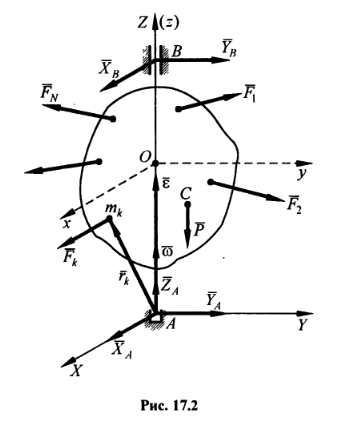
\includegraphics[scale = 0.5]{img/17.2.jpeg}
        \end{figure}
    
    \par Уравнения для определения реакций опор можно составить в проекциях  на  оси  как  неподвижной,  так  и  подвижной  системы  координат,  жестко связанной с вращающимся телом. 
    
    \par В первом случае при вращении тела будет изменяться распределение массы,  а значит, и моменты инерции тела относительно осей координат. Во втором случае моменты инерции тела относительно осей связанной с ним системы координат и координаты центра масс будут некоторыми постоянными величинами. Поэтому будем  полагать, что система координат $AXYZ$ жестко соединена с твердым телом
    
    \par За центр приведения сил инерции твердого тела примем точку $A$. Определим проекции на оси координат главного вектора и главного момента относительно точки $A$ сил инерции тела
    
    \par Главный вектор сил инерции
    
    \par $\vec{R} = -M \vec{a}_c = -M \vec{a}_c^{(n)} - M \vec{a}_c^{(\tau)}$
    
    \par Касательное $\vec{a}_c^{(\tau)}$ и нормальное  $\vec{a}_c^{(n)}$ ускорения центра масс тела соответственно равны
    
    \par $\vec{a}_c^{(\tau)} = \vec{\mathcal{E}} \times \vec{r}_c = 
    \begin{vmatrix}
      \vec{I}& \vec{J}& \vec{K}\\
      0& 0& \mathcal{E}_z\\
      X_c& Y_c& Z_c\\
    \end{vmatrix};$
    
    \quad 
    
    $\vec{a}_c^{(n)} = \vec{\omega} \times \vec{v}_c = 
    \begin{vmatrix}
      \vec{I}& \vec{J}& \vec{K}\\
      0& 0& \omega_z\\
      v_{cx}& v_{cy}& v_{zc}\\
    \end{vmatrix};$
    
    \par Раскрывая определители по элементам первой строки и принимая во внимание, что $\vec{v}_c = \vec{\omega} \times \vec{r}_c $, получаем
    
    \par  $\vec{a}_c^{(\tau)} = -\mathcal{E}_z{Y}_C\vec{I} + \mathcal{E}_z{X}_C\vec{J} + 0*\vec{K}; \quad \vec{a}_c^{(n)} = -\omega_z^2X_c\vec{I} - \omega_z^2Y_c\vec{J} + 0*\vec{K}.$
    
    \par Таким образом, для проекций главного вектора сил инерции тела на оси подвижной системы координат AXYZ имеем следующие выражения:
    \par
    $R_X^{\text{ин}}=M\mathcal{E}_zY_c + M\omega_z^2X_c; \quad R_Y^{\text{ин}}=-M\mathcal{E}_zX_c + M\omega_z^2Y_c ; \quad R_z^{\text{ин}}=0.$ \quad (17.13)
    
    \par Так как для определения реакций опор используется связанная с вращающимся телом система координат, то главный момент сил инерции относительно точки A можно представить в соответствии с формулой Бура в виде:
    \par               
    \par 
    $\Vec{L}_A^{\text{ин}} = -\frac{d\vec{K}_a}{dt}=-(\frac{\Vec{d}\vec{K}_a}{dt} + \Vec{\omega}\times \vec{K}_a)$ \qquad (17.14)
    
    \par Так как при вращении тела вокруг неподвижной оси $O_z\omega_X=\omega_Y=0 $, то главный момент количеств движения твердого тела относительно точки A определяется по формуле: 
    
    \par $\vec{K}_A=-J_{XZ}\omega_Z\vec{I} - J_{YZ}\omega_Z\vec{J} + J_Z\omega_Z\vec{K}$ \qquad (17.15)
    
    \par где $J_XZ= \sum\limits_{k=1}^Nm_kX_kZ_k, \quad J_YZ= \sum\limits_{k=1}^Nm_kY_kZ_k$ -центробежные моменты инерции тела;
    
    \par $J_Z= \sum\limits_{k=1}^Nm_k(X_k^2+Y_k^2)$ — момент инерции тела относительно оси OZ.
    
    \par Принимая во внимание (17.15) и учитывая, что $\Vec{\omega}\times\Vec{K}_A = J_{YZ}\omega_Z^2\vec{I} - J_{XZ}\omega_Z^2\vec{J} $ 
    
    \par из  (17.14) получим следующие  выражения  для  проекций  главного  момента сил инерции тела относительно точки A на оси системы координат AXYZ:
    
    \par ${L_X}^{\text{ин}}=J_XZ\mathcal{E}_Z-J_YZ\omega_Z^2; \quad L_Y^{\text{ин}}=J_YZ\mathcal{E}_Z+J_XZ\omega_Z^2
    ; \quad L_Z^{\text{ин}}=-J_Z\mathcal{E}_Z $ \quad (17.16)
    
    \par В соответствии с методом кинетостатики приравняем к нулю проекции на оси координат главного вектора и главного момента относительно точки A активных сил $\vec{F}_k $, реакций связей ($\vec{R}_A, \vec{R}_B $) и сил инерции точек тела. Учитывая полученные выше выражения (17.13) и (17.16), запишем:

    \par $X_A + X_B + \sum\limits_{k=1}^NF_{kX}+M\mathcal{E}_ZY_C+M\omega_Z^2X_C=0$; \qquad (17.17)

    \par $Y_A + Y_B + \sum\limits_{k=1}^NF_{kY}-M\mathcal{E}_ZX_C+M\omega_Z^2Y_C=0$; \qquad (17.18)

    \par $Z_A + \sum\limits_{k=1}^NF_{kZ}=0$; \qquad (17.19)

    \par $-Y_BAB+ \sum\limits_{k=1}^N M_X(\Vec{F}_k)+ J_{XZ}\mathcal{E}_Z-J_{YZ}\omega_Z^2=0$; \qquad (17.20)

    \par $X_BAB+ \sum\limits_{k=1}^N M_Y(\Vec{F}_k)+ J_{YZ}\mathcal{E}_Z-J_{XZ}\omega_Z^2=0$; \qquad (17.21)
    
    \par $\sum\limits_{k=1}^N M_Z(\Vec{F}_k)- J_{Z}\mathcal{E}_Z=0$; \qquad (17.22)

    \par Уравнение  (17.22)  не  содержит  реакций  опор.  При  известном  моменте инерции $J_Z$  и  заданных  внешних  силах  оно  позволяет  определить  угловое ускорение $\mathcal{E}_Z$(t) и угловую скорость  $\omega_Z=\int \mathcal{E}_Z dt+C_1$ твердого тела.Уравнения  (17.17)  –  (17.21)  дают возможность вычислить  проекции  на оси координат реакций подшипника  ($X_B , Y_B $) и подпятника  ($X_A,Y_A,Z_A $) В них входят слагаемые, зависящие как от заданных сил $\Vec{F}_k $, так и от сил инер-ции,  обусловленных  вращением  тела  с  угловой  скоростью $\omega_Z$  и  угловым ускорением $\mathcal{E}_Z$. Так как эти уравнения линейны, то каждую из реакций опор можно разделить на две составляющие,  называемые условно статической и динамической.Статические реакции опор вызываются только внешними силами; силы инерции при определении статических реакций полагают равными нулю. В этом случае

    \par $ X_B^{\text{ст}}=-\frac{1}{AB} \sum\limits_{k=1}^N M_Y(\Vec{F}_k); \quad Y_B^{\text{ст}}=\frac{1}{AB} \sum\limits_{k=1}^N M_X(\Vec{F}_k) $

    \par  $ X_A^{\text{ст}}=\frac{1}{AB} \sum\limits_{k=1}^N M_Y(\Vec{F}_k)- \sum\limits_{k=1}^NF_{kX}; \quad Y_A^{\text{ст}}=\frac{1}{AB} \sum\limits_{k=1}^N M_X(\Vec{F}_k) - \sum\limits_{k=1}^NF_{kY} $

    \par $Z_A^{\text{ст}}=- \sum\limits_{k=1}^NF_{kZ}$

    \par Динамические реакции опор зависят только от сил инерции. Уравнения для определения проекций динамических реакций подшипника и подпятника имеют вид

    \par $X_A^{\text{д}}+X_B^{\text{д}} + M \mathcal{E}_Z Y_C + M\omega_Z^2X_C=0$ \qquad (17.23)

    \par $Y_A^{\text{д}}+Y_B^{\text{д}} + M \mathcal{E}_Z X_C + M\omega_Z^2Y_C=0$ \qquad (17.24)

    \par $ -Y_B^{\text{д}}AB + J_{XZ}\mathcal{E}_Z - J_{YZ}\omega_Z^2=0$ \qquad (17.25)

    \par $ X_B^{\text{д}}AB + J_{YZ}\mathcal{E}_Z - J_{XZ}\omega_Z^2=0$ \qquad (17.26)

    \par Определив из уравнений (17.26) и (17.25) $X_B^{\text{д}} = - \frac{1}{AB} (J_{YZ}\mathcal{E}_Z + J_{XZ}\omega_Z^2); \quad  X_B^{\text{д}} = \frac{1}{AB}(J_{XZ}\mathcal{E}_Z - J_{YZ}\omega_Z^2)$
    
    \par  $$ \text{получаем:  }R_B^{\text{д}} = \frac{1}{AB} \sqrt{(\varepsilon_Z^2 + \omega_Z^4)(J_{XZ}^2 + J_{YZ}^2)}$$

    \par $$\text{Аналогично находим} R_A^{\text{д}} = \frac{1}{AB} (\{\mathcal{E}_Z^2 + \omega_Z^4\} \times ((J_{XZ}^2 + J_{YZ}^2)+M^2(X_C^2+Y_C^2)AB^2-2M(J_{XZ}X_C+J_{YZ}Y_C)AB))^{1/2}   $$

    \par Как видно, динамические реакции подшипника и подпятника зависят от угловой скорости и углового ускорения тела, а также от распределения массы тела относительно оси его вращения.

 
\end{center}
%30
\section{Понятие статической и динамической уравновешенности твердого тела, вращающегося вокруг неподвижной оси.}
\begin{center}
    \par\textbf{Статическая уравновешенность}

	  \par Твердое тело, вращающееся вокруг неподвижной оси, называют \textbf{статически уравновешенным}, если ось вращения проходит через его центр масс. В этом случае главный вектор сил инерции равен нулю, и из уравнений (17.23) и (17.24) получаем $ X_B^D = -X_A^D, \quad Y_B^D = -Y_A^D$. Это значит, что $ \vec R_B^D = -\vec R_A^D$, т.е. динамические реакции подшипника и подпятника образуют пару. Модули сил этой пары в соответствии с (17.27) и (17.28) определяются выражением

	  $$ R_A^D = R_B^D = \frac{1}{AB} \sqrt{(\varepsilon_Z^2 + \omega_Z^4)(J_{XZ}^2 + J_{YZ}^2)}.$$

	  \par Полученный результат не зависит от выбора центра приведения системы сил. Действительно, если в качестве центра приведения выбрать произвольную точку O на оси вращения тела (см. рис. 17.2), то уравнение (17.26) будет иметь следующий вид:

	  $$ \sum\limits_{k=1}^N M_y (\vec F_k) = - X_A^D OA + X_B^D OB + J_{yz} \varepsilon_Z + J_xz \omega_Z^2 = 0.$$
	  
	 \par Так как ось вращения тела - центральная, то $X_A^D = -X_B^D$ и тогда

	 $$X_B^D = -\frac{1}{AB} (J_{xz} \omega_z^2 +J_{yz} \varepsilon_z),$$
	 
	 \par что аналогично выражению для $X_B^D$ в случае, когда за центр приведения си-стемы сил была принята точка A. Такой же результат получается для $Y_A^D$ и $Y_B^D$. Не меняются при изменении центра приведения и центробежные моменты инерции тела, т.е. $J_{XZ} = J_{xz}$ и $J_{YZ} = J_{yz}$. Например:

	 $$ J_{XZ} = \sum\limits_{k=1}^N m_k x_k z_k = \sum\limits_{k=1}^N m_k X_k (Z_k - OA) = \sum\limits_{k=1}^N m_k X_k Z_k - OA\sum\limits_{k=1}^N m_k X_k.$$

	 \par Так как $\sum\limits_{k=1}^N m_k X_k Z_k == J_{XZ}.$

	 \par Таким образом, в случае статической уравновешенности тела динамические реакции опор приводятся к паре сил и могут быть не равны нулю. Пара сил инерции может быть уравновешена только парой — динамическими реакциями опор. Модули реакции зависят от угловой скорости $\omega_Z$ и углового ускорения $\varepsilon_Z$ твердого тела, распределения массы по его объему (что характеризуется центробежными моментами инерции $J_{XZ}$ и $J_{YZ}$), а также от расстояния между опорами.

	 \par\textbf{Динамическая уравновешенность}

	 \par Твердое тело, вращающееся вокруг неподвижной оси, называют \textbf{динами-чески уравновешенным},если равны нулю динамические реакции подшипника и подпятника. Из уравнения (17.27) следует, что динамическая реакция $\vec R_B^D$ подшипника будет равна нулю, если $J_{XZ} = J_{YZ} = 0$, т.е. если ось AZ вращения тела будет его главной осью инерции в точке A. Чтобы при этом была равна нулю и динамическая реакция подпятника, необходимо, как это следует из (17.28),  чтобы равнялись нулю  не  только  центробежные  моменты  инерции $J_{XZ}$ и $J_{YZ}$, но и координаты $X_C$ и $Y_C$ центра масс тела. Второе условие может быть выполнено, если ось AZ будет проходить через центр масс тела, т. е. будет центральной  осью. Таким  образом,  вращающееся  вокруг  неподвижной оси твердое тело будет динамически уравновешено, если ось вращения является его главной центральной осью инерции.
	 \par В случае, когда ось OZ вращения тела является его главной осью инерции в какой-либо точке O (см. рис. 17.2), но не проходит через центр масс, центробежные моменты инерции $J_{XZ} = 0, \quad J_{YZ} = 0$ и уравнения для определения динамических реакций подпятника А и подшипника B принимают вид

	 \par$ X_A^D + X_B^D + M \varepsilon_Z Y_C + M \omega_Z^2 X_C = 0; \qquad (17.34)$
	 \par$ Y_A^D + Y_B^D - M \varepsilon_Z X_C + M \omega_Z^2 Y_C = 0; \qquad (17.35)$
	 \par$ Y_A^D OA - Y_B^D OB = 0; \qquad (17.36)$
	 \par$ -X_A^D OA + X_B^D OB = 0. \qquad (17.37)$

	 \par Отсюда находим

	 \par $R_A^D = M \frac{OB}{AB} \sqrt{(\varepsilon_Z^2 + \omega_Z^4)(X_C^2 + Y_C^2)}; \qquad$ (17.38)
  
	 \par $R_B^D = M \frac{OA}{AB} \sqrt{(\varepsilon_Z^2 + \omega_Z^4)(X_C^2 + Y_C^2)}. \qquad$ (17.39)

	 \par В этом случае главный момент сил инерции тела относительно точки O равен нулю, и система сил инерции приводится к равнодействующей, приложенной в точке O и равной по модулю $M \sqrt{(\varepsilon_Z^2 + \omega_Z^4)(X_C^2 + Y_C^2)}$. Поэтому динамическими реакциями опор будут параллельные силы $\vec R_A^D$ и $\vec R_B^D$, которые направлены противоположно равнодействующей сил инерции тела, а их модули (17.38), (17.39) обратно пропорциональны расстояниям от центра приведения O до соответствующей опоры.
	 
	 \par На основании вышеизложенного, можно сделать следующие выводы.1. Динамические реакции могут существовать даже тогда, когда ось вращения тела проходит через его центр масс. Динамические реакции опор образуют пару сил, модули которых зависят от центробежных моментов инерции тела, угловой скорости и углового ускорения.2.  Если  ось  вращения  тела  является  его  главной  и  центральной  осью инерции, то динамические реакции подшипника и подпятника равны нулю, а статические реакции зависят только от внешних сил.
\end{center}
%31
\section{Динамические уравнения Эйлера.}
\begin{center}
    \par Дифференциальные уравнения сферического движения  твердого тела
    \par Влияние внешних сил на кинематические характеристики сферического движения твердого тела вокруг точки O, неподвижной в инерциальной системе отсчета, изучим с помощью  теорем об изменении главного момента количеств движения и кинетической энергии для системы материальных точек (см. 15.5, 15.6):
    \par $ \vec{\dot{K}}_O = \vec{\dot{L}}_O$, $\dot{T} = W^{(e,i)} $,
    \par поскольку они позволяют исключить из уравнений динамики  силы, сходящиеся в точке О.
    \par Помимо инерциальной системы отсчета S0 с осями Оx, Оy, Оz и ортами $ \vec{i}, \vec{j}, \vec{k} $, введем жестко связанную с твердым телом вспомогательную систему координат S с началом в точке О, осями ОX, ОY, OZ и ортами $ \vec{I}, \vec{J}, \vec{K} $ .  Угловая скорость системы S относительно системы S0 тождественно  равна угловой скорости самого тела $\omega$. Система S удобна тем, что в ней постоянны три осевых $J_x,J_y,J_z $, и три центробежных $J_{xy}, J_{xz}, J_{yz} $,момента инерции тела.
    \par Направим оси системы S не произвольно, а так, чтобы они совпадали с главными осями инерции твердого тела в точке О. В таких осях для твердого тела упрощается расчет проекций его главного момента количеств движения относительно точки О и его кинетической энергии:
    \par $K_x = A \omega_X $ ; $K_y = B \omega_y $; $K_z = C \omega_z \qquad$ (16.9), 
    \par $ T = 0.5 K_0 \omega \cos{\alpha}= 0.5 (\omega_x K_x + \omega_y K_y + \omega_z K_z) \qquad$ (16.10)
    \par Здесь и далее буквами A, B, C обозначены соответствующие осевые моменты инерции тела относительно трех ортогональных главных осей инерции. При   А = В эллипсоид инерции тела в точке O имеет форму поверхности вращения вокруг оси ОZ, которую в этом случае называют осью динамической симметрии твердого тела, а само тело — динамически симметричным. На практике для выполнения равенства А = В телу из однородного материала придают форму тела вращения.
    \par Согласно (16.9), (16.10), вектор $\vec{K_0}$ образует острый угол $\alpha$ с вектором $\vec{\omega}$.  При этом $\vec{K_0}$ параллелен главной оси инерции тела, если $\vec{\omega}$ направлен по этой оси  инерции тела, и  $\vec{K_0}$ перпендикулярен  главной оси  инерции тела, если ей перпендикулярен $\vec{\omega}$.
    \par В соответствии с формулой Бура, запись вектора  $\vec{K_0}$ твердого тела в проекциях на оси системы S (см. (16.9)) влечет за собой необходимость применения теоремы о его изменении в специальном виде
    \par $\frac{ d\vec{K_0}}{dt} + \omega \times \vec{K_0} = \vec{L_0}$,
    \par предполагающем последующее проецирование именно на оси системы S:
    \par $A \dot{\omega}_x + (C-B) \omega_y \omega_z = L_x$
    \par $B \dot{\omega}_y + (A-C) \omega_z \omega_x = L_y \qquad $ (16.11)
    \par $C \dot{\omega}_z + (B-A) \omega_x \omega_y = L_z$
    \par Систему уравнений (16.11) называют динамическими уравнениями Эйлера. Они устанавливают связь между моментами внешних сил и проекциями угловой скорости $\vec{\omega}$ тела. Каждое уравнение системы (16.11) содержит произведение проекций вектора $\vec{\omega}$, поэтому динамические уравнения Эйлера являются нелинейными дифференциальными уравнениями относительно этих проекций.
    \par Но поскольку расчет проекций вектора $\vec{\omega}$  на подвижные оси системы S не является конечной целью анализа, ибо остается нерешенной задача о пространственной ориентации этих осей, то динамические уравнения Эйлера дополняют кинематическими уравнениями  Эйлера  (4.8)
    \par 
\end{center}
%32
\section{Приближенная теория гироскопа. Основные понятия и допущения.}
\begin{center}
    \par Приближенная теория гироскопа построена на теореме об изменении вектора $\vec{K}_{O}$ в форме:

    \par $   \vec{K_{O}} = \vec{\Omega}_{K} \times \vec{K}_{O} = \vec{L}_{0} $

    \par Здесь приближенно считают, что неподвижный относительно твердого тела постоянный  по  модулю  вектор $\vec{K}_{0} $  вращается  относительно  системы $S_{0}$  с угловой скоростью $\Vec{\Omega}_{K}$.

    \par \textbf{Допущения}

    \par 1. Модуль проекции вектора $\vec{\omega}$ на главную ось инерции $OZ$ тела много больше модулей остальных проекций:

    \par $\omega^{2}_{Z} >> \omega^{2}_{X} + \omega^{2}_{Y} $ \qquad  (16.47)
    \par Из кинематических уравнений Эйлера в этом случае следует
    \par $ \dot \varphi^{2} >> \dot \Psi^{2} + \dot \theta^{2}$

    \par 2. Проекция вектора $\vec{\omega}$  на главную ось инерции OZ тела  постоянна по модулю:

    \par $\omega_{z} = const = \omega_{C} >0 $ \qquad  (16.49)
    \par 3. Модуль проекции вектора $ \vec{K}_{0}$ на OZ много больше остальных проекций (рис. 16.13):
    \par $K_{Z}^{2} >> K_{X}^{2} + K_{Y}^{2} $ \qquad  (16.50)
    \par или $(C\omega_{Z})^{2} >> (A\omega_{X})^{2} + (B\omega_{Y})^{2} $

    \begin{figure}[H]
    \centering 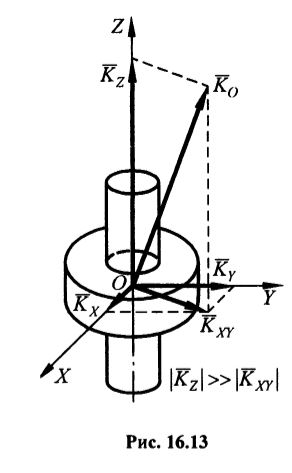
\includegraphics[scale = 0.5]{img/16.13.JPG}
    \end{figure}

    \par Для тел с соотношением главных моментов инерции С>A, C>B условие (16.50) является следствием (16.47).

    \par 4. Вектор  $K_{0}^{2}$  имеет  постоянный  модуль,  равный его проекции на ось собственного вращения OZ:

    \par $K_{0} = \sqrt{(A\omega_{X})^{2} + (B\omega_{Y})^{2} + (C\omega_{Z})^{2}}  =C\omega_{Z} = C\omega_{C} =K_{Z} = const $ \qquad  (16.51)

    \par 5. Вектор  $\vec{K}_{0}$ направлен по оси OZ тела:
    \par $\vec{K}_{0} = A\omega_{X}\vec{I} + B\omega_{Y}\vec{J} + C\omega_{Z}\vec{K} = C\omega_{Z}\vec{K} = C\omega_{C}\vec{K} $ \qquad  (16.52)

    \par 6. Вектор главного момента внешних сил $\vec{L}_{0}$ перпендикулярен к вектору $\vec{K}_{0}$. Неперпендикулярность  $\vec{L}_{0}$ и  $\vec{K}_{0}$ приводит к изменению модуля  $\vec{K}_{0}$, что противоречит четвертому допущению. 
    
\end{center}
%33
\section{Особенности движения оси гироскопа. Теорема Резаля. Правило прецессии.}
\begin{center}
    \par \textbf{Особенности движения оси гироскопа}
    \par \underline{1)Покоится}
    \begin{figure}[H]
        \centering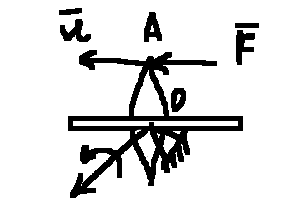
\includegraphics[scale=0.5]{img/1.jpeg} 
    \end{figure}
    \par Если тело испытывает силу, приложенную к т.А, то тело будет вращаться вокруг оси Ох. т. А двигаться в направлении действия силы. По завершению действия силы, тело по инерции продолжит вращаться вокруг оси Ох

    \par \underline{2)Вращается}
    \begin{figure}[H]
        \centering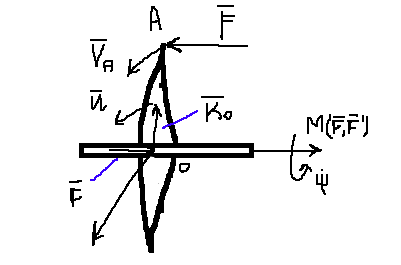
\includegraphics[scale=0.5]{img/2.jpeg} 
    \end{figure}
    \par Приложенная к т.А сила F создает момент этой силы относительно точки О и в соответствии с теоремой Резаля точка А начнет перемещаться с прецессирующей осью вокруг оси Оу. По завершении действия силы, прецессия прекратится, а это значит, что прецессия не имеет инерции
        $$\dot \psi = \frac{u}{|\vec K_0|} = \frac{u}{OB}$$
        $$\psi = \frac{u}{OB} \tau = \frac{L^e}{K_0} \tau$$
        
        \par $\vec{L}_0=\vec{\omega}_2\times \vec{K}_0$

        \par $L_0=\left| \vec{\omega}_2\times J_z\vec{\omega}_1\right|=J_z\left| \vec{\omega}_2\times \vec{\omega}_1  \right|=J_z\omega_{1} \omega_{2} sin\theta$
    \par При ударе ось гироскопа практически не отклоняется от своего положения.

    \par \textbf{Теорема Резаля:} 
    
    \par при движении механической системы скорость точки, совпадающей с концами вектора кинетического момента при движении по годографу равна по величине и направлению главному моменту всех внешних сил системы

    \par $\vec{L}_0^{e}=\vec{U}$

    \par \textbf{Правило прeцессии:}

    \par Если к вращающемуся вокруг собственной оси гироскопу приложить внешние силы, создающие момент относительно неподвижной точки, то та часть оси гироскопа по которой направлен кинетический момент $\vec{K}_0$, начнет прецессировать в направлении момента внешних сил $\vec{L}_0^{(e)}$ 
    
\end{center}
%34
\section{Гироскопический момент. Правило Жуковского.}
\begin{center}
    \par \textbf{Гироскопический момент.}
    
    \par При изучении свойств прецессии было установлено, что главная ось гироскопа движется не в направлении приложенной силы, а перпендикулярно направлению действующей силы. Такое явление может произойти только в том случае, если со стороны гироскопа возникает сила реакции, уравновешивающая приложенную к гироскопу внешнюю силу. Эта сила противодействия, препятствующая движению гироскопа по направлению действия силы, называется гироскопической реакцией, а ее момент, уравновешивающий момент внешних сил $\vec{L}$, — моментом гироскопической реакции, или гироскопическим моментом.
    
    \par \textbf{Правило Жуковского:}
    
    \par Направление угловой скорости прецессии совпадает с направлением кратчайшего поворота $\vec{K}_0$ к  $\vec{L}_0$       
    
    \begin{figure}[H]
        \centering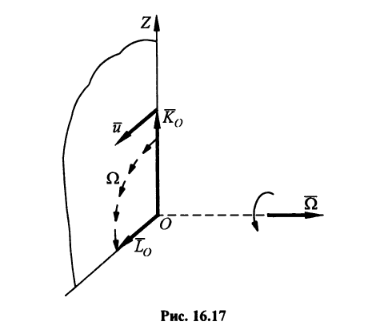
\includegraphics[scale=0.5]{img/16.17.jpeg} 
    \end{figure}

\end{center}
%35
\section{Основные положения теории удара.}

\begin{center}
В излагаемой ниже теории удара рассматривают такие ударные явления, при которых происходит конечное изменение скоростей точек механической системы за весьма малый промежуток времени τ, называемый временем удара.

Запишем дифференциальное уравнение  движения  материальной точки массой m в виде:

$ d(m\vec{V}) = \vec{F}dt = d\vec{S}$   

\par и проинтегрируем его в пределах от 0 до $\tau$

\par $ m(\vec{u}-\vec{v}) = \int\limits_0^\tau \vec{F}dt = \vec{S}   \qquad \qquad (20.2) $ 

\par  Здесь $\vec{V}$  — скорость точки в процессе удара; $\vec{v} \vec{u}$, — скорости точки до и после удара соответственно; $\vec{S}$  — импульс ударной силы $\vec{F}$ за время $\tau$.

\par Изменение скорости точки $∆\vec{v} = \vec{u} - \vec{v}$ за время удара есть величина конечная, что следует из эксперимента. Из предыдущего выражения следует, что им-пульс ударной силы также величина конечная.Запишем импульс ударной силы с помощью теоремы о среднем значении функции:

\par $\vec{S} = \int\limits_0^\tau \vec{F}dt = \vec{F}_{cp} \tau \qquad \qquad (20.3) $

\par где $\vec{F}_{cp}$ — среднее значение ударной силы за время удара.

\par из последних двух выражений получаем:

\par $\vec{F}_{cp}=\frac{m(\vec{u}-\vec{v})}{\tau}$

\par т. е. при конечном значении произведения в числителе и очень малом знаменателе ($\tau \approx 10^{-2} - 10^{-4} c$)   $\vec{F}_{cp}$ очень велико (порядка $\frac{1}{\tau}$). В связи с этим при $\tau$→0 и  $\vec{F}_{cp}$→∞ импульс $\vec{S}$ есть величина конечная.

\par Согласно принятому допущению, в уравнениях теории удара время отсутствует, поэтому вместо ударных сил будем оперировать их импульсами.

\par Уравнение (20.2) выражает теорему об изменении количества движения точки при ударе. Покажем, что перемещение $∆\vec{r}$ точки за время удара бесконечно мало. Интегрируя уравнение

\par $m\frac{d\vec{r}}{dt}=\vec{S}+m\vec{v}$

\par от 0 до $\tau$, получаем

\par $\vec{r}-\vec{r}_0 = ∆\vec{r} = (\vec{v} + \frac{\vec{S}_{cp}}{m})\tau \qquad \qquad (20.4) $

\par Здесь $\vec{S}_{cp} = \int\limits_0^\tau \frac{\vec{S}dt}{\tau}$ — средний ударный импульс силы;
      $\vec{S}_{cp} = \int\limits_0^t \vec{F}dt$ при $0 < t \leqslant \tau$

\par При конечных $\vec{v},  \vec{S}_{cp}$ и $\tau$→0  перемещение точки $∆\vec{r}$ за время удара пренебрежимо мало и его при ударе не учитывают

\par Пусть на точку действуют ударная сила $\vec{F}(t)$ и конечная сила $\vec{P}$. В качестве конечных можно рассматривать силы тяжести, упругости, а также силы, зависящие, например, от скорости точки. Суммарный импульс этих сил равен

\par $\vec{S}_\Sigma = \int\limits_0^\tau \vec{F}dt + \int\limits_0^\tau \vec{P}dt = 
\vec{S} + \vec{P}_{cp}\tau$

\par Вторым слагаемым здесь можно пренебречь, так как оно является малым того же порядка, что и $\tau$, а $\vec{S}$  — величина конечная, поэтому при ударе действие конечных сил не учитывается.

\par Используя модель Ньютона, рассмотрим удар двух тел, при котором в точке контакта A возникают ударные силы. Трение не будем учитывать, поэтому ударные силы и их импульсы $\vec{S}$  и $\vec{S}'$  направлены по общей нормали к соударяющимся телам в точке A (рис. 20.1)

\par Ударная сила, действующая на тело, изменяется во времени, как показано на рис. 20.2.

%рисунок 20.1 и 20.2%
\begin{figure}[H]
    \centering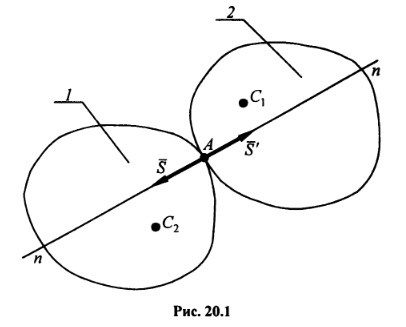
\includegraphics[scale=0.5]{img/20.1.jpeg} 
    \qquad \qquad
    \centering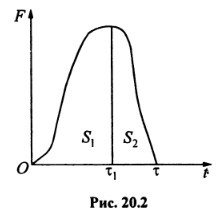
\includegraphics[scale=0.6]{img/20.2.jpeg}
\end{figure}

\par В контакте тел образуются местные упругопластические деформации, зависящие от физических свойств тел. Процесс удара разбивается на две фазы. В первой фазе — фазе деформирования — происходит сближение тел в точке A по общей нормали до тех пор, пока нормальная составляющая относительной скорости точки контакта тел не обратится в нуль в момент времени $\tau_1$. Фаза деформирования характеризуется импульсом ударной силы $S_1$. Далее начинается вторая фаза — фаза восстановления, при которой тела в месте контакта восстанавливают свою форму вследствие упругих сил. Нормальная составляющая относительной скорости точки контакта меняет знак и возрастает, но из-за пластических деформаций не достигает своего первоначального значения. Импульс ударной силы в этой фазе равен $S_2$

\par Введем коэффициент восстановления K, который характеризует свойства материалов соударяющихся тел:

\par $K = \frac{S_2}{S_1} =\frac{S_2'}{S_1'}$ \qquad \qquad (20.5),

\par где $S_1$, $S_1'$, $S_2$, $S_2'$ — импульсы ударных сил в фазах деформирования и восстановления для первого и второго тел соответственно.

\par Коэффициент  восстановления определяют  экспериментально.  Так  как после удара в общем случае полного восстановления формы тел не происходит, то $0\leqslant K \leqslant 1$ . При K = 1 удар называют \textbf{абсолютно упругим}, при  K=0  — \textbf{абсолютно неупругим}, а при $0<K<1$  — \textbf{упругим}. В случае, когда  K=0 , нормальная составляющая относительной скорости точки соприкосновения тел после удара равна нулю и фаза восстановления отсутствует. Оба тела либо движутся совместно, либо одно тело скользит по другому после максимального сближения в точке контакта

\end{center}

%36
\section{Теорема об изменении количества движения точки и системы точек при ударе.}

\begin{center}

\par Для материальной точки теорема об изменении количества движения при ударе имеет вид (20.2), т. е. изменение количества движения точки за время удара равно импульсу ударной силы, действующей на точку.

\par В  проекциях на  оси  прямоугольной  декартовой  системы  координат получаем

\par $mu_x - mv_x = S_x; \quad mu_y - mv_y = S_y; \quad mu_z - mv_z = S_z; $

\par Для ударных внутренних сил механической системы имеем

\par $\sum\limits_{k=1}^N \vec{F}_k^{(i)} = 0;
\quad \sum\limits_{k=1}^N \vec{M}_0\vec{F}_k^{(i)} = 0.$

\par Проинтегрировав по времени удара, получаем

\par $\sum\limits_{k=1}^N \vec{S}_k^{(i)} = 0;
\quad \sum\limits_{k=1}^N \vec{M}_0\vec{S}_k^{(i)} = 0. \quad\quad (20.6)$

\par Рассмотрим  механическую  систему,  состоящую  из  N  материальных  точек. Применим теорему  об  изменении количества  движения  для k-й точки системы:

\par $m_k \vec{u}_k - m_k \vec{v}_k = 
\vec{S}_k^{(e)} + \vec{S}_k^{(i)}, k = 1, \dots, N. \quad\quad (20.7)$

\par Здесь $\vec{u}_k, \vec{v}_k$,  — скорости  k-й точки  после и  до удара; $\vec{S}_k^{(e)}, \vec{S}_k^{(i)}$  — импульсы внешней и внутренней ударных сил.

\par Суммируя уравнения (20.7) по точкам системы, получаем

\par $\sum\limits_{k=1}^N m_k \vec{u}_k - \sum\limits_{k=1}^N m_k \vec{v}_k = \sum\limits_{k=1}^N m_k \vec{S}_k^{(e)} + \sum\limits_{k=1}^N m_k \vec{S}_k^{(i)}$

\par Обозначив $\vec{Q} = \sum\limits_{k=1}^N m_k \vec{u}_k, \quad \vec{Q}_0 = \sum\limits_{k=1}^N m_k \vec{v}_k$ с  учетом  свойства  (20.6)  из  (20.7) находим

\par $\vec{Q} - \vec{Q}_0 = \sum\limits_{k=1}^N \vec{S}_k^{(e)}, \quad\quad (20.8)$

\par где $\vec{Q}, \vec{Q}_0$ — количества движения системы после и до удара соответственно.

\par Таким образом, изменение количества движения механической системы за время удара  равно векторной  сумме импульсов  всех внешних  ударных сил,  действующих на точки системы.

\par В проекциях на оси прямоугольной декартовой системы координат имеем

\par ${Q}_x - {Q}_{0x} = \sum\limits_{k=1}^N \vec{S}_{kx}^{(e)}; \quad {Q}_y - {Q}_{0y} = \sum\limits_{k=1}^N \vec{S}_{ky}^{(e)}; \quad {Q}_z - {Q}_{0z} = \sum\limits_{k=1}^N \vec{S}_{kz}^{(e)}. \quad\quad (20.9)$

\par Запишем  $\vec{Q} = M \vec{u}_c, \vec{Q}_0 = M \vec{v}_c$, где $M, \vec{u}_c, \vec{v}_c$  — соответственно масса си-стемы и скорости ее центра масс после и до удара. Согласно (20.8), выражение для теоремы о движении центра масс системы имеет вид

\par $M \vec{u}_c - M \vec{v}_c = \sum\limits_{k=1}^N \vec{S}_k^{(e)}. \quad\quad  (20.10)$

\par В проекциях на оси координат получаем

\par $M (\vec{u}_{cx} - \vec{v}_{cx}) = \sum\limits_{k=1}^N \vec{S}_{kx}^{(e)}; M (\vec{u}_{cy} - \vec{v}_{cy}) = \sum\limits_{k=1}^N \vec{S}_{k_y}^{(e)}; M (\vec{u}_{cz} - \vec{v}_{cz}) = \sum\limits_{k=1}^N \vec{S}_{kz}^{(e)}. \quad\quad (20.11)$

\par Приведем законы сохранения, вытекающие из этих теорем

\par 1. Если $\sum\limits_{k=1}^N \vec{S}_k^{(e)} = 0$, то из (20.8), (20.10) следует 

\par $\vec{Q} = \vec{Q}_0, \quad \vec{u}_c = \vec{v}_c \quad\quad (20.12)$

\par Таким образом, если векторная сумма импульсов внешних ударных сил равна нулю, то вектор количества движения и скорость центра масс системы остаются постоянными. В проекциях на оси координат имеем

\par $Q_x=Q_{0x}; Q_y=Q_{0y}; Q_z=Q_{0z}$

\par $u_{cx}=v_{cx}; u_{cy}=v_{cy}; u_{cz}=v_{cz}$

\par 2. Если $\sum\limits_{k=1}^N \vec{S}_{kx}^{(e)} = 0$, то из (20.9), (20.11) получаем

\par $Q_x=Q_{0x}, u_{cx}=v_{cx}.$

\end{center}
%37
\section{Теорема об изменении кинетического момента точки и механической системы при ударе.}
\begin{center}

\par $ m(\vec{u}-\vec{v}) = \int\limits_0^\tau \vec{F}dt = \vec{S}   \qquad \qquad (20.2) $ 

\par Умножим векторно равенство (20.2) слева на радиус-вектор $\vec{r}$ (рис. 20.4)

%рисунок 20.4%
\begin{figure}[H]
    \centering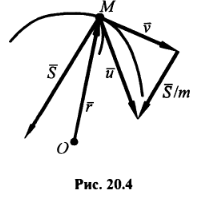
\includegraphics[scale=0.5]{img/20.4.jpeg} 
\end{figure}

\par $\vec{r} \times m \vec{u} - \vec{r} \times m \vec{v} = \vec{r} \times \vec{S},$ или $\vec{M}_0(m \vec{u}) - \vec{M}_0(m \vec{v}) = \vec{M}_0 (\vec{S}) \quad\quad (20.13)$

\par где $\vec{M}_0(m \vec{u}), \vec{M}_0(m \vec{v}), \vec{M}_0(\vec{S})$  —  моменты  количества  движения  материальной точки после и до удара и момент импульса ударной силы относительно точки O соответственно.

\par Уравнение (20.13) выражает теорему об изменении момента количества движения материальной точки относительно точки O при ударе

\par В проекциях на оси прямоугольной декартовой системы координат получаем

\par $\vec{M}_x(m \vec{u}) - \vec{M}_x(m \vec{v}) = \vec{M}_x (\vec{S}) ;$

\par $\vec{M}_y(m \vec{u}) - \vec{M}_y(m \vec{v}) = \vec{M}_y (\vec{S}) ;$

\par $\vec{M}_z(m \vec{u}) - \vec{M}_z(m \vec{v}) = \vec{M}_z (\vec{S}) ;$

\par Запишем  уравнение,  выражающее  теорему  об изменении момента количества  движения для любой из N точек механической системы

\par $\vec{r}_k \times m \vec{u}_k - \vec{r}_k \times m \vec{v}_k = \vec{r}_k \times \vec{S}_k^{(e)} + \vec{r}_k \times \vec{S}_k^{(i)}, k=1, \dots, N, \quad\quad\quad (20.14) $

\par где $\vec{u}_k, \vec{v}_k$  — скорости k-й точки после и до удара; $\vec{S}_k^{(e)}, \vec{S}_k^{(i)}$,  — импульсы внеш-ней и внутренней ударных сил, действующих на k-ю точку системы.

\par Суммируя (20.14) по всем точкам системы, получаем

\par $\vec{K}_0 - \vec{k}_0^{(0)} = \sum\limits_{k=1}^N \vec{M}_0 (\vec{S}_k^{(e)}), \quad\quad\quad (20.15)$

\par где $\vec{K}_0 = \sum\limits_{k=1}^N \vec{r}_k \times m_k \vec{u}_k, \vec{K}_0^{(0)} = \sum\limits_{k=1}^N \vec{r}_k \times m_k \vec{v}_k$ — главные моменты количеств движения системы  относительно  точки  O  после  и  до  удара, $\sum\limits_{k=1}^N \vec{M}_0 (\vec{S}_k^{(e)}) = \sum\limits_{k=1}^N \vec{r}_k \times (\vec{S}_k^{(e)})$ —  сумма  моментов  импульсов  внешних  ударных  сил  относительно  точки  O  ( $\sum\limits_{k=1}^N \vec{M}_0 (\vec{S}_k^{(e)}) = \sum\limits_{k=1}^N \vec{r}_k \times (\vec{S}_k^{(e)})$ по свойству внутренних сил).

\par Сформулируем теорему: \textbf{изменение главного момента количеств движения системы относительно какой-либо точки за время удара равно векторной сумме моментов импульсов внешних ударных сил, приложенных к материальным точкам системы, относительно той же точки}.

\par Для главных моментов количеств движения системы относительно осей координат имеем

\par $K_x - K_x^{(0)} = \sum\limits_{k=1}^N \vec{M}_x (\vec{S}_k^{(e)}); K_y - K_y^{(0)} = \sum\limits_{k=1}^N \vec{M}_y (\vec{S}_k^{(e)}); \quad\quad\quad\quad (20.16)$ 

\par $K_z - K_z^{(0)} = \sum\limits_{k=1}^N \vec{M}_z (\vec{S}_k^{(e)})$

\end{center}
%38
\section{Изменение угловой скорости при ударе по вращающемуся телу.}
\begin{center}

\par Рассмотрим теперь, как изменяется угловая скорость вращающегося тела при ударе. Пусть твердое тело вращается вокруг неподвижной оси $Az$ с угловой скоростью $\vec{\omega}_0$ (рис. 20.5). К телу приложены импульсы $\vec{S}_k^{(e)} (k=1, \dots, N)$  .  Определим  изменение угловой скорости $\vec{\omega}$ тела после их приложения.

%рисунок 20.5
\begin{figure}[H]
    \centering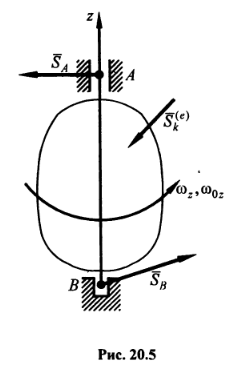
\includegraphics[scale=0.5]{img/20.5.jpeg} 
\end{figure}

\par Главные моменты  количеств движения тела относительно  оси  $Az$  после  и  до  удара  равны:$K_z = J_z \omega_z, K_z^{(0)} = J_z \omega_{0_z},$, где $Jz$ — момент инерции тела  относительно  оси  вращения.  Из  третьего уравнения (20.16) имеем

\par $J_z (\omega_z - \omega_{0_z}) = \sum\limits_{k=1}^N M_z (\vec{S}_k^{(e)}) \quad\quad\quad (20.17)$

\par откуда 

\par $∆\omega_z = \omega_z - \omega_{0_z} = \frac{\sum\limits_{k=1}^N M_z (\vec{S}_k^{(e)})}{J_z}$

\par где $∆\omega_z \omega_z$,  — изменение угловой скорости при ударе и проекция на ось $Az$ угловой скорости тела после удара (см. рис. 20.5). Моменты импульсов $\vec{S}_A, \vec{S}_B$,  ударных реакций относительно оси $Az$ при этом равны нулю.
    
\end{center}
%39
\section{Центр удара. Условия отсутствия ударных реакций в опорах вращающегося твердого тела}
\begin{center}

\par Пусть нам заранее известны следующие уравнения (без выводов) стр.531-532 учебника

\par $∆ \vec{Q} = \vec{Q} - \vec{Q}_0 = \vec{S} + \vec{S}_A + \vec{S}_B; \quad\quad\quad (20.32)$

\par $∆ \vec{K}_0 = \vec{K}_0 + \vec{K}_0^{(0)} = \vec{M}_0 (\vec{S}) + \vec{M}_0 (\vec{S}_A) + \vec{M}_0 (\vec{S}_B) \quad\quad\quad (20.33)$

\par $∆ \vec{Q} = m 
\begin{vmatrix}
  \vec{i}& \vec{j}& \vec{k}\\
   0& 0& ∆\omega \\
   x_c& y_c& z_c
\end{vmatrix}
=m[ \vec{i}(-y_c ∆\omega) + \vec{j}x_c ∆\omega + \vec{k}· 0 ] \quad\quad\quad (20.34)$

\par \quad

\par $K_x = -J_{xz} \omega_z, \quad K_y = -J_{yz} \omega_z, \quad K_z = -J_z \omega_z;$

\par \quad

\par $∆K_x = -J_{xz} ∆ \omega, \quad ∆K_y = -J_{yz} ∆ \omega, \quad ∆K_z = -J_z ∆ \omega, \quad\quad\quad (20.35) $

\par \quad

\par $∆ Q_x = -my_c ∆ \omega = S_x + S_{Ax} + S_{Bx}; ∆ Q_y = mx_c ∆ \omega = S_y + S_{Ay} + S_{By};$ 

\par $∆ Q_z = 0 = S_z + S_{Az}; ∆K_x = -J_{xz} ∆ \omega = M_x(\vec{S}) + M_x(\vec{S}_A) + M_x(\vec{S}_B); \quad\quad (20.36)$

\par $∆K_y = -J_{yz} ∆ \omega = M_y(\vec{S}) + M_y(\vec{S}_A) + M_y(\vec{S}_B); ∆K_z = J_{z} ∆ \omega = M_z(\vec{S})$

\par С помощью системы (20.36) при заданных импульсе $\vec{S}$  и точке его приложения определяют изменение угловой скорости $∆ \omega$ 

\par \textbf{Центр удара}

\par Рассмотрим теперь задачу о нахождении условий, при которых удар, произведенный по телу, не создает ударных реакций. Положим в (20.32), (20.33) $\vec{S}_A = \vec{S}_B = 0$ , тогда (20.36) принимает вид

\par $-my_c ∆ \omega = S_x; \quad -mx_c ∆ \omega = S_y; \quad 0 = S_z$

\par $-J_{xz} ∆ \omega = M_x (\vec{S}); -J_{yz} ∆ \omega = M_y (\vec{S}); -J_{z} ∆ \omega = M_z (\vec{S}); \quad\quad\quad (20.37)$

\par Из третьего  уравнения системы  (20.37) следует, что  импульс $\vec{S}$  должен быть  перпендикулярен  оси  вращения  тела  $Oz$.  Выберем  плоскость  $Oxy$  так, чтобы  в  ней  находился  импульс $\vec{S}$ ,  а  ось  $Ox$  направим  параллельно  $\vec{S}$  (рис. 20.12). Тогда $S_y = 0, S_x = S, M_x (\vec{S}) = M_y (\vec{S}) = 0$. Пусть $ON = l$. Уравнения (20.37) примут вид

\par $-my_c ∆ \omega = S; \quad -mx_c ∆ \omega = 0; \quad 0 = S_z$,

\par $-J_{xz} ∆ \omega = 0; \ -J_{yz} ∆ \omega = 0; \ J_{z} ∆ \omega = - l S$

%рис. 20.12%
\begin{figure}[H]
    \centering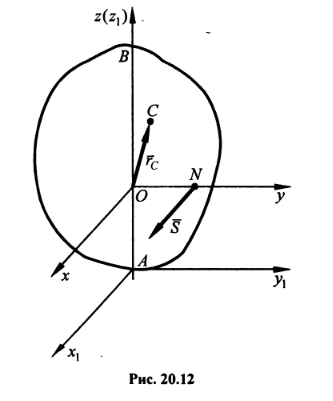
\includegraphics[scale=0.5]{img/20.12.jpeg} 
\end{figure}

\par Из второго уравнения имеем  $X_c = 0$, из четвертого  и  пятого  находим $J_{xz} = J_{yz} = 0$. Это означает, что центр масс тела лежит в плоскости $Oyz$, ось $Oz$ является главной для точки  O,  а  импульс $\vec{S}$ ударной  силы  перпендикулярен плоскости,  проходящей  через ось вращения и центр масс тела. Из первого и последнего уравнений получаем

\par $l = \frac{J_z}{(my_c)} \quad\quad\quad (20.38)$ 

\par Из (20.38) следует, что знаки $y_c$ и $l$ одинаковы, т. е. центр масс системы и точка N лежат в плоскости $Oyz$ по одну сторону от оси $Oz.$

\par \textit{Точка N, в которой приложен импульс $\vec{S}$ при отсутствии ударных реакций подшипников, называется} \textbf{центром удара}.

\par\fbox{\begin{minipage}{50em}
    Центром удара называется та точка твердого тела, вращающегося в закрепленной подпятником и подшипником \\\ оси, при котором ударные импульсы в опорных связях не возникают.
\end{minipage}}

\par Если центр масс системы находится на оси вращения, то $y_c=0$  и $l = ∞$, т. е. в этом случае центр  удара  отсутствует (из  уравнения (20.32)  следует $\vec{S}_A + \vec{S}_B = -\vec{S}$ ).  Отметим, что удары по уравновешенным вращающимся валам машин передаются на подшипники.

\par Итак, чтобы при приложении к телу, вращающемуся вокруг неподвижной оси, ударного импульса не возникали ударные реакции в опорах, т. е. чтобы существовал  центр  удара,  необходимо и  достаточно  выполнить  следующие условия:

\par\fbox{\begin{minipage}{50em}
    \par 1) ударный импульс должен быть перпендикулярен плоскости, проходящей через ось вращения тела и его центр масс;

    \par 2) точка N пересечения линии действия ударного импульса с плоскостью, проходящей через ось вращения тела и его центр масс, должна лежать в этой плоскости по одну сторону от оси вращения вместе с центром масс;

    \par 3) ударный импульс, произвольный по величине, должен лежать в плоскости, перпендикулярной  оси вращения и проходящей через  точку O, для которой ось вращения является главной осью инерции тела
\end{minipage}}
\end{center}
%40
\section{Теорема Карно.}
\begin{center}
    \par $\vec{V}$ - скорость до удара 
    \par $\vec{U}$ - скорость после удара 
    \par $\vec{S} = \vec{S}_1 + \vec{S}_2$, где $\vec{S}_1$ - фаза деформации, $\vec{S}_2$ - фаза восстановления
    \par (1) \underline{$m(\vec{U}-\vec{V})=\vec{S}$}
    \par (1)U\qquad $mU^{2} - m\vec{U}\vec{V}=\vec{S}\vec{U}$
    \par +
    \par (1)V\qquad $m\vec{U}\vec{V}-mV^{2}=\vec{S}\vec{V}$
    \par (2)\underline{$mU^{2}-mV^{2}=\vec{S}\vec{U}+\vec{S}\vec{V}$} => $mU^{2}-mV^{2}=\vec{S}(\vec{U}+\vec{V})$
    \par \textbf{(1) Фаза деформации.}
    \par при ударе тела деформируются и в момент, когда деформация максимальна, скорость:
    \par $\vec{V}$ - начальная скорость
    \par $\vec{U}_1 = \vec{U}_\tau \quad (\perp \vec{S}_1)$
    \par $mU_1^{2}-mV^{2}=\vec{S}_1(\vec{U}_1+\vec{V})$
    \par (*) $mU_1^{2}-mV^{2}=\vec{S}_1\vec{V}$
    \par Из (1):\quad $m(\vec{U}-\vec{V})=\vec{S}_1 \quad$ |*$\vec{S}_1$  
    \par $m\vec{U}_1\vec{S}_1-m\vec{V}\vec{S}_1=\vec{S}_1^{2}\quad => \vec{S}_1\vec{V}=-\frac{\vec{S}_1^{2}}{m}$
    \par Из (*) получаем: 
    \par (3)$m\vec{U}_1-m\vec{V}_1=-\frac{\vec{S}_1^{2}}{m}$
    \par \textbf{(2) Фаза восстановления.}
    \par $\vec{S}_2 || \vec{S}_1 \qquad \vec{S}_2\vec{U}_1=0$
    \par $\vec{U}_1$ - начальная скорость
    \par $\vec{U}$ - конечная скорость
    \par Из (2): $mU^{2}-mU_1^{2}=\vec{S}_2(\vec{U}+\vec{U}_1)$
    \par $mU^{2}-mU_1^{2}=\vec{S}_2\vec{U}$
    \par Из (1): $m(\vec{U}-\vec{U}_1)=\vec{S} \quad |*S_2$
    \par $m\vec{S}_2\vec{U}-m\vec{S}_2\vec{U}_1=S_2^{2}$
    \par $m\vec{S}_2\vec{U}=\vec{S}_2^{2}$
    \par $\vec{S}_2\vec{U}=\frac{S_2^{2}}{m}$
    \par $S=S_1+S_2; \quad S_2=kS_1; =>\quad S_1=\frac{S}{1+k}; \quad S_1-S_2=\frac{1-k}{1+k}S;$
    \par Тогда:
    \par (4)$mU^{2}-mU_1^{2}=\frac{S_2^{2}}{m}$
    \par Сложим (3) и (4) уравнения:
    \par $mU^{2}-mV^{2}=\frac{S_2^{2}}{m} - \frac{S_1^{2}}{m}$
    \par $mU^{2}-mV^{2}=-\frac{S_1^{2}-S_2^{2}}{m}$
    \par $mU^{2}-mV^{2}=-\frac{(S_1-S_2)(S_1+S_2)}{m}$
    \par $mU^{2}-mV^{2}=-\frac{S^{2}(1-k)}{(1+k)m}$
    \par $mU^{2}-mV^{2}=-\frac{S^{2}(1-k)}{(1+k)m} |*\frac{1}{2}$ \par $\frac{1}{2}mU^{2}-\frac{1}{2}mV^{2}=-\frac{1-k}{1+k} \frac{1}{2} \frac{S^{2}}{m}$
    \par $\frac{1}{2}mU^{2}-\frac{1}{2}mV^{2}=-\frac{1-k}{1+k} \frac{1}{2} m(\vec{U}-\vec{V})^{2}, $ 
    \par где $\quad m(\vec{U}-\vec{V})^{2}$ - кинетическая энергия точки с потерями скорости.
    \par $\frac{1}{2}m_{k}U_{k}^{2}-\frac{1}{2}m_{k}V_{k}^{2}=-\frac{1-k}{1+k} \frac{1}{2} m_{k}(\vec{U}_{k}-\vec{V}_{k})^{2}$ 
    \par $\sum\limits_{k=1}^N\frac{1}{2}mU^{2}-\sum\limits_{k=1}^N\frac{1}{2}mV^{2}=-\frac{1-k}{1+k}\sum\limits_{k=1}^N \frac{1}{2} m(\vec{U}-\vec{V})^{2}$ 
    \par\fbox{\begin{minipage}{10em}
        $T-T_0=-\frac{1-k}{1+k}T_\text{пот.}$
    \end{minipage}}  
    - Теорема Карно
    \par где T - кинетическая энергия до удара; $\quad T_0 -$ кинетическая энергия после удара; $\quad T_\text{пот.} -$ кинетическая энергия с потерями скорости (потерянная кинетическая энергия при ударе)
    \par\fbox{\begin{minipage}{30em}
        Потери кинетической энергии при ударе равны кинетической энергии системы, которая соответствует потерянным скоростям ее точек, умноженной на  $\frac{1-k}{1+k}$, k - коэффициент восстановления.
    \end{minipage}}  
\end{center}


%41
\section{Движение точки переменной массы. Дифференциальные уравнения движения.}
\begin{center}

\par Ограничимся рассмотрением тех случаев, для которых процесс изменения массы происходит непрерывно. При скачкообразном изменении массы соответствующие задачи решаются путем непосредственного применения общих теорем динамики тел постоянной массы, а также методами теории удара

\par Для вывода уравнения движения ТПМ воспользуемся теоремой об изменении количества движения механической системы.  Для этого рассмотрим механическую систему, состоящую из частиц постоянной массы, которые в момент времени t составляют материальную точку  \textbf{M} (обозначим массу точки $М$, скорость $v$) и за время $∆t$ присоединятся к материальной точке \textbf{М} (обозначим их массы $\mu_1^{(1)}, \dots, \mu_{N1}^{(1)}$ скорости в момент времени t — $\vec{v}^{(1)}, \dots, \vec{v}_{N1}^{(1)}$  соответственно). Пусть $\mu_1^{(2)}, \dots, \mu_{N2}^{(2)}$ — массы тех частиц,  которые за время $∆t$ отделятся от точки \textbf{М}, а $\vec{v}_1^{(2)}, \dots, \vec{v}_{N2}^{(2)}$— их абсолютные скорости в момент времени $t+∆t$. Введем также обозначения

\par $\vec{v}_1 = \frac{\sum\limits_{k=1}^{N_1} \mu_k^{(1)} \vec{v}_k^{(1)}}{∆m_1}; \vec{v}_2 = \frac{\sum\limits_{k=1}^{N_2} \mu_k^{(2)} \vec{v}_k^{(2)}}{∆m_2} \quad\quad\quad\quad (21.1);$

\par где $∆m_1 =\sum\limits_{k=1}^{N_1} \mu_k^{(1)}; ∆m_2 =\sum\limits_{k=1}^{N_2} \mu_k^{(2)}  $

\par Запишем количество движения этой механической системы в моменты времени $t$ и $t+∆t.$ С учетом (21.1) будем иметь

\par $\vec{Q}(t) = M \vec{v} + ∆m_1 \vec{v}_1, \quad \vec{Q}(t + ∆t) = (M + ∆m_1 - ∆m_2) (\vec{v} + ∆ \vec{v}) + ∆m_2 \vec{v}_2,  $

\par \quad

\par $∆ \vec{Q}(t) = \vec{Q}(t + ∆t) - \vec{Q}(t) = M ∆ \vec{v} + ∆ m_1 (\vec{v} - \vec{v}_1) - ∆ m_2 (\vec{v} - \vec{v}_2) + (∆ m_1 - ∆ m_2) ∆\vec{v} \quad\quad\quad (21.2)$ 

\par Учитывая, что $\frac{d\vec{Q}}{dt} = \lim\limits_{∆t \rightarrow 0} = \frac{∆\vec{Q}(t)}{∆t},$ из (21.2) получаем

\par $\frac{d\vec{Q}}{dt} = M \frac{d\vec{v}}{dt} + (\vec{v} - \vec{v}_1) \frac{d m_1}{dt} - (\vec{v} - \vec{v}_2) \frac{d m_2}{dt}, \quad\quad\quad (21.3)$

\par так как $\lim\limits_{∆t \rightarrow 0} \frac{∆ \vec{v} ∆m_1}{∆t} = 0$ и $\lim\limits_{∆t \rightarrow 0} \frac{∆ \vec{v} ∆m_2}{∆t} = 0$

\par Теорему об изменении количества движения системы $\frac{d\vec{Q}}{dt} = \sum\limits_{k=1}^N \vec{F}_k^{(e)}$ с учетом (21.3) запишем в виде

\par $ M \frac{d\vec{v}}{dt} = \vec{F} + (\vec{v}_1 - \vec{v}) \frac{d m_1}{dt} - (\vec{v}_2 - \vec{v}) \frac{d m_2}{dt} \quad\quad\quad (21.4)$

\par Поскольку при $∆t→0$  $∆m_1$ и $∆m_2$ также  будут  стремиться к  нулю,  то в уравнении (21.4) $F$ является равнодействующей сил, приложенных к точке \textbf{М}. Отметим, что $\vec{v}_1$ и $\vec{v}_2$ в формулах (21.3) и (21.4) будет скоростью центра масс отделяющихся частиц в момент времени t (ранее $\vec{v}_2$ — скорость центра масс отделяющихся частиц в момент времени $t+∆t$)

\par Уравнение  (21.4)  называется  \textbf{обобщенным  уравнением  Мещерского}.  Если  относительные  скорости  присоединяющихся  и  отсоединяющихся  частиц обозначить соответственно

\par $\vec{u}_1 = \vec{v}_1 - \vec{v} \quad\quad \vec{u}_2 = \vec{v}_2 - \vec{v}$

\par то обобщенное уравнение Мещерского примет вид

\par $ M \frac{d\vec{v}}{dt} = \vec{F} + \vec{u}_1 \frac{d m_1}{dt} - \vec{u}_2 \frac{d m_2}{dt} \quad\quad\quad (21.5)$

\par Поскольку $∆M = ∆m_1 - ∆m_2$ , то после деления на ∆t  и перехода к пределу при $∆t→0$  получаем так называемое уравнение \textbf{неразрывности}

\par $\frac{dM}{dt} = \frac{dm_1}{dt} - \frac{dm_2}{dt} \quad\quad\quad (21.6)$

\par Представляет также интерес следующая форма обобщенного уравнения Мещерского, которую легко получить из (21.4) и (21.6):

\par $\frac{d}{dt}(M \vec{v}) = \vec{F} + \vec{v}_1 \frac{dm_1}{dt} - \vec{v}_2 \frac{dm_2}{dt} \quad\quad\quad (21.7)$

\par Обозначив

\par $\vec{P}_1 = \vec{u}_1 \frac{dm_1}{dt}, \quad \vec{P}_2 = \vec{u}_2 \frac{dm_2}{dt} \quad\quad\quad (21.8)$

\par запишем обобщенное уравнение Мещерского (21.5) в следующей форме:

\par $M \frac{d\vec{v}}{dt} = \vec{F} + \vec{P}_1 + \vec{P}_2 \quad\quad\quad (21.9)$

\par или

\par $M \frac{d\vec{v}}{dt} = \vec{F} + \vec{P} \quad\quad\quad (21.10)$ 

\par Сила $\vec{P}$ называется  реактивной  и  представляет  собой  геометрическую сумму реактивных сил, обусловленных присоединением $\vec{P}_1$ и отделением  $\vec{P}_2$ частиц

\par Заметим, что вывод обобщенного уравнения Мещерского применим не только к ТПМ, но и к поступательно движущемуся телу переменной массы.

\end{center}
%42
\section{1-я 2-я задачи К.Э. Циолковского.}
\begin{center}
    \par Пусть ТПМ движется в безвоздушном пространстве вне силового поля, причем имеет место лишь один процесс отделения частиц. Движение такой точки моделирует движение ракеты в космическом пространстве, если пренебречь внутренним движением частиц, силами сопротивления космической среды, гравитационным притяжением, силами светового давления и т.п.
    
    \par Тогда $\vec{F}$ =0  и из уравнения Мещерского получим уравнение движения ракеты:

    \par 1) $MdV = -V_{r} dM$
    \par $dV = -V_{r}\frac{dM}{M}$
    
    \par $V_r = const$(так как отсчитывается относительно ракеты и изменения ее минимальны => можно пренебречь, это скорость относительная скорость отделения продуктов сгорания топлива)
    
    \par \(\int_{V_0}^{V} dV\) = $-V_r$\(\int_{M_0}^{M} \frac{dM}{M}\) 
    \par $V-V_0=-V_r ln (M)\bigg|_{M_0}^{M} = -V_r ln(\frac{M}{M_0}) = V_r ln(\frac{M_0}{M})$

    \par\fbox{\begin{minipage}{9em}
        $V=V_0+V_{r} ln(\frac{M_0}{M})$
    \end{minipage}}  

    \par $x=x_0+V_{0}t+V_r$\(\int_{0}^{t} ln(\frac{M_0}{M}) \, dt\)

    \par a) $M=M_{0}(1-\alpha t)$ - двигатель работает с постоянно тягой

    \par б) $M=M_{0}e^{-\alpha t}$ - с течением времени тяга уменьшается 

    \par $M_0=m+M_p$ (где $M_0$ - общая масса; $m$ - масса топлива; $M_p$ - масса ракеты)

    \par $\frac{M_0}{M_p}=\frac{m+M_0}{M_p}=1+\frac{m}{M_p}=1+z$

    \par $x=x_0+V_{0}t+\frac{V_r}{\alpha}\left[ (1-\alpha t) ln(1-\alpha t) + \alpha t\right]$

    \par $x=x_0+V_{0}t+\frac{\alpha V_{r}t^{2}}{2}$ - где первые слагаемые - стандартные, а дробь - путь

    \par \begin{figure}[H]
        \centering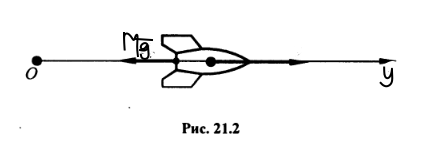
\includegraphics[scale=0.5]{img/21.2.jpeg} 
    \end{figure}

    \par\fbox{\begin{minipage}{20em}
        Ракету рисуйте вертикально! => ось Oy будет направлена вверх, а сила тяжести - вниз
    \end{minipage}}  
    
    \par 2) \quad $\frac{1}{2} a t^{2} => \alpha V_r = const$
    
    \par $y=-\frac{1}{2} g t^{2} + \frac{V_r}{\alpha}\left[(1-\alpha t)ln(1-\alpha t) + \alpha t \right]$

    \par $y=-\frac{1}{2} g t^{2} + \frac{1}{2}\alpha V_r t^{2} = \frac{1}{2}(\alpha V_r - g) t^{2}$
    
\end{center}
\end{document}